%!TEX TS-program = xelatex
%!TEX encoding = UTF-8

\documentclass[
	colors = false,
	geometry = a4,
	fontsetup = font-setup-overleaf.tex,
	titlesetup = titles-setup.tex
]{AJbook}

\usepackage{mathrsfs}
\usepackage{tikz}
\usetikzlibrary{arrows.meta,calc,patterns}
\usepackage{tikz-cd}
\usepackage{enumitem}
\usepackage{multicol}
\usepackage{environ}
\usepackage{myarrows}
\usepackage{mycommand}
\usepackage[unicode, bookmarksnumbered]{hyperref}

\AtEndPreamble{%
	\geometry{
		paperwidth=254mm,
		paperheight=359.21mm,
		left=1.2mm,
		right=1.2mm,
		top=1.2mm,
		bottom=1mm,
		headheight=0pt,
		headsep=0pt,
		footskip=0pt,
		includehead=false,
		includefoot=false
	}%
}

\pagestyle{empty}
\raggedbottom
\setstretch{0.8}
\setlength{\parindent}{0pt}
\setlength{\parskip}{0pt}
\setlength{\columnsep}{1.4mm}
\setlength{\multicolsep}{0pt}
\setlength{\premulticols}{0pt}
\setlength{\postmulticols}{0pt}
\setlength{\abovedisplayskip}{0pt plus 0.4pt}
\setlength{\belowdisplayskip}{0pt plus 0.4pt}
\setlength{\abovedisplayshortskip}{0pt plus 0.5pt}
\setlength{\belowdisplayshortskip}{0pt plus 0.5pt}
\setlength{\jot}{0pt}
\setlength{\emergencystretch}{8em}
\tolerance=9999
\hbadness=10000
\clubpenalty=0
\widowpenalty=0
\displaywidowpenalty=0
\interlinepenalty=0
\predisplaypenalty=0
\postdisplaypenalty=0
\brokenpenalty=0
\binoppenalty=0
\relpenalty=0
\mathsurround=0pt
\thinmuskip=1mu
\medmuskip=1.5mu plus 1mu minus 1mu
\thickmuskip=2mu plus 1mu minus 1mu
\allowdisplaybreaks[4]
\setlist{nosep,leftmargin=*,topsep=0pt,partopsep=0pt,parsep=0pt,itemsep=0pt}

\newcommand{\compactinlinetag}[1]{\quad\textup{(#1)}}
\AtBeginDocument{%
	\sloppy
	\renewcommand{\[}{\unskip\space\(\textstyle}%
	\renewcommand{\]}{\)\space\ignorespaces}%
	\RenewEnviron{equation}{\unskip\space\(\textstyle\BODY\)\space\ignorespaces}%
	\RenewEnviron{align*}{\unskip\space\(\textstyle\begin{aligned}\BODY\end{aligned}\)\space\ignorespaces}%
	\RenewEnviron{align}{\unskip\space\(\textstyle\begin{aligned}\BODY\end{aligned}\)\space\ignorespaces}%
	\let\tag\compactinlinetag
}

\hypersetup{
	pdfauthor = {王维桥},
	pdftitle = {数论基础笔记：压缩版},
	pdfkeywords = {Number Theory, Course Notes, 数论},
	CJKbookmarks = true
}

\addbibresource{references.bib}

\newenvironment{question}{%
	\par\noindent\textbf{问题.}\enspace
}{%
	\par
}
\newcommand{\todo}[1]{%
	\par\noindent\textcolor{black}{\textbf{TODO:} #1}\par
}
\newcommand{\weekmarker}[1]{}
\providecommand{\C}{\CC}
\providecommand{\U}[1]{(\Z/#1\Z)^\times}
\providecommand{\Cyc}[1]{\Z/#1\Z}
\providecommand{\e}[1]{e\!\left(#1\right)}
\providecommand{\expi}[1]{\exp(2\pi i #1)}
\providecommand{\cond}{\operatorname{cond}}

\makeatletter
\@beginparpenalty=0
\@endparpenalty=0
\@itempenalty=0
\@secpenalty=0
\renewcommand\chapter{%
	\par\addvspace{0.18\baselineskip}%
	\global\@topnum\z@
	\@afterindentfalse
	\secdef\compact@chapter\compact@schapter}
\def\compact@chapter[#1]#2{%
	\refstepcounter{chapter}%
	\addcontentsline{toc}{chapter}{\protect\numberline{\thechapter}#1}%
	\chaptermark{#1}%
	\noindent{\sffamily\bfseries\fontsize{6.4}{6.6}\selectfont \thechapter\enspace #2}\par\nobreak
	\vspace{0pt}%
	\@afterheading}
\def\compact@schapter#1{%
	\noindent{\sffamily\bfseries\fontsize{6.4}{6.6}\selectfont #1}\par\nobreak
	\vspace{0pt}%
	\@afterheading}
\makeatother

\titleformat{name=\section}[runin]
	{\sffamily\bfseries}
	{\thesection}
	{0.35em}
	{#1.}
\titleformat{name=\section, numberless}[runin]
	{\sffamily\bfseries}
	{}
	{0pt}
	{#1.}
\titlespacing*{name=\section}{0pt}{0.1\baselineskip}{0.45em}

\titleformat{name=\subsection}[runin]
	{\sffamily\bfseries}
	{\thesubsection}
	{0.3em}
	{#1.}
\titleformat{name=\subsection, numberless}[runin]
	{\sffamily\bfseries}
	{}
	{0pt}
	{#1.}
\titlespacing*{name=\subsection}{0pt}{0.06\baselineskip}{0.35em}

\titleformat{name=\subsubsection}[runin]
	{\sffamily\bfseries}
	{\thesubsubsection}
	{0.3em}
	{#1.}
\titleformat{name=\subsubsection, numberless}[runin]
	{\sffamily\bfseries}
	{}
	{0pt}
	{#1.}
\titlespacing*{name=\subsubsection}{0pt}{0.03\baselineskip}{0.3em}

\makeatletter
\renewcommand\section{\@ifstar\compactsectionstar\compactsection}
\newcommand\compactsection[1]{%
	\par\addvspace{0.04\baselineskip}%
	\refstepcounter{section}%
	\addcontentsline{toc}{section}{\protect\numberline{\thesection}#1}%
	\sectionmark{#1}%
	\noindent{\sffamily\bfseries\thesection\enspace #1.}\space\ignorespaces
}
\newcommand\compactsectionstar[1]{%
	\par\addvspace{0.04\baselineskip}%
	\sectionmark{#1}%
	\noindent{\sffamily\bfseries #1.}\space\ignorespaces
}
\renewcommand\subsection{\@ifstar\compactsubsectionstar\compactsubsection}
\newcommand\compactsubsection[1]{%
	\par\addvspace{0.02\baselineskip}%
	\refstepcounter{subsection}%
	\addcontentsline{toc}{subsection}{\protect\numberline{\thesubsection}#1}%
	\noindent{\sffamily\bfseries\thesubsection\enspace #1.}\space\ignorespaces
}
\newcommand\compactsubsectionstar[1]{%
	\par\addvspace{0.02\baselineskip}%
	\noindent{\sffamily\bfseries #1.}\space\ignorespaces
}
\renewcommand\subsubsection{\@ifstar\compactsubsubsectionstar\compactsubsubsection}
\newcommand\compactsubsubsection[1]{%
	\par\addvspace{0pt}%
	\refstepcounter{subsubsection}%
	\addcontentsline{toc}{subsubsection}{\protect\numberline{\thesubsubsection}#1}%
	\noindent{\sffamily\bfseries\thesubsubsection\enspace #1.}\space\ignorespaces
}
\newcommand\compactsubsubsectionstar[1]{%
	\par\addvspace{0pt}%
	\noindent{\sffamily\bfseries #1.}\space\ignorespaces
}
\makeatother

	\AtBeginDocument{%
		\pagestyle{empty}%
		\thispagestyle{empty}%
		\raggedright
		\fontsize{6.328}{6.518}\selectfont
		\setlength{\theorempreskipamount}{0pt}%
		\setlength{\theorempostskipamount}{0pt}%
		\theorempreskip{0pt}%
		\theorempostskip{0pt}%
		\theoremseparator{\ }%
		\theoremsymbol{}%
		\theorembodyfont{\fangsong}%
		\theoremheaderfont{\sffamily\bfseries\thmheiti}%
		\renewtheorem{theorem}{定理}[section]%
		\renewtheorem{corollary}[theorem]{推论}%
		\renewtheorem{lemma}[theorem]{引理}%
		\renewtheorem{proposition}[theorem]{命题}%
		\renewtheorem{definition}[theorem]{定义}%
		\renewtheorem{definition-theorem}[theorem]{定义--定理}%
		\renewtheorem{definition-proposition}[theorem]{定义--命题}%
		\renewtheorem{hypothesis}[theorem]{假设}%
		\renewtheorem{conjecture}[theorem]{猜想}%
		\theorembodyfont{\songti}%
		\renewtheorem{example}[theorem]{例}%
		\renewtheorem{remark}[theorem]{注记}%
		\renewtheorem{convention}[theorem]{约定}%
		\renewtheorem{exercise}[theorem]{练习}%
		\newcommand{\compactthmhead}[3]{%
			\par\noindent{\sffamily\bfseries #1#2%
			\if\relax\detokenize{#3}\relax\else\ (#3)\fi}%
			\enspace\ignorespaces
		}%
		\RenewDocumentEnvironment{theorem}{O{}}{%
			\refstepcounter{theorem}\compactthmhead{定理}{\thetheorem}{#1}\begingroup\fangsong
		}{\endgroup\par\ignorespacesafterend}%
		\RenewDocumentEnvironment{corollary}{O{}}{%
			\refstepcounter{theorem}\compactthmhead{推论}{\thetheorem}{#1}\begingroup\fangsong
		}{\endgroup\par\ignorespacesafterend}%
		\RenewDocumentEnvironment{lemma}{O{}}{%
			\refstepcounter{theorem}\compactthmhead{引理}{\thetheorem}{#1}\begingroup\fangsong
		}{\endgroup\par\ignorespacesafterend}%
		\RenewDocumentEnvironment{proposition}{O{}}{%
			\refstepcounter{theorem}\compactthmhead{命题}{\thetheorem}{#1}\begingroup\fangsong
		}{\endgroup\par\ignorespacesafterend}%
		\RenewDocumentEnvironment{definition}{O{}}{%
			\refstepcounter{theorem}\compactthmhead{定义}{\thetheorem}{#1}\begingroup\fangsong
		}{\endgroup\par\ignorespacesafterend}%
		\RenewDocumentEnvironment{definition-theorem}{O{}}{%
			\refstepcounter{theorem}\compactthmhead{定义--定理}{\thetheorem}{#1}\begingroup\fangsong
		}{\endgroup\par\ignorespacesafterend}%
		\RenewDocumentEnvironment{definition-proposition}{O{}}{%
			\refstepcounter{theorem}\compactthmhead{定义--命题}{\thetheorem}{#1}\begingroup\fangsong
		}{\endgroup\par\ignorespacesafterend}%
		\RenewDocumentEnvironment{hypothesis}{O{}}{%
			\refstepcounter{theorem}\compactthmhead{假设}{\thetheorem}{#1}\begingroup\fangsong
		}{\endgroup\par\ignorespacesafterend}%
		\RenewDocumentEnvironment{conjecture}{O{}}{%
			\refstepcounter{theorem}\compactthmhead{猜想}{\thetheorem}{#1}\begingroup\fangsong
		}{\endgroup\par\ignorespacesafterend}%
		\RenewDocumentEnvironment{example}{O{}}{%
			\refstepcounter{theorem}\compactthmhead{例}{\thetheorem}{#1}\begingroup\songti
		}{\endgroup\par\ignorespacesafterend}%
		\RenewDocumentEnvironment{remark}{O{}}{%
			\refstepcounter{theorem}\compactthmhead{注记}{\thetheorem}{#1}\begingroup\songti
		}{\endgroup\par\ignorespacesafterend}%
		\RenewDocumentEnvironment{convention}{O{}}{%
			\refstepcounter{theorem}\compactthmhead{约定}{\thetheorem}{#1}\begingroup\songti
		}{\endgroup\par\ignorespacesafterend}%
		\RenewDocumentEnvironment{exercise}{O{}}{%
			\refstepcounter{theorem}\compactthmhead{练习}{\thetheorem}{#1}\begingroup\songti
		}{\endgroup\par\ignorespacesafterend}%
		\renewenvironment{proof}[1][证明]{%
			\par\noindent{\sffamily\bfseries #1}\enspace\ignorespaces
		}{%
			\ifhmode\unskip\nobreak\hfill\openbox\par\else\leavevmode\hfill\openbox\par\fi
			\ignorespacesafterend
		}%
	}

\begin{document}

\begin{multicols}{2}
\setcounter{chapter}{-1}
% compact: skipped chapter 0 引子：素数与算术基本定理
\refstepcounter{chapter}% preserve original chapter numbering after skipping chapter 0
\chapter{算术函数}

\weekmarker{第 1 周}

% compact: skipped section 1.1 算术函数的例子
\refstepcounter{section}% preserve section numbering

\section{Dirichlet 卷积}

% compact: skipped definition 1.2.1
\refstepcounter{theorem}% preserve theorem numbering

\begin{remark}
	许多算术函数都可以通过卷积定义, 例如
	\(\textstyle \tau=\allowbreak{}u*u,\allowbreak{} \qquad \omega=\allowbreak{}u*\delta_{\mathbb P}.\)
	

\end{remark}

\begin{theorem}
	Dirichlet 卷积运算是交换，结合的
在逐点加法和 Dirichlet 卷积之下，$\mathcal A$ 中所有函数构成一个带单位元的交换环（unital commutative ring），乘法单位元为 $I(n)$。

\end{theorem}


\begin{theorem}[手稿标作 Thm 0]
	一个算术函数 $f$ 可逆，当且仅当
	\(
		f(1)\neq 0.
	\)
	如果 $f^{-1}$ 存在，则它是唯一的，并且由下式递归给出：
	\(\textstyle f^{-1}(1)=\allowbreak{}\frac{1}{f(1)},\allowbreak{}\)
	而当 $n>1$ 时，
	\(\textstyle f^{-1}(n) =\allowbreak{} -\frac{1}{f(1)} \sum_{d\mid\allowbreak{} n,\allowbreak{} d<n} f\left(\frac nd\right)f^{-1}(d).\)
\end{theorem}

\begin{proof}
	若 $f*g=I$，则代入 $n=1$ 得
	\(\textstyle f(1)g(1)=\allowbreak{}I(1)=\allowbreak{}1,\allowbreak{}\)
	从而 $f(1)\neq 0$。

	反过来，对满足 $f(1)\neq 0$ 的 $f\in\mathcal A$，我们用递归构造它的逆元 $f^{-1}$。先定义
	\(\textstyle f^{-1}(1)=\allowbreak{}\frac1{f(1)}.\)
	对 $n>1$，假设所有 $k<n$ 的 $f^{-1}(k)$ 已经定义。我们需要满足
	\(\textstyle f*f^{-1}(n)=\allowbreak{}I(n)=\allowbreak{}0.\)
	于是
	\(\textstyle 0 =\allowbreak{} \sum_{d\mid\allowbreak{} n} f(d)f^{-1}\left(\frac nd\right) =\allowbreak{} f(1)f^{-1}(n) +\allowbreak{} \sum_{d\mid\allowbreak{} n,\allowbreak{} d\neq\allowbreak{} 1} f(d)f^{-1}\left(\frac nd\right),\allowbreak{}\)
  从而得到上面的递归公式。由此可以定义出 $f^{-1}(n)$。唯一性由环的性质得到
\end{proof}

\section{Möbius 函数与 Möbius 反演}

回忆 Möbius 函数 $\mu$ 的定义。事实上也可以反过来定义
\(\textstyle \mu:=\allowbreak{}u^{-1},\allowbreak{}\)
也就是说，$\mu$ 是常值函数 $u(n)=1$ 的 Dirichlet 逆元，满足
\(\textstyle \mu*u=\allowbreak{}I.\)

\begin{proof}
只需证明:\(\textstyle \sum_{d\mid n}\mu(d)= \begin{cases} 1, & n=1,\\ 0, & n>1. \end{cases}\)
设 $n>1$的唯一分解为 $n=p_1^{\alpha_1} \cdots p_s^{\alpha_s}$, 
那么 \(\textstyle \sum_{d\mid\allowbreak{} n}\mu(d)=\allowbreak{}\sum_{d\mid\allowbreak{} p_1\cdots p_n}\mu(d)=\allowbreak{}\sum_{d\mid\allowbreak{} p_2\cdots p_n} \mu(p_1d)+\allowbreak{}\mu(d)=\allowbreak{}0\)

\end{proof}

\begin{exercise}
	证明
	\(\textstyle \sum_{d^2\mid\allowbreak{} n}\mu(d)=\allowbreak{}\mu^2(n).\)
\end{exercise}

% compact: skipped theorem 1.3.2 and its proof
\refstepcounter{theorem}% preserve theorem numbering

\begin{example}
	有
	\(\textstyle \varphi=\allowbreak{}\operatorname{id}*\mu,\allowbreak{}\)
	也即
	\(\textstyle \varphi(n) =\allowbreak{} \sum_{d\mid\allowbreak{} n}d\,\mu\left(\frac nd\right) =\allowbreak{} \sum_{d\mid\allowbreak{} n}\mu(d)\frac nd.\)
\end{example}

\begin{proof}
	等价地，只需证明
	\(\textstyle \varphi*u=\allowbreak{}\operatorname{id},\allowbreak{}\)
	即
	\(\textstyle \sum_{d\mid\allowbreak{} n}\varphi(d)=\allowbreak{}n.\)
	将集合 $\{1,2,\ldots,n\}$ 分解为互不相交的并：
	\(\textstyle \{1,\allowbreak{}2,\allowbreak{}\ldots,\allowbreak{}n\} =\allowbreak{} \coprod_{d\mid\allowbreak{} n} A(d),\allowbreak{} \qquad A(d):=\allowbreak{}\{k\leq\allowbreak{} n:(k,\allowbreak{}n)=\allowbreak{}d\}.\)
	对 $k\in A(d)$，令 $c=k/d$，则
	\(\textstyle 1\leq\allowbreak{} c\leq\allowbreak{} \frac nd,\allowbreak{}\qquad \left(c,\allowbreak{}\frac nd\right)=\allowbreak{}1.\)
	因此
	\(\textstyle |A(d)| =\allowbreak{} \#\left\{1\leq\allowbreak{} c\leq\allowbreak{} \frac nd:\left(c,\allowbreak{}\frac nd\right)=\allowbreak{}1\right\} =\allowbreak{} \varphi\left(\frac nd\right).\)
	于是
	\(\textstyle n =\allowbreak{} \sum_{d\mid\allowbreak{} n}\varphi\left(\frac nd\right) =\allowbreak{} \sum_{d\mid\allowbreak{} n}\varphi(d).\)
\end{proof}

\begin{example}
	有
	\(\textstyle \log=\allowbreak{}\Lambda*u,\allowbreak{}\)
	等价地
	\(\textstyle \Lambda=\allowbreak{}\log*\mu.\)
	也就是说
	\(\textstyle \log n=\allowbreak{}\sum_{d\mid\allowbreak{} n}\Lambda(d).\)
\end{example}

\begin{proof}
	$n=1$ 时显然成立。若 $n>1$，写
	\(\textstyle n=\allowbreak{}p_1^{\alpha_1}\cdots p_r^{\alpha_r}.\)
	左边为
	\(\textstyle \log n =\allowbreak{} \log\left(p_1^{\alpha_1}\cdots p_r^{\alpha_r}\right) =\allowbreak{} \sum_{i=\allowbreak{}1}^r \alpha_i\log p_i.\)
	右边为
	\(\textstyle \sum_{d\mid\allowbreak{} n}\Lambda(d) =\allowbreak{} \sum_{i=\allowbreak{}1}^r\sum_{m=\allowbreak{}1}^{\alpha_i}\Lambda(p_i^m) =\allowbreak{} \sum_{i=\allowbreak{}1}^r\alpha_i\log p_i =\allowbreak{} \log n.\)
\end{proof}

\section{乘法函数}

\begin{definition}[乘法函数（multiplicative function）]
	算术函数 $f\in\mathcal A$ 称为乘法函数，如果 $f$ 不恒等于零，并且只要 $(m,n)=1$，就有
	\(\textstyle f(mn)=\allowbreak{}f(m)f(n).\)
	如果对所有 $m,n$ 都有
	\(\textstyle f(mn)=\allowbreak{}f(m)f(n),\allowbreak{}\)
	则称 $f$ 为完全乘法函数（completely multiplicative function）。
\end{definition}

\begin{corollary}
	若 $f,g$ 是乘法函数，则 $fg$ 也是乘法函数；若 $g(n)\neq 0$，则 $f/g$ 也是乘法函数。完全乘法函数的情形同理。
\end{corollary}

\begin{example}
	$\mu(n)$、$\tau(n)$ 是乘法函数。
\end{example}

\begin{example}
	函数 $n^\alpha$（$\alpha\in\CC$）以及
	\(\textstyle I(n)= \begin{cases} 1, & n=1,\\ 0, & n>1 \end{cases}\)
	是完全乘法函数。
\end{example}

\begin{example}
	$\varphi(n)$ 是乘法函数。
\end{example}

\begin{proof}
	由 CRT。
\end{proof}

% compact: skipped theorem 1.4.6 and its proof
\refstepcounter{theorem}% preserve theorem numbering

% compact: skipped remark 1.4.7
\refstepcounter{theorem}% preserve theorem numbering

\begin{theorem}
	有如下两个结论：(a) 如果 $f$ 和 $g$ 都是乘法函数，则 $f*g$ 也是乘法函数；(b) 如果 $g$ 和 $f*g$ 都是乘法函数，则 $f$ 也是乘法函数。
\end{theorem}

\begin{proof}
	先证 (a)。设 $(n_1,n_2)=1$。则
	\(\textstyle (f*g)(n_1n_2) =\allowbreak{} \sum_{d\mid\allowbreak{} n_1n_2}f(d)g\left(\frac{n_1n_2}{d}\right).\)
	因为 $(n_1,n_2)=1$，每个 $d\mid n_1n_2$ 唯一写成 $d=d_1d_2$，其中 $d_1\mid n_1$、$d_2\mid n_2$。因此
	\(\textstyle (f*g)(n_1n_2) =\allowbreak{} \sum_{d_1\mid\allowbreak{} n_1,\allowbreak{} d_2\mid\allowbreak{} n_2} f(d_1d_2)g\left(\frac{n_1}{d_1}\frac{n_2}{d_2}\right)\) \(\textstyle =\allowbreak{} \left(\sum_{d_1\mid\allowbreak{} n_1}f(d_1)g\left(\frac{n_1}{d_1}\right)\right) \left(\sum_{d_2\mid\allowbreak{} n_2}f(d_2)g\left(\frac{n_2}{d_2}\right)\right)\) \(\textstyle =\allowbreak{}(f*g)(n_1)(f*g)(n_2).\)

	再证 (b)。反设 $f$ 不是乘法函数。只需证明 $h:=f*g$ 不是乘法函数。由于 $f$ 不是乘法函数，存在 $(m,n)=1$ 使得
	\(\textstyle f(mn)\neq\allowbreak{} f(m)f(n).\)
	若 $mn=1$，则 $f(1)\neq f(1)^2$，从而 $f(1)\neq 1$；由于 $g$ 是乘法函数，$g(1)=1$，所以
	\(\textstyle h(1)=\allowbreak{}f*g(1)=\allowbreak{}f(1)g(1)\neq\allowbreak{} 1,\allowbreak{}\)
	故 $h$ 不是乘法函数。

	若 $mn>1$，取乘积 $mn$ 在所有反例中最小。此时若 $d_1\mid m$、$d_2\mid n$ 且 $d_1d_2<mn$，则由最小性有
	\(\textstyle f(d_1d_2)=\allowbreak{}f(d_1)f(d_2).\)
	于是
	\(\textstyle h(mn) =\allowbreak{} \sum_{d\mid\allowbreak{} mn}f(d)g\left(\frac{mn}{d}\right)\) \(\textstyle =\allowbreak{} \sum_{d_1\mid\allowbreak{} m,\allowbreak{} d_2\mid\allowbreak{} n,\allowbreak{} d_1d_2<mn} f(d_1d_2) g\left(\frac{mn}{d_1d_2}\right) +\allowbreak{} f(mn)g(1)\) \(\textstyle =\allowbreak{} \sum_{d_1\mid\allowbreak{} m,\allowbreak{} d_2\mid\allowbreak{} n} f(d_1)g\left(\frac m{d_1}\right) f(d_2)g\left(\frac n{d_2}\right) - f(m)g(1)f(n)g(1) +\allowbreak{} f(mn)\) \(\textstyle =\allowbreak{} h(m)h(n)-f(m)f(n)+\allowbreak{}f(mn)\) \(\textstyle \neq\allowbreak{} h(m)h(n).\)
	所以 $h$ 不是乘法函数，矛盾推出 (b)。
\end{proof}

\begin{remark}
	即使 $f$ 和 $g$ 都是完全乘法函数，也不能推出 $f*g$ 完全乘法。例如
	\(\textstyle \tau=\allowbreak{}u*u.\)
\end{remark}

\begin{corollary}
	如果 $f$ 是乘法函数，则
	\(\textstyle F(n):=\allowbreak{}\sum_{d\mid\allowbreak{} n}f(d) =\allowbreak{} \prod_{p^\alpha\Vert n}\bigl(1+\allowbreak{}f(p)+\allowbreak{}\cdots+\allowbreak{}f(p^\alpha)\bigr).\)
\end{corollary}

\begin{proof}
	因为 $F=u*f$ 是乘法函数，所以若 $n=p_1^{\alpha_1}\cdots p_r^{\alpha_r}$，则
	\(\textstyle F(n) =\allowbreak{} F(p_1^{\alpha_1})\cdots F(p_r^{\alpha_r}) =\allowbreak{} \prod_{p^\alpha\Vert n}\bigl(1+\allowbreak{}f(p)+\allowbreak{}\cdots+\allowbreak{}f(p^\alpha)\bigr).\)
\end{proof}

\begin{corollary}
	如果 $f$ 是乘法函数，则
	\(\textstyle \sum_{d\mid\allowbreak{} n}\mu(d)f(d) =\allowbreak{} \prod_{p\mid\allowbreak{} n}\bigl(1-f(p)\bigr).\)
\end{corollary}

\begin{proof}
	在上一个推论中取算术函数 $d\mapsto \mu(d)f(d)$。它是乘法函数，于是
	\(\textstyle \sum_{d\mid\allowbreak{} n}\mu(d)f(d) =\allowbreak{} \prod_{p^\alpha\Vert n} \bigl(1+\allowbreak{}\mu(p)f(p)+\allowbreak{}\cdots+\allowbreak{}\mu(p^\alpha)f(p^\alpha)\bigr) =\allowbreak{} \prod_{p\mid\allowbreak{} n}(1-f(p)).\)
\end{proof}

% compact: skipped corollary 1.4.12 and its proof
\refstepcounter{theorem}% preserve theorem numbering

% compact: skipped theorem 1.4.13 and its proof
\refstepcounter{theorem}% preserve theorem numbering

\begin{theorem}
	设 $f$ 是乘法函数。则 $f$ 是完全乘法函数，当且仅当
	\(\textstyle f^{-1}(n)=\allowbreak{}\mu(n)f(n),\allowbreak{}\qquad \forall n\geq\allowbreak{} 1.\)
\end{theorem}

\begin{proof}
	先设 $f$ 是完全乘法函数。定义
	\(\textstyle g(n)=\allowbreak{}\mu(n)f(n).\)
	则
	\(\textstyle (f*g)(n) =\allowbreak{} \sum_{d\mid\allowbreak{} n}f\left(\frac nd\right)\mu(d)f(d) =\allowbreak{} f(n)\sum_{d\mid\allowbreak{} n}\mu(d) =\allowbreak{} I(n).\)
	所以 $g$ 是 $f$ 的 Dirichlet 逆元。

	反过来，假设
	\(\textstyle f^{-1}(n)=\allowbreak{}\mu(n)f(n).\)
	我们要证明 $f$ 是完全乘法函数。因为 $f$ 已经是乘法函数，只需证明对所有素数 $p$ 和 $\alpha\geq 1$ 都有
	\(\textstyle f(p^\alpha)=\allowbreak{}f(p)^\alpha.\)
	由
	\(\textstyle f*f^{-1}=\allowbreak{}I\)
	并取 $n=p^\alpha$，得到
	\(\textstyle \sum_{d\mid\allowbreak{} p^\alpha} f(d)\mu\left(\frac{p^\alpha}{d}\right)f\left(\frac{p^\alpha}{d}\right) =\allowbreak{}0.\)
	由于 $\mu(p^j)=0$ 当 $j\geq 2$，上式只剩
	\(\textstyle \mu(1)f(1)f(p^\alpha)+\allowbreak{}\mu(p)f(p)f(p^{\alpha-1})=\allowbreak{}0.\)
	因此
	\(\textstyle f(p^\alpha)=\allowbreak{}f(p)f(p^{\alpha-1}),\allowbreak{}\)
	递归可得
	\(\textstyle f(p^\alpha)=\allowbreak{}f(p)^\alpha.\)
\end{proof}

% compact: skipped exercise 1.4.15
\refstepcounter{theorem}% preserve theorem numbering

\begin{example}
	令 $\varphi$ 为 Euler 函数。断言
	\(\textstyle \varphi^{-1}=\allowbreak{}(\mu\cdot\operatorname{id})*u,\allowbreak{}\)
	其中 $\mu\cdot\operatorname{id}$ 表示逐点乘积。
\end{example}

\begin{proof}
	回忆
	\(\textstyle \varphi=\allowbreak{}\operatorname{id}*\mu.\)
	因为 $\operatorname{id}(n)=n$ 是完全乘法函数，所以
	\(\textstyle \operatorname{id}^{-1}=\allowbreak{}\mu\cdot\operatorname{id}.\)
	于是
	\(\textstyle \varphi^{-1} =\allowbreak{} (\operatorname{id}*\mu)^{-1} =\allowbreak{} \operatorname{id}^{-1}*\mu^{-1} =\allowbreak{} (\mu\cdot\operatorname{id})*u.\)
	也就是说
	\(\textstyle \varphi^{-1}(n)=\allowbreak{}\sum_{d\mid\allowbreak{} n}\mu(d)d.\)
\end{proof}

\section{Liouville 函数}

回忆 Liouville 函数
\(\textstyle \lambda(n)=\allowbreak{}(-1)^{\Omega(n)} =\allowbreak{} (-1)^{\alpha_1+\allowbreak{}\cdots+\allowbreak{}\alpha_r} \quad \text{若 } n=\allowbreak{}p_1^{\alpha_1}\cdots p_r^{\alpha_r}.\)

\begin{remark}
	$\lambda(n)$ 是完全乘法函数，因为
	\(\textstyle \Omega(nm)=\allowbreak{}\Omega(n)+\allowbreak{}\Omega(m),\allowbreak{}\qquad \forall n,\allowbreak{}m.\)
\end{remark}

\begin{theorem}
	对每个 $n\geq 1$，有
	\(\textstyle \sum_{d\mid n}\lambda(d) = \begin{cases} 1, & n\text{ 是平方数},\\ 0, & \text{otherwise}. \end{cases}\)
	此外，
	\(\textstyle \lambda^{-1}(n)=\allowbreak{}|\mu(n)|,\allowbreak{}\qquad \forall n.\)
\end{theorem}

\begin{proof}
	因为 $\lambda$ 是乘法函数，所以
	\(\textstyle (u*\lambda)(n)=\allowbreak{}\sum_{d\mid\allowbreak{} n}\lambda(d)\)
	也是乘法函数。因此只需检查等式两边在素数幂 $n=p^\alpha$ 上相等。

	对 $n=p^\alpha$，左边为
	\(\textstyle \sum_{d\mid\allowbreak{} p^\alpha}\lambda(d) =\allowbreak{} \lambda(1)+\allowbreak{}\lambda(p)+\allowbreak{}\cdots+\allowbreak{}\lambda(p^\alpha) =\allowbreak{} (-1)^0+\allowbreak{}(-1)^1+\allowbreak{}\cdots+\allowbreak{}(-1)^\alpha.\)
	故当 $\alpha$ 为奇数时该和为 $0$，当 $\alpha$ 为偶数时该和为 $1$，这正是右边。

	第二个结论来自上一个定理。因为 $\lambda$ 完全乘法，所以
	\(\textstyle \lambda^{-1}(n) =\allowbreak{} \mu(n)\lambda(n) =\allowbreak{} \mu(n)^2 =\allowbreak{} |\mu(n)|.\)
\end{proof}

\section{Selberg 恒等式}

回忆 von Mangoldt 函数
\(\textstyle \Lambda(n)= \begin{cases} \log p, & n=p^k\ (k\geq 1),\\ 0, & \text{otherwise}. \end{cases}\)
我们已经证明
\(\textstyle \log=\allowbreak{}\Lambda*u,\allowbreak{}\)
等价地
\(\textstyle \Lambda=\allowbreak{}\mu*\log.\)
展开卷积定义，得到
\(\textstyle \Lambda(n) =\allowbreak{} \sum_{d\mid\allowbreak{} n}\mu(d)\log\frac nd =\allowbreak{} \log n\sum_{d\mid\allowbreak{} n}\mu(d) -\sum_{d\mid\allowbreak{} n}\mu(d)\log d.\)
由于 $\log n\sum_{d\mid n}\mu(d)=\log n\,I(n)=0$，因此
\(\textstyle \Lambda=\allowbreak{}-(\mu\cdot\log)*u,\allowbreak{}\)
其中 $\mu\cdot\log$ 表示逐点乘积。

\begin{definition}[广义 von Mangoldt 函数（generalized von Mangoldt function）]
	对 $k\geq 0$，定义
	\(\textstyle \Lambda_k(n) =\allowbreak{} \sum_{d\mid\allowbreak{} n}\mu(d)\left(\log\frac nd\right)^k.\)
	也即
	\(\textstyle \Lambda_k=\allowbreak{}\mu*\log^k,\allowbreak{}\)
	其中 $\log^k(n):=(\log n)^k$。
\end{definition}

\begin{remark}
	有
	\(\textstyle \Lambda_0=\allowbreak{}I,\allowbreak{}\qquad \Lambda_1=\allowbreak{}\Lambda.\)
\end{remark}

\begin{theorem}[Selberg 恒等式（Selberg's identity）]
	有
	\(\textstyle \Lambda_k =\allowbreak{} \Lambda_{k-1}\log+\allowbreak{}\Lambda_{k-1}*\Lambda,\allowbreak{}\)
	其中 $\Lambda_{k-1}\log$ 表示逐点乘积。
\end{theorem}

\begin{proof}
	由 $\Lambda_{k-1}=\mu*\log^{k-1}$ 得 $\log^{k-1}=u*\Lambda_{k-1}$。同时展开 $\log(n/d)=\log n-\log d$，于是
	\(\textstyle \Lambda_k =\allowbreak{}\mu*\log^k\) \(\textstyle =\allowbreak{}(\mu*\log^{k-1})\log-(\mu\cdot\log)*\log^{k-1}\) \(\textstyle =\allowbreak{}\Lambda_{k-1}\log-(\mu\cdot\log)*(u*\Lambda_{k-1})\) \(\textstyle =\allowbreak{}\Lambda_{k-1}\log+\allowbreak{}\Lambda*\Lambda_{k-1}\) \(\textstyle =\allowbreak{}\Lambda_{k-1}\log+\allowbreak{}\Lambda_{k-1}*\Lambda.\)
\end{proof}

% compact: skipped remark 1.6.4
\refstepcounter{theorem}% preserve theorem numbering


% compact: skipped exercise 1.6.5
\refstepcounter{theorem}% preserve theorem numbering


\chapter{算术函数的平均值}

\weekmarker{第 2 周}

% compact: skipped section 2.1 若干记号
\refstepcounter{section}% preserve section numbering
\section{用积分近似}

\weekmarker{第 2 周}

算术函数最简单的例子之一来自连续函数。若 $f$ 不剧烈振荡，我们有理由相信
\(\textstyle \sum_{n\leq\allowbreak{} x}f(n)\sim\allowbreak{} \int_1^x f(\xi)\,d\xi.\)

\begin{theorem}
	设 $f:[y,x]\to\R$ 是单调函数。则
	\(\textstyle \sum_{y<n\leq\allowbreak{} x} f(n) =\allowbreak{} \int_y^x f(\xi)\,d\xi +\allowbreak{} O\bigl(|f(y)|+\allowbreak{}|f(x)|\bigr).\)
\end{theorem}

\begin{proof}
	我们可以假设 $f$ 递增。对任意 $y<n\leq x$，有
	\(\textstyle \int_{n-1}^{n} f(\xi)\,d\xi \leq\allowbreak{} f(n) \leq\allowbreak{} \int_{n}^{n+\allowbreak{}1} f(\xi)\,d\xi.\)
	对所有满足 $y+1\leq n\leq x$ 的整数 $n$ 求和，得到
	\(\textstyle \int_y^x f(\xi)\,d\xi \leq\allowbreak{} \sum_{y<n\leq\allowbreak{} x} f(n) \leq\allowbreak{} \int_y^x f(\xi)\,d\xi+\allowbreak{}O\bigl(|f(y)|+\allowbreak{}|f(x)|\bigr).\)
	递减情形同理。
\end{proof}

\begin{example}
	函数 $f(x)=\log x$ 是单调的。因此
	\(\textstyle \sum_{n\leq\allowbreak{} x}\log n =\allowbreak{} \int_1^x\log \xi\,d\xi+\allowbreak{}O(\log x).\)
	计算积分可得
	\(\textstyle \sum_{n\leq\allowbreak{} x}\log n =\allowbreak{} x\log x-x+\allowbreak{}O(\log x).\)
\end{example}

不过，并不是很多函数都是单调的。

\begin{theorem}[Euler--Maclaurin 公式]
	设 $f:[y,x]\to\CC$ 连续可微。定义
	\(\textstyle \psi(\xi):=\allowbreak{}\{\xi\}-\frac12,\allowbreak{}\)
	其中 $\{\xi\}$ 表示 $\xi$ 的小数部分。则
	\(\textstyle \sum_{y<n\leq\allowbreak{} x} f(n) =\allowbreak{} \int_y^x f(\xi)\,d\xi +\allowbreak{} \int_y^x \psi(\xi)f'(\xi)\,d\xi +\allowbreak{} \psi(y)f(y)-\psi(x)f(x).\)
\end{theorem}

\begin{proof}
	先考虑 $y,x$ 为整数的情形。我们有如下断言：对所有整数 $n$，
	\(\textstyle \frac{f(n+\allowbreak{}1)+\allowbreak{}f(n)}{2} =\allowbreak{} \int_n^{n+\allowbreak{}1} f(\xi)\,d\xi +\allowbreak{} \int_n^{n+\allowbreak{}1}\left(\xi-n-\frac12\right)f'(\xi)\,d\xi.\)
	这个断言由分部积分得到：
	\(\textstyle \int_n^{n+\allowbreak{}1}\left(\xi-n-\frac12\right)f'(\xi)\,d\xi =\allowbreak{} \left.\left(\xi-n-\frac12\right)f(\xi)\right|_n^{n+\allowbreak{}1} - \int_n^{n+\allowbreak{}1}f(\xi)\,d\xi,\allowbreak{}\)
	于是右边等于 $\frac{f(n+1)+f(n)}2$。

	对上式在区间上求和。具体说，对 $y\leq n\leq x-1$ 求和，得到
	\(\textstyle \sum_{y\leq\allowbreak{} n\leq\allowbreak{} x-1}\frac{f(n+\allowbreak{}1)+\allowbreak{}f(n)}2 =\allowbreak{} \int_y^x f(\xi)\,d\xi +\allowbreak{} \int_y^x\psi(\xi)f'(\xi)\,d\xi.\)
	左边为
	\(\textstyle \sum_{y<n\leq\allowbreak{} x}f(n)+\allowbreak{}\frac{f(y)}2-\frac{f(x)}2 =\allowbreak{} \sum_{y<n\leq\allowbreak{} x}f(n)+\allowbreak{}\psi(y)f(y)-\psi(x)f(x).\)
	这就完成了整数端点情形。

	现在处理一般的 $y,x\in\R$。这里 $[t]$ 表示 $t$ 的整数部分。由整数端点情形，
	\(\textstyle \sum_{y<n\leq\allowbreak{} x}f(n) =\allowbreak{} f([y]+\allowbreak{}1)+\allowbreak{}\sum_{[y]+\allowbreak{}1<n\leq\allowbreak{} [x]}f(n).\)
	因此
	\(\textstyle \sum_{y<n\leq\allowbreak{} x}f(n) =\allowbreak{}{}f([y]+\allowbreak{}1) +\allowbreak{}\int_{[y]+\allowbreak{}1}^{[x]}f(\xi)\,d\xi +\allowbreak{}\int_{[y]+\allowbreak{}1}^{[x]}\psi(\xi)f'(\xi)\,d\xi\) \(\textstyle +\allowbreak{}\psi([y]+\allowbreak{}1)f([y]+\allowbreak{}1)-\psi([x])f([x]).\)
	也即
	\(\textstyle \sum_{y<n\leq\allowbreak{} x}f(n) =\allowbreak{}{} \int_y^x f(\xi)\,d\xi +\allowbreak{}\int_y^x \psi(\xi)f'(\xi)\,d\xi\) \(\textstyle -\int_{[x]}^x f(\xi)\,d\xi -\int_y^{[y]+\allowbreak{}1}f(\xi)\,d\xi -\int_{[x]}^x\psi(\xi)f'(\xi)\,d\xi -\int_y^{[y]+\allowbreak{}1}\psi(\xi)f'(\xi)\,d\xi\) \(\textstyle +\allowbreak{}\frac{f([y]+\allowbreak{}1)+\allowbreak{}f([x])}{2}.\)
		% compact: skipped figure in theorem 2.2.3 proof
	观察到
	\(\textstyle \int_{[x]}^x f(\xi)\,d\xi +\allowbreak{} \int_{[x]}^x\psi(\xi)f'(\xi)\,d\xi =\allowbreak{} \psi(x)f(x)+\allowbreak{}\frac12 f([x]).\)
	类似地，
	\(\textstyle \int_y^{[y]+\allowbreak{}1} f(\xi)\,d\xi +\allowbreak{} \int_y^{[y]+\allowbreak{}1}\psi(\xi)f'(\xi)\,d\xi =\allowbreak{} -\psi(y)f(y)+\allowbreak{}\frac12 f([y]+\allowbreak{}1).\)
	最终得到
	\(\textstyle \sum_{y<n\leq\allowbreak{} x}f(n) =\allowbreak{} \int_y^x f(\xi)\,d\xi +\allowbreak{} \int_y^x \psi(\xi)f'(\xi)\,d\xi +\allowbreak{} \psi(y)f(y)-\psi(x)f(x).\)
\end{proof}

\begin{corollary}[原文 Corollary 1]
	有
	\(\textstyle \sum_{n\leq\allowbreak{} x}\frac1n =\allowbreak{} \log x+\allowbreak{}\gamma+\allowbreak{}O\left(\frac1x\right),\allowbreak{}\)
	其中
	\(\textstyle \gamma =\allowbreak{} 1-\int_1^\infty\frac{\{\xi\}}{\xi^2}\,d\xi\)
	是 Euler 常数（Euler constant）。
\end{corollary}

\begin{proof}
	由 Euler--Maclaurin 公式，
	\(\textstyle \sum_{n\leq\allowbreak{} x}\frac1n =\allowbreak{} 1+\allowbreak{}\sum_{1<n\leq\allowbreak{} x}\frac1n\) \(\textstyle =\allowbreak{} 1+\allowbreak{}\int_1^x\frac1\xi\,d\xi -\int_1^x\frac{\psi(\xi)}{\xi^2}\,d\xi +\allowbreak{}\psi(1)-\psi(x)\frac1x\) \(\textstyle =\allowbreak{} 1+\allowbreak{}\log x-\int_1^\infty\frac{\psi(\xi)}{\xi^2}\,d\xi +\allowbreak{}\int_x^\infty\frac{\psi(\xi)}{\xi^2}\,d\xi -\frac12+\allowbreak{}O\left(\frac1x\right)\) \(\textstyle =\allowbreak{} \frac12+\allowbreak{}\log x -\int_1^\infty\frac{\{\xi\}}{\xi^2}\,d\xi +\allowbreak{}\frac12\int_1^\infty\frac{d\xi}{\xi^2} +\allowbreak{}O\left(\frac1x\right)\) \(\textstyle =\allowbreak{} \log x+\allowbreak{}1-\int_1^\infty\frac{\{\xi\}}{\xi^2}\,d\xi +\allowbreak{}O\left(\frac1x\right)\) \(\textstyle =\allowbreak{} \log x+\allowbreak{}\gamma+\allowbreak{}O\left(\frac1x\right).\)
\end{proof}

% compact: skipped remark 2.2.5
\refstepcounter{theorem}% preserve theorem numbering


\section{卷积方法}

\weekmarker{第 2 周}

若
\(\textstyle h=\allowbreak{}f*g,\allowbreak{}\)
并且如果我们可以估计 $g$ 的部分和，那么
\(\textstyle \sum_{n\leq\allowbreak{} x}h(n) =\allowbreak{} \sum_{n\leq\allowbreak{} x}\sum_{dm=\allowbreak{}n}f(d)g(m)\) \(\textstyle =\allowbreak{} \sum_{d\leq\allowbreak{} x}f(d)\sum_{m\leq\allowbreak{} x/d}g(m).\)

\begin{theorem}[原文 Theorem 3]
	有
	\(\textstyle \sum_{n\leq\allowbreak{} x}\varphi(n) =\allowbreak{} Cx^2+\allowbreak{}O(x\log x),\allowbreak{} \qquad C=\allowbreak{}\frac{3}{\pi^2}.\)
\end{theorem}

\begin{proof}
	回忆
	\(\textstyle \varphi=\allowbreak{}\operatorname{id}*\mu,\allowbreak{} \qquad \varphi(n)=\allowbreak{}\sum_{d\mid\allowbreak{} n}\mu(d)\frac nd.\)
	于是
	\(\textstyle \sum_{n\leq\allowbreak{} x}\varphi(n) =\allowbreak{} \sum_{d\leq\allowbreak{} x}\mu(d)\sum_{m\leq\allowbreak{} x/d}m\) \(\textstyle =\allowbreak{} \sum_{d\leq\allowbreak{} x}\mu(d) \left(\frac12\left(\frac xd\right)^2+\allowbreak{}O\left(\frac xd\right)\right)\) \(\textstyle =\allowbreak{} \frac{x^2}{2}\sum_{d\leq\allowbreak{} x}\frac{\mu(d)}{d^2} +\allowbreak{} O\left(x\sum_{d\leq\allowbreak{} x}\frac1d\right)\) \(\textstyle =\allowbreak{} \frac{x^2}{2} \left(\sum_{d=\allowbreak{}1}^\infty\frac{\mu(d)}{d^2} -\sum_{d>x}\frac{\mu(d)}{d^2}\right) +\allowbreak{}O(x\log x)\) \(\textstyle =\allowbreak{} \frac{x^2}{2}\sum_{d=\allowbreak{}1}^\infty\frac{\mu(d)}{d^2} +\allowbreak{}O\left(x^2\sum_{d>x}\frac1{d^2}+\allowbreak{}x\log x\right)\) \(\textstyle =\allowbreak{} \frac{x^2}{2\zeta(2)}+\allowbreak{}O(x\log x).\)
	由于 $\zeta(2)=\pi^2/6$，所以 $C=3/\pi^2$。
\end{proof}

% compact: skipped remark 2.3.2
\refstepcounter{theorem}% preserve theorem numbering


% compact: skipped theorem 2.3.3 and its proof
\refstepcounter{theorem}% preserve theorem numbering


% compact: skipped remark 2.3.4
\refstepcounter{theorem}% preserve theorem numbering


\begin{proposition}[原文 Proposition 1]
	对任意正整数 $A$，存在无穷多个 $n\in\N$，使得
	\(\textstyle (\log n)^A<\tau(n).\)
\end{proposition}

\begin{proof}
	取固定互异的素数 $p_1,p_2,\ldots,p_{A+1}$，并考虑
	\(\textstyle n=\allowbreak{}(p_1p_2\cdots p_{A+\allowbreak{}1})^r,\allowbreak{}\)
	其中 $r\geq 1$ 是任意整数。则
	\(\textstyle \tau(n) =\allowbreak{} \tau(p_1^r)\cdots \tau(p_{A+\allowbreak{}1}^r) =\allowbreak{} (r+\allowbreak{}1)^{A+\allowbreak{}1}.\)
	另一方面，
	\(\textstyle (\log n)^A =\allowbreak{} r^A(\log p_1+\allowbreak{}\cdots+\allowbreak{}\log p_{A+\allowbreak{}1})^A.\)
	由于 $r$ 可以任意大，所以存在无穷多个这样的 $n$ 使
	\(\textstyle (\log n)^A\leq\allowbreak{} \tau(n).\)
\end{proof}

\begin{proposition}[原文 Proposition 2]
	对任意给定的 $\varepsilon>0$，存在 $C_\varepsilon>0$，使得对所有 $n\in\N$，
	\(\textstyle \tau(n)\leq\allowbreak{} C_\varepsilon n^\varepsilon.\)
	换句话说，
	\(\textstyle \tau(n)\ll\allowbreak{} n^\varepsilon \qquad\text{或}\qquad \tau(n)=\allowbreak{}O(n^\varepsilon).\)
\end{proposition}

% compact: skipped proof of proposition 2.3.6


误差项 $O(x)$ 对
\(\textstyle \sum_{n\leq\allowbreak{} x}\tau(n)\)
而言并不令人满意。为了改进它，我们引入 Dirichlet 双曲线方法（Dirichlet hyperbola method）。

% compact: skipped section title Dirichlet 双曲线方法
\refstepcounter{section}% preserve section numbering

\weekmarker{第 2 周}

\begin{theorem}
	设
	\(\textstyle h=\allowbreak{}f*g.\)
	那么对任意 $y\leq x$，有
	\(\textstyle \sum_{n\leq\allowbreak{} x}h(n) =\allowbreak{}{} \sum_{d\leq\allowbreak{} y}f(d)\sum_{m\leq\allowbreak{} x/d}g(m) +\allowbreak{} \sum_{m\leq\allowbreak{} x/y}g(m)\sum_{d\leq\allowbreak{} x/m}f(d)\) \(\textstyle - \left(\sum_{d\leq\allowbreak{} y}f(d)\right) \left(\sum_{m\leq\allowbreak{} x/y}g(m)\right).\)
\end{theorem}

\begin{proof}
	我们要计算
	\(\textstyle \sum_{n\leq\allowbreak{} x}h(n) =\allowbreak{} \sum_{dm\leq\allowbreak{} x}f(d)g(m).\)
	% compact: skipped Dirichlet hyperbola figure in theorem 2.4.1 proof
	于是
	\(\textstyle \sum_{n\leq\allowbreak{} x}h(n) =\allowbreak{}{} \sum_{d\leq\allowbreak{} y}f(d)\sum_{m\leq\allowbreak{} x/d}g(m) +\allowbreak{} \sum_{m\leq\allowbreak{} x/y}g(m)\sum_{d\leq\allowbreak{} x/m}f(d)\) \(\textstyle - \sum_{d\leq\allowbreak{} y}f(d)\sum_{m\leq\allowbreak{} x/y}g(m).\)
\end{proof}

\begin{theorem}[原文 Theorem 4]
	有
	\(\textstyle \sum_{n\leq\allowbreak{} x}\tau(n) =\allowbreak{} x\log x+\allowbreak{}(2\gamma-1)x+\allowbreak{}O(x^{1/2}).\)
\end{theorem}

\begin{proof}
	取 $y=\sqrt{x}$。由于
	\(\textstyle \tau=\allowbreak{}u*u,\allowbreak{}\)
	由 Dirichlet 双曲线方法得到
	\(\textstyle \sum_{n\leq\allowbreak{} x}\tau(n) =\allowbreak{} 2\sum_{d\leq\allowbreak{} \sqrt{x}}\left[\frac xd\right]-[\sqrt{x}]^2\) \(\textstyle =\allowbreak{} 2\sum_{d\leq\allowbreak{} \sqrt{x}}\left(\frac xd+\allowbreak{}O(1)\right) -\bigl(\sqrt{x}+\allowbreak{}O(1)\bigr)^2\) \(\textstyle =\allowbreak{} 2x\sum_{d\leq\allowbreak{} \sqrt{x}}\frac1d +\allowbreak{}O\left(\sum_{d\leq\allowbreak{} \sqrt{x}}1\right) -x+\allowbreak{}O(x^{1/2})\) \(\textstyle =\allowbreak{} 2x\left(\log\sqrt{x}+\allowbreak{}\gamma+\allowbreak{}O(x^{-1/2})\right) -x+\allowbreak{}O(x^{1/2})\) \(\textstyle =\allowbreak{} x\log x+\allowbreak{}(2\gamma-1)x+\allowbreak{}O(x^{1/2}).\)
\end{proof}

% compact: skipped remark 2.4.3
\refstepcounter{theorem}% preserve theorem numbering

只有有限的一类算术函数 $h\in A$ 可以写成 Dirichlet 卷积
\(\textstyle h=\allowbreak{}f*g.\)
问题是：如果我们知道 $f(n)$ 的部分和
\(\textstyle \sum_{m\leq\allowbreak{} y}f(m),\allowbreak{}\)
那么如何估计乘积
\(\textstyle h(n)=\allowbreak{}f(n)g(n),\allowbreak{}\)
其中 $g$ 是一个比较好的函数？这由 Abel 求和提供。

\section{Abel 求和公式}

\weekmarker{第 2 周}

\begin{theorem}[Abel 求和公式；原文 Theorem 5]
	设 $f$ 是一个算术函数，且 $g:[y,x]\to\CC$ 连续可微。则
	\(\textstyle \sum_{y<n\leq\allowbreak{} x}f(n)g(n) =\allowbreak{}{} \left(\sum_{n\leq\allowbreak{} x}f(n)\right)g(x) - \left(\sum_{n\leq\allowbreak{} y}f(n)\right)g(y)\) \(\textstyle - \int_y^x \left(\sum_{n\leq\allowbreak{} \xi}f(n)\right)g'(\xi)\,d\xi.\)
\end{theorem}

\begin{proof}
	另一种写法是
	\(\textstyle \sum_{y<n\leq\allowbreak{} x}f(n)g(n) =\allowbreak{} \int_y^x g(\xi)\,d\sum_{y<n\leq\allowbreak{} \xi}f(n).\)
	下面证明手稿中的离散版本。我们可以假设
	\(\textstyle [y]+\allowbreak{}1\leq\allowbreak{} [x].\)
	记
	\(\textstyle F(x):=\allowbreak{}\sum_{n\leq\allowbreak{} x}f(n).\)
	则
	\(\textstyle \text{LHS} =\allowbreak{} \sum_{y<n\leq\allowbreak{} x}\bigl(F(n)-F(n-1)\bigr)g(n)\) \(\textstyle =\allowbreak{} \sum_{y<n\leq\allowbreak{} x}F(n)g(n) - \sum_{y+\allowbreak{}1<n\leq\allowbreak{} x}F(n-1)g(n)\) \(\textstyle =\allowbreak{} \sum_{y<n\leq\allowbreak{} x-1}F(n)\bigl(g(n)-g(n+\allowbreak{}1)\bigr) +\allowbreak{} F([x])g([x])-F([y])g([y]+\allowbreak{}1)\) \(\textstyle =\allowbreak{} -\sum_{y<n\leq\allowbreak{} x-1}F(n)\int_n^{n+\allowbreak{}1}g'(\xi)\,d\xi +\allowbreak{} F([x])g([x])-F([y])g([y]+\allowbreak{}1)\) \(\textstyle =\allowbreak{} -\int_{[y]+\allowbreak{}1}^{[x]}F(\xi)g'(\xi)\,d\xi +\allowbreak{} F([x])g([x])-F([y])g([y]+\allowbreak{}1).\)
	最后注意到
	\(\textstyle F(x)g([x]) =\allowbreak{} F(x)g(x)-\int_{[x]}^xF(\xi)g'(\xi)\,d\xi,\allowbreak{}\)
	以及
	\(\textstyle F(y)g([y]+\allowbreak{}1) =\allowbreak{} F(y)g(y)+\allowbreak{}\int_y^{[y]+\allowbreak{}1}F(\xi)g'(\xi)\,d\xi.\)
	于是得到
	\(\textstyle \text{LHS} =\allowbreak{} -\int_y^x F(\xi)g'(\xi)\,d\xi+\allowbreak{}F(x)g(x)-F(y)g(y),\allowbreak{}\)
	这正是右边。
\end{proof}

\begin{example}
	回忆在 Theorem 3 中已经证明
	\(\textstyle \sum_{n\leq\allowbreak{} x}\varphi(n)=\allowbreak{}Cx^2+\allowbreak{}O(x\log x),\allowbreak{} \qquad C=\allowbreak{}\frac3{\pi^2}.\)
	利用它可以证明下面的结论。
\end{example}

\begin{theorem}[原文 Theorem 6]
	有
	\(\textstyle \sum_{n\leq\allowbreak{} x}\frac{\varphi(n)}n =\allowbreak{} 2Cx+\allowbreak{}O(\log^2 x).\)
\end{theorem}

\begin{proof}
	由 Abel 求和，取 $g(\xi)=1/\xi$，得到
	\(\textstyle \sum_{n\leq\allowbreak{} x}\varphi(n)\frac1n =\allowbreak{} 1+\allowbreak{} \left(\sum_{n\leq\allowbreak{} x}\varphi(n)\right)\frac1x - \left(\sum_{n\leq\allowbreak{} 1}\varphi(n)\right)\cdot 1 -\int_1^x \left(\sum_{n\leq\allowbreak{} \xi}\varphi(n)\right) \left(\frac1\xi\right)'\,d\xi\) \(\textstyle =\allowbreak{} \frac1x\bigl(Cx^2+\allowbreak{}O(x\log x)\bigr) +\allowbreak{} \int_1^x \bigl(C\xi^2+\allowbreak{}O(\xi\log \xi)\bigr)\frac1{\xi^2}\,d\xi\) \(\textstyle =\allowbreak{} Cx+\allowbreak{}O(\log x) +\allowbreak{} C\int_1^x d\xi +\allowbreak{} O\left(\int_1^x\frac{\log \xi}{\xi}\,d\xi\right)\) \(\textstyle =\allowbreak{} 2Cx+\allowbreak{}O(\log x)+\allowbreak{}O(\log^2 x)\) \(\textstyle =\allowbreak{} 2Cx+\allowbreak{}O(\log^2 x).\)
\end{proof}

至于单个的 $\varphi(n)$，有下面的尖锐下界。

\begin{theorem}[原文 Theorem 7]
	有
	\(\textstyle \varphi(n)\gg\allowbreak{} \frac{n}{\log\log n}.\)
\end{theorem}

\begin{proof}
	回忆
	\(\textstyle \varphi(p^\alpha)=\allowbreak{}p^\alpha\left(1-\frac1p\right).\)
	于是
	\(\textstyle \frac{\varphi(n)}n =\allowbreak{} \prod_{p\mid\allowbreak{} n}\left(1-\frac1p\right).\)

	于是
	\(\textstyle \log\frac{\varphi(n)}n =\allowbreak{} \sum_{p\mid\allowbreak{} n}\log\left(1-\frac1p\right)\) \(\textstyle =\allowbreak{} -\sum_{p\mid\allowbreak{} n}\frac1p +\allowbreak{} \sum_{p\mid\allowbreak{} n} \left(\log\left(1-\frac1p\right)+\allowbreak{}\frac1p\right). \quad\textup{(*1)}\)
	回忆 Taylor 展开
	\(\textstyle \log(1-x)=\allowbreak{}-x-\frac{x^2}{2}-\cdots.\)
	因此
	\(\textstyle \sum_{p\mid\allowbreak{} n} \left(\log\left(1-\frac1p\right)+\allowbreak{}\frac1p\right) \ll\allowbreak{} \sum_{p\mid\allowbreak{} n}\frac1{p^2} \ll\allowbreak{} \sum_{m=\allowbreak{}1}^\infty\frac1{m^2} \ll\allowbreak{} 1.\)
	对于第一项，我们写
	\(\textstyle \sum_{p\mid\allowbreak{} n}\frac1p =\allowbreak{} \sum_{p\mid\allowbreak{} n,\allowbreak{} p<\log n}\frac1p +\allowbreak{} \sum_{p\mid\allowbreak{} n,\allowbreak{} p\geq\allowbreak{} \log n}\frac1p. \quad\textup{(*2)}\)
	若记 $p_1,p_2,\ldots,p_{r-\ell}$ 为整除 $n$ 且小于 $\log n$ 的不同素数，并记
	\(\textstyle p_{r-\ell+\allowbreak{}1},\allowbreak{}\ldots,\allowbreak{}p_r\)
	为整除 $n$ 且大于 $\log n$ 的素数，其中有 $\ell$ 个，则
	\(\textstyle (\log n)^\ell \leq\allowbreak{} \prod_{k=\allowbreak{}r-\ell+\allowbreak{}1}^r p_k \leq\allowbreak{} n.\)
	从而
	\(\textstyle \ell\leq\allowbreak{} \frac{\log n}{\log\log n}.\)
	把这个用于 $(*2)$ 的第二项，可得
	\(\textstyle \sum_{p\mid\allowbreak{} n,\allowbreak{} p>\log n}\frac1p \leq\allowbreak{} \frac1{\log n}\cdot \frac{\log n}{\log\log n} =\allowbreak{} O(1).\)
	现在考虑第一项。如果我们使用 Mertens 定理（Mertens' theorem）之一：
	\(\textstyle \sum_{p\leq\allowbreak{} x}\frac1p =\allowbreak{} \log\log x+\allowbreak{}C+\allowbreak{}O\left(\frac1{\log x}\right),\allowbreak{}\)
	原文旁注：to be proved later，则回到 $(*2)$ 有
	\(\textstyle \sum_{p\mid\allowbreak{} n}\frac1p \leq\allowbreak{} \log\log\log n+\allowbreak{}O(1).\)
	代入 $(*1)$，得到
	\(\textstyle \log\frac{\varphi(n)}n \geq\allowbreak{} -\log\log\log n+\allowbreak{}O(1),\allowbreak{}\)
	因此
	\(\textstyle \frac{\varphi(n)}n\gg\allowbreak{} \frac1{\log\log n},\allowbreak{}\)
	也就是
	\(\textstyle \varphi(n)\gg\allowbreak{} \frac{n}{\log\log n}.\)
\end{proof}

\begin{remark}
	\begin{enumerate}[label=(\alph*)]
		\item 如果避免使用 Mertens 定理，那么我们会有
		\(\textstyle \sum_{p\mid\allowbreak{} n,\allowbreak{} p<\log n}\frac1p \leq\allowbreak{} \sum_{m\leq\allowbreak{} \log n}\frac1m \ll\allowbreak{} \log\log n.\)
		这只会推出
		\(\textstyle \frac{\varphi(n)}n\gg\allowbreak{} \frac1{\log n}.\)
		\item 作为练习，可以证明存在一个递增序列 $n_k$，使得
		\(\textstyle \varphi(n_k)\ll\allowbreak{} \frac{n_k}{\log\log n_k}.\)
		因此 Theorem 7 中的下界是 sharp。
	\end{enumerate}
\end{remark}

\chapter{素数分布的初等结果}

\section{素数定理的等价形式}

\weekmarker{第 3 周}

回忆素数定理（Prime Number Theorem）断言：当 $x\to\infty$ 时，
\(\textstyle \pi(x):=\allowbreak{}\sum_{p\leq\allowbreak{} x}1\sim\allowbreak{} \frac{x}{\log x},\allowbreak{}\)
或者等价地，
\(\textstyle \lim_{x\to\allowbreak{}\infty}\frac{\pi(x)}{x/\log x}=\allowbreak{}1.\)
Legendre 和 Gauss 曾独立猜想该结论。有时用权重来数素数更有用。为此我们引入两个函数：
\(\textstyle \theta(x)=\allowbreak{}\sum_{p\leq\allowbreak{} x}\log p\)
以及
\(\textstyle \psi(x)=\allowbreak{}\sum_{n\leq\allowbreak{} x}\Lambda(n),\allowbreak{}\)
其中
\(\textstyle \Lambda(n)= \begin{cases} \log p, & n=p^k,\ k\geq 1,\\ 0, & \text{otherwise}, \end{cases}\)
是 von Mangoldt 函数（von Mangoldt function）。$\psi(x)$ 通常称为 Chebyshev 函数（Chebyshev function）。

回忆
\(\textstyle \log n=\allowbreak{}\sum_{d\mid\allowbreak{} n}\Lambda(d),\allowbreak{}\)
也即
\(\textstyle \log=\allowbreak{}\Lambda*u.\)
由 Möbius 反演（Möbius inversion），这等价于
\(\textstyle \Lambda=\allowbreak{}\log*\mu.\)

\begin{lemma}[原文 Lemma 3.1]
	有
	\(\textstyle \psi(x)=\allowbreak{}\theta(x)+\allowbreak{}O(x^{1/2}\log x).\)
\end{lemma}

\begin{proof}
	由定义，
	\(\textstyle \psi(x) =\allowbreak{} \sum_{n\leq\allowbreak{} x}\Lambda(n) =\allowbreak{} \sum_{p^m\leq\allowbreak{} x}\log p\) \(\textstyle =\allowbreak{} \sum_{p\leq\allowbreak{} x}\log p +\allowbreak{} \sum_{p^m\leq\allowbreak{} x,\allowbreak{} m\geq\allowbreak{} 2}\log p\) \(\textstyle =\allowbreak{} \theta(x)+\allowbreak{} \sum_{p\leq\allowbreak{} x^{1/2}}\log p \sum_{2\leq\allowbreak{} m\leq\allowbreak{} \log x/\log p}1\) \(\textstyle =\allowbreak{} \theta(x)+\allowbreak{} O\left( \sum_{p\leq\allowbreak{} x^{1/2}}\log p\cdot \frac{\log x}{\log p} \right)\) \(\textstyle =\allowbreak{} \theta(x)+\allowbreak{}O(x^{1/2}\log x).\)
\end{proof}

\begin{theorem}[原文 Theorem 3.2]
	以下三个命题等价：(i) $\pi(x)\sim \frac{x}{\log x}$；(ii) $\theta(x)\sim x$；(iii) $\psi(x)\sim x$。
\end{theorem}

\begin{proof}
	由 Lemma 3.1，只需要证明 $(i)\Longleftrightarrow(ii)$。

	先证明 $(i)\Rightarrow(ii)$。假设
	\(\textstyle \pi(x)\sim\allowbreak{} \frac{x}{\log x}.\)
	由 Abel 求和，
	\(\textstyle \theta(x) =\allowbreak{} \sum_{p\leq\allowbreak{} x}\log p\) \(\textstyle =\allowbreak{} \sum_{1<n\leq\allowbreak{} x}\mathbf 1_{n\in\mathbb P}\log n\) \(\textstyle =\allowbreak{} \left(\sum_{p\leq\allowbreak{} x}1\right)\log x - \int_1^x \frac{\sum_{p\leq\allowbreak{} y}1}{y}\,dy\) \(\textstyle =\allowbreak{} \pi(x)\log x-\int_1^x\frac{\pi(y)}y\,dy\) \(\textstyle =\allowbreak{} x+\allowbreak{}o(x)+\allowbreak{} O\left(\int_1^x\frac{dy}{\log y}\right).\)
	由于
	\(\textstyle \int_1^x\frac{dy}{\log y} =\allowbreak{} \int_1^{\sqrt{x}}\frac{dy}{\log y} +\allowbreak{} \int_{\sqrt{x}}^x\frac{dy}{\log y} \ll\allowbreak{} \sqrt{x}+\allowbreak{}\frac{x}{\log x} \ll\allowbreak{} \frac{x}{\log x},\allowbreak{}\)
	所以
	\(\textstyle \theta(x)=\allowbreak{}x+\allowbreak{}o(x).\)

	反过来，假设
	\(\textstyle \theta(x)\sim\allowbreak{} x.\)
	再次由 Abel 求和，
	\(\textstyle \pi(x) =\allowbreak{} \sum_{3/2<n\leq\allowbreak{} x}\log n\,\mathbf 1_{n\in\mathbb P}\cdot \frac1{\log n}\) \(\textstyle =\allowbreak{} \left(\sum_{p\leq\allowbreak{} x}\log p\right)\frac1{\log x} +\allowbreak{} \int_{3/2}^{x} \frac{\sum_{p\leq\allowbreak{} y}\log p}{y\log^2 y}\,dy\) \(\textstyle =\allowbreak{} \frac{x+\allowbreak{}o(x)}{\log x} +\allowbreak{} \int_{3/2}^{x}\frac{y+\allowbreak{}o(y)}{y\log^2 y}\,dy\) \(\textstyle =\allowbreak{} \frac{x}{\log x}+\allowbreak{}o\left(\frac{x}{\log x}\right) +\allowbreak{} O\left(\int_{3/2}^{x}\frac{dy}{\log^2 y}\right).\)
	利用类似的估计，
	\(\textstyle \int_{3/2}^{x}\frac{dy}{\log^2 y} \ll\allowbreak{} \frac{x}{\log^2 x} =\allowbreak{} o\left(\frac{x}{\log x}\right).\)
	因此
	\(\textstyle \pi(x)\sim\allowbreak{} \frac{x}{\log x}.\)
\end{proof}

Chebyshev 对素数定理作出了第一个重要贡献。

\section{Chebyshev 定理}

\begin{theorem}[原文 Theorem 3.3]
	有
	\(\textstyle \pi(x)\asymp\allowbreak{} \frac{x}{\log x},\allowbreak{} \qquad \theta(x)\asymp\allowbreak{} x,\allowbreak{} \qquad \psi(x)\asymp\allowbreak{} x.\)
\end{theorem}

\begin{proof}
	我们先建立
	\(\textstyle \psi(x)\ll\allowbreak{} x.\)
	记
	\(\textstyle S(x):=\allowbreak{}\sum_{n\leq\allowbreak{} x}\log n-2\sum_{n\leq\allowbreak{} x/2}\log n.\)
	回忆
	\(\textstyle \sum_{n\leq\allowbreak{} y}\log n=\allowbreak{}y\log y-y+\allowbreak{}O(\log y).\)
	因此
	\(\textstyle S(x) =\allowbreak{} x\log x-x -2\left(\frac x2\log\frac x2-\frac x2\right) +\allowbreak{}O(\log x)\) \(\textstyle =\allowbreak{} (\log 2)x+\allowbreak{}O(\log x). \quad\textup{(*1)}\)
	又回忆
	\(\textstyle \log=\allowbreak{}\Lambda*u.\)
	那么
	\(\textstyle \sum_{n\leq\allowbreak{} y}\log n =\allowbreak{} \sum_{d\leq\allowbreak{} y}\Lambda(d)\left[\frac yd\right].\)
	于是
	\(\textstyle S(x) =\allowbreak{} \sum_{d\leq\allowbreak{} x}\Lambda(d)\left[\frac xd\right] - 2\sum_{d\leq\allowbreak{} x/2}\Lambda(d)\left[\frac{x}{2d}\right]\) \(\textstyle =\allowbreak{} \sum_{d\leq\allowbreak{} x}\Lambda(d) \left(\left[\frac xd\right]-2\left[\frac{x}{2d}\right]\right). \quad\textup{(*2)}\)
	注意到对所有 $\alpha\geq 1$，
	\(\textstyle [\alpha]-2\left[\frac\alpha2\right]\in\{0,\allowbreak{}1\},\allowbreak{}\)
	并且当 $1\leq \alpha<2$ 时，
	\(\textstyle [\alpha]-2\left[\frac\alpha2\right]=\allowbreak{}1.\)
	由 $(*2)$ 得
	\(\textstyle \psi(x)-\psi\left(\frac x2\right) =\allowbreak{} \sum_{x/2<d\leq\allowbreak{} x}\Lambda(d) \leq\allowbreak{} S(x) \leq\allowbreak{} \sum_{d\leq\allowbreak{} x}\Lambda(d)=\allowbreak{}\psi(x).\)
	从 $(*1)$ 可见
	\(\textstyle S(x)\sim\allowbreak{} (\log 2)x,\allowbreak{}\)
	所以
	\(\textstyle \psi(x)\geq\allowbreak{} S(x)\gg\allowbreak{} x.\)
	另一方面，对每个 $x/2^j$，有
	\(\textstyle \psi\left(\frac{x}{2^j}\right) - \psi\left(\frac{x}{2^{j+\allowbreak{}1}}\right) \leq\allowbreak{} S\left(\frac{x}{2^j}\right) \ll\allowbreak{} \frac{x}{2^j}.\)
	对所有 $j\geq 0$ 求和，得到
	\(\textstyle \psi(x) =\allowbreak{} \sum_{j=\allowbreak{}0}^\infty \left( \psi\left(\frac{x}{2^j}\right) - \psi\left(\frac{x}{2^{j+\allowbreak{}1}}\right) \right) \ll\allowbreak{} x\sum_{j=\allowbreak{}0}^\infty\frac1{2^j} \ll\allowbreak{} x.\)
	因此
	\(\textstyle \psi(x)\asymp\allowbreak{} x,\allowbreak{}\)
	并且由 Lemma 3.1 也有
	\(\textstyle \theta(x)\asymp\allowbreak{} x.\)

	最后证明
	\(\textstyle \pi(x)\asymp\allowbreak{} \frac{x}{\log x}.\)
	注意
	\(\textstyle \pi(x)=\allowbreak{}\sum_{p\leq\allowbreak{} x}1 \geq\allowbreak{} \frac1{\log x}\sum_{p\leq\allowbreak{} x}\log p \gg\allowbreak{} \frac{x}{\log x}.\)
	另一方面，
	\(\textstyle \pi(x) \leq\allowbreak{} \sum_{p\leq\allowbreak{} \sqrt{x}}1 +\allowbreak{} \sum_{\sqrt{x}<p\leq\allowbreak{} x}\frac{\log p}{\log\sqrt{x}} \leq\allowbreak{} \sqrt{x}+\allowbreak{}\frac1{\log\sqrt{x}}\theta(x) \ll\allowbreak{} \frac{x}{\log x}.\)
	定理得证。
\end{proof}

\begin{corollary}[原文 Corollary 3.4]
	令 $p_r$ 为第 $r$ 个素数。则
	\(\textstyle p_r\asymp\allowbreak{} r\log r.\)
\end{corollary}

\begin{proof}
	在上面的定理中取 $x=p_r$，则
	\(\textstyle r=\allowbreak{}\pi(p_r)\asymp\allowbreak{} \frac{p_r}{\log p_r}.\)
	这推出
	\(\textstyle p_r\asymp\allowbreak{} r\log p_r\gg\allowbreak{} r\log r.\)
	另一方面，当 $p_r$ 足够大时，
	\(\textstyle \log p_r<p_r^{1/2}.\)
	于是
	\(\textstyle p_r\ll\allowbreak{} r\log p_r\ll\allowbreak{} r p_r^{1/2},\allowbreak{}\)
	从而
	\(\textstyle p_r\ll\allowbreak{} r^2.\)
	因此
	\(\textstyle p_r\asymp\allowbreak{} r\log p_r\ll\allowbreak{} r\log r.\)
\end{proof}

\section{Mertens 定理}

\begin{lemma}[原文 Lemma 3.5]
	有
	\(\textstyle \sum_{d\leq\allowbreak{} x}\frac{\Lambda(d)}d =\allowbreak{} \log x+\allowbreak{}O(1).\)
\end{lemma}

\begin{proof}
	从
	\(\textstyle \log=\allowbreak{}\Lambda*u\)
	出发，有
	\(\textstyle \sum_{n\leq\allowbreak{} x}\log n =\allowbreak{} \sum_{n\leq\allowbreak{} x}\sum_{d\mid\allowbreak{} n}\Lambda(d) =\allowbreak{} \sum_{d\leq\allowbreak{} x}\Lambda(d)\left[\frac xd\right]\) \(\textstyle =\allowbreak{} x\sum_{d\leq\allowbreak{} x}\frac{\Lambda(d)}d+\allowbreak{}O(x),\allowbreak{}\)
	其中用到了 $\psi(x)\ll x$。另一方面，
	\(\textstyle \sum_{n\leq\allowbreak{} x}\log n=\allowbreak{}x\log x-x+\allowbreak{}O(\log x).\)
	两边除以 $x$，得到
	\(\textstyle \sum_{d\leq\allowbreak{} x}\frac{\Lambda(d)}d=\allowbreak{}\log x+\allowbreak{}O(1).\)
\end{proof}

\begin{theorem}[原文 Theorem 3.6]
	有
	\(\textstyle \sum_{p\leq\allowbreak{} x}\frac{\log p}{p} =\allowbreak{} \log x+\allowbreak{}O(1).\)
\end{theorem}

\begin{proof}
	比较二者的差：
	\(\textstyle \left| \sum_{d\leq\allowbreak{} x}\frac{\Lambda(d)}d - \sum_{p\leq\allowbreak{} x}\frac{\log p}{p} \right| \leq\allowbreak{} \sum_{p^k\leq\allowbreak{} x,\allowbreak{} k\geq\allowbreak{} 2}\frac{\log p}{p^k}\) \(\textstyle \leq\allowbreak{} \sum_{p\leq\allowbreak{} \sqrt{x}}\log p \sum_{k=\allowbreak{}2}^{\log x/\log p}\frac1{p^k}\) \(\textstyle \leq\allowbreak{} \sum_{p\leq\allowbreak{} \sqrt{x}} \log p\cdot \frac{1/p^2}{1-1/p}\) \(\textstyle \leq\allowbreak{} \sum_p\frac{\log p}{p(p-1)} \ll\allowbreak{} 1.\)
	于是由 Lemma 3.5 得到结论。
\end{proof}

\begin{theorem}[原文 Theorem 3.7]
	存在常数 $C$，使得
	\(\textstyle \sum_{p\leq\allowbreak{} x}\frac1p =\allowbreak{} \log\log x+\allowbreak{}C+\allowbreak{}O\left(\frac1{\log x}\right).\)
\end{theorem}

\begin{proof}
	记
	\(\textstyle E(x):=\allowbreak{}\sum_{p\leq\allowbreak{} x}\frac{\log p}{p}-\log x.\)
	由 Theorem 3.6 可知
	\(\textstyle E(x)\ll\allowbreak{} 1.\)
	使用 Abel 求和，
	\(\textstyle \sum_{p\leq\allowbreak{} x}\frac1p =\allowbreak{} \sum_{3/2<n\leq\allowbreak{} x} \delta_{\mathbb P}(n)\frac{\log n}{n}\cdot\frac1{\log n}\) \(\textstyle =\allowbreak{} \left(\sum_{n\leq\allowbreak{} x}\delta_{\mathbb P}(n)\frac{\log n}{n}\right)\frac1{\log x} +\allowbreak{} \int_{3/2}^x \frac{\sum_{n\leq\allowbreak{} y}\delta_{\mathbb P}(n)\frac{\log n}{n}}{y\log^2 y}\,dy\) \(\textstyle =\allowbreak{} \frac{\log x+\allowbreak{}O(1)}{\log x} +\allowbreak{} \int_{3/2}^x\frac{\log y+\allowbreak{}E(y)}{y\log^2 y}\,dy\) \(\textstyle =\allowbreak{} \int_{3/2}^x\frac{dy}{y\log y} +\allowbreak{} \int_{3/2}^x\frac{E(y)}{y\log^2 y}\,dy +\allowbreak{} 1+\allowbreak{}O\left(\frac1{\log x}\right)\) \(\textstyle =\allowbreak{} \log\log x-\log\log\frac32 +\allowbreak{} \int_{3/2}^{\infty}\frac{E(y)}{y\log^2 y}\,dy - \int_x^\infty\frac{E(y)}{y\log^2 y}\,dy +\allowbreak{} 1+\allowbreak{}O\left(\frac1{\log x}\right).\)
	其中
	\(\textstyle \int_x^\infty\frac{E(y)}{y\log^2 y}\,dy \ll\allowbreak{} \int_x^\infty\frac{dy}{y\log^2 y} \ll\allowbreak{} \frac1{\log x},\allowbreak{}\)
	并且
	\(\textstyle \int_{3/2}^{\infty}\frac{E(y)}{y\log^2 y}\,dy\)
	是某个常数。于是
	\(\textstyle \sum_{p\leq\allowbreak{} x}\frac1p =\allowbreak{} \log\log x+\allowbreak{}C+\allowbreak{}O\left(\frac1{\log x}\right).\)
\end{proof}

\begin{theorem}[原文 Theorem 3.8]
	存在某个常数 $A$，使得
	\(\textstyle \prod_{p\leq\allowbreak{} x}\left(1-\frac1p\right) =\allowbreak{} \frac{A}{\log x} \left(1+\allowbreak{}O\left(\frac1{\log x}\right)\right).\)
\end{theorem}

\begin{proof}
	我们先考虑
	\(\textstyle \sum_{p\leq\allowbreak{} x}\log\left(1-\frac1p\right).\)
	使用 Taylor 展开，
	\(\textstyle \sum_{p\leq\allowbreak{} x}\log\left(1-\frac1p\right) =\allowbreak{} -\sum_{p\leq\allowbreak{} x}\frac1p +\allowbreak{} \sum_{p\leq\allowbreak{} x} \left(\log\left(1-\frac1p\right)+\allowbreak{}\frac1p\right)\) \(\textstyle =\allowbreak{} -\log\log x-C+\allowbreak{}O\left(\frac1{\log x}\right) +\allowbreak{} \sum_p \left(\log\left(1-\frac1p\right)+\allowbreak{}\frac1p\right)\) \(\textstyle \qquad - \sum_{p>x} \left(\log\left(1-\frac1p\right)+\allowbreak{}\frac1p\right).\)
	其中
	\(\textstyle \sum_p \left(\log\left(1-\frac1p\right)+\allowbreak{}\frac1p\right)=\allowbreak{}B\)
	是某个常数，因为
	\(\textstyle \sum_p \left(\log\left(1-\frac1p\right)+\allowbreak{}\frac1p\right) =\allowbreak{} -\sum_p\sum_{\ell\geq\allowbreak{} 2}\frac1{\ell p^\ell} \ll\allowbreak{} \sum_p\frac1{p^2} \ll\allowbreak{} \sum_{n\geq\allowbreak{} 1}\frac1{n^2} \ll\allowbreak{} 1.\)
	并且
	\(\textstyle \sum_{p>x} \left(\log\left(1-\frac1p\right)+\allowbreak{}\frac1p\right) \ll\allowbreak{} \sum_{p>x}\frac1{p^2} \ll\allowbreak{} \sum_{n>x}\frac1{n^2} \ll\allowbreak{} \frac1x.\)
	因此
	\(\textstyle \sum_{p\leq\allowbreak{} x}\log\left(1-\frac1p\right) =\allowbreak{} -\log\log x+\allowbreak{}A' +\allowbreak{} O\left(\frac1{\log x}\right).\)
	注意由 Taylor 展开，
	\(\textstyle \exp\left(O\left(\frac1{\log x}\right)\right) =\allowbreak{} 1+\allowbreak{}O\left(\frac1{\log x}\right).\)
	所以
	\(\textstyle \prod_{p\leq\allowbreak{} x}\left(1-\frac1p\right) =\allowbreak{} \exp\left(\sum_{p\leq\allowbreak{} x}\log\left(1-\frac1p\right)\right)\) \(\textstyle =\allowbreak{} \exp\left( -\log\log x+\allowbreak{}A' +\allowbreak{} O\left(\frac1{\log x}\right) \right)\) \(\textstyle =\allowbreak{} \frac{A}{\log x} \left(1+\allowbreak{}O\left(\frac1{\log x}\right)\right).\)
\end{proof}

接下来会介绍 Mertens 定理的一些应用。

\weekmarker{第 3 周}

\section{\texorpdfstring{\(\omega(n)\) 与 \(\Omega(n)\) 的平均值}{omega(n) 与 Omega(n) 的平均值}}

回忆，$\omega(n)$ 表示 $n$ 的不同素因子的个数，而 $\Omega(n)$ 表示 $n$ 的素因子的总个数，也就是说按重数计算。

对于单个的 $n$，$\omega(n)$ 与 $\Omega(n)$ 的行为可能相当不规则。但是在平均意义下，我们有下面的结果。

\begin{theorem}[原文 Theorem 3.9]
	有
	\(\textstyle \sum_{n\leq\allowbreak{} x}\omega(n) =\allowbreak{} x\log\log x+\allowbreak{}Cx+\allowbreak{}O\left(\frac{x}{\log x}\right),\allowbreak{}\)
	并且
	\(\textstyle \sum_{n\leq\allowbreak{} x}\Omega(n) =\allowbreak{} x\log\log x+\allowbreak{}C'x+\allowbreak{}O\left(\frac{x}{\log x}\right).\)
\end{theorem}

\begin{proof}
	先考虑 $\omega(n)$。有
	\(\textstyle \sum_{n\leq\allowbreak{} x}\omega(n) =\allowbreak{} \sum_{n\leq\allowbreak{} x}\sum_{p\mid\allowbreak{} n}1 =\allowbreak{} \sum_{p\leq\allowbreak{} x}\sum_{n\leq\allowbreak{} x,\allowbreak{} p\mid\allowbreak{} n}1\) \(\textstyle =\allowbreak{} \sum_{p\leq\allowbreak{} x}\left[\frac xp\right] =\allowbreak{} x\sum_{p\leq\allowbreak{} x}\frac1p+\allowbreak{}O\left(\sum_{p\leq\allowbreak{} x}1\right)\) \(\textstyle =\allowbreak{} x\left(\log\log x+\allowbreak{}C+\allowbreak{}O\left(\frac1{\log x}\right)\right) +\allowbreak{}O\left(\frac{x}{\log x}\right)\) \(\textstyle =\allowbreak{} x\log\log x+\allowbreak{}Cx+\allowbreak{}O\left(\frac{x}{\log x}\right),\allowbreak{}\)
	其中使用了 Mertens 定理以及 Chebyshev 定理给出的 $\pi(x)\ll x/\log x$。

	再考虑 $\Omega(n)$。有
	\(\textstyle \sum_{n\leq\allowbreak{} x}\Omega(n) =\allowbreak{} \sum_{n\leq\allowbreak{} x}\sum_{p^k\mid\allowbreak{} n}1 =\allowbreak{} \sum_{p^k\leq\allowbreak{} x}\sum_{n\leq\allowbreak{} x,\allowbreak{} p^k\mid\allowbreak{} n}1\) \(\textstyle =\allowbreak{} \sum_{p^k\leq\allowbreak{} x}\left[\frac{x}{p^k}\right]\) \(\textstyle =\allowbreak{} \sum_{p\leq\allowbreak{} x}\left[\frac xp\right] +\allowbreak{} \sum_{p^k\leq\allowbreak{} x,\allowbreak{} k\geq\allowbreak{} 2} \left[\frac{x}{p^k}\right]\) \(\textstyle =\allowbreak{} x\log\log x+\allowbreak{}Cx+\allowbreak{}O\left(\frac{x}{\log x}\right) +\allowbreak{} x\sum_{p^k\leq\allowbreak{} x,\allowbreak{} k\geq\allowbreak{} 2}\frac1{p^k} +\allowbreak{} O\left(\sum_{p^k\leq\allowbreak{} x,\allowbreak{} k\geq\allowbreak{} 2}1\right).\)
	原文在边栏证明下面这个估计：
	\(\textstyle \sum_{p^k>x,\allowbreak{} k\geq\allowbreak{} 2}\frac1{p^k} =\allowbreak{} O\left(x^{-1/2}\right).\)
	证明如下。若 $p\leq x^{1/2}$，则 $\log x/\log p\geq 2$，所以
	\(\textstyle \sum_{k\geq\allowbreak{} 2,\allowbreak{} p^k>x}\frac1{p^k} \leq\allowbreak{} \frac{1}{p^{\log x/\log p}}\cdot\frac1{1-1/p} \ll\allowbreak{} \frac1x\cdot\frac1{1-1/p}.\)
	若 $p>x^{1/2}$，则从 $k=2$ 起估计即可。因此
	\(\textstyle \sum_{p^k>x,\allowbreak{} k\geq\allowbreak{} 2}\frac1{p^k} \ll\allowbreak{} \frac1x\sum_{p\leq\allowbreak{} x^{1/2}}\frac1{1-1/p} +\allowbreak{} \sum_{p>x^{1/2}}\frac1{p^2}\frac1{1-1/p}\) \(\textstyle \ll\allowbreak{} \frac1x\sum_{p\leq\allowbreak{} x^{1/2}}1 +\allowbreak{} \sum_{n>x^{1/2}}\frac1{n^2} \ll\allowbreak{} x^{-1/2}.\)
	于是
	\(\textstyle \sum_{p^k\leq\allowbreak{} x,\allowbreak{} k\geq\allowbreak{} 2}\frac1{p^k} =\allowbreak{} \sum_{p,\allowbreak{} k\geq\allowbreak{} 2}\frac1{p^k} +\allowbreak{} O\left(x^{-1/2}\right) =\allowbreak{} C_1+\allowbreak{}O\left(x^{-1/2}\right).\)
	此外
	\(\textstyle \sum_{p^k\leq\allowbreak{} x,\allowbreak{} k\geq\allowbreak{} 2}1 \ll\allowbreak{} \sum_{p\leq\allowbreak{} x^{1/2}}\frac{\log x}{\log p} \ll\allowbreak{} x^{1/2}\log x.\)
	因此
	\(\textstyle \sum_{n\leq\allowbreak{} x}\Omega(n) =\allowbreak{} x\log\log x+\allowbreak{}Cx+\allowbreak{}O\left(\frac{x}{\log x}\right) +\allowbreak{} C_1x+\allowbreak{}O\left(x^{1/2}\right) +\allowbreak{} O\left(x^{1/2}\log x\right)\) \(\textstyle =\allowbreak{} x\log\log x+\allowbreak{}C'x+\allowbreak{}O\left(\frac{x}{\log x}\right).\)
\end{proof}

\begin{theorem}[原文 Theorem 3.10]
	有
	\(\textstyle \sum_{n\leq\allowbreak{} x}\omega^2(n) =\allowbreak{} x(\log\log x)^2+\allowbreak{}O(x\log\log x).\)
\end{theorem}

\begin{proof}
	考虑 $n$ 的不同素因子组成的有序对 $(p,q)$ 的个数，其中约定 $(p,q)$ 与 $(q,p)$ 作为两个不同的有序对来计算。于是有 $\omega(n)$ 种选择 $p$，当 $p$ 固定后有 $\omega(n)-1$ 种选择 $q$。因此
	\(\textstyle \omega(n)(\omega(n)-1) =\allowbreak{} \sum_{p\mid\allowbreak{} n,\allowbreak{} q\mid\allowbreak{} n,\allowbreak{} p\neq\allowbreak{} q}1.\)
	对 $n\leq x$ 求和，得到
	\(\textstyle \sum_{n\leq\allowbreak{} x}\omega(n)(\omega(n)-1) =\allowbreak{} \sum_{n\leq\allowbreak{} x} \sum_{p\mid\allowbreak{} n,\allowbreak{} q\mid\allowbreak{} n,\allowbreak{} p\neq\allowbreak{} q}1\) \(\textstyle =\allowbreak{} \sum_{pq\leq\allowbreak{} x,\allowbreak{} p\neq\allowbreak{} q} \sum_{n\leq\allowbreak{} x,\allowbreak{} pq\mid\allowbreak{} n}1 =\allowbreak{} \sum_{pq\leq\allowbreak{} x,\allowbreak{} p\neq\allowbreak{} q} \left[\frac{x}{pq}\right]\) \(\textstyle =\allowbreak{} x\sum_{pq\leq\allowbreak{} x,\allowbreak{} p\neq\allowbreak{} q}\frac1{pq} +\allowbreak{} O\left( \sum_{p\leq\allowbreak{} x}\sum_{q\leq\allowbreak{} x/p}1 \right).\)
	其中
	\(\textstyle \sum_{p\leq\allowbreak{} x}\sum_{q\leq\allowbreak{} x/p}1 \ll\allowbreak{} x\sum_{p\leq\allowbreak{} x}\frac1p \ll\allowbreak{} x\log\log x,\allowbreak{}\)
	这里再次使用 Mertens 定理。

	注意
	\(\textstyle \left(\sum_{p\leq\allowbreak{} x^{1/2}}\frac1p\right)^2 - \sum_{p\leq\allowbreak{} x^{1/2}}\frac1{p^2} \leq\allowbreak{} \sum_{pq\leq\allowbreak{} x,\allowbreak{} p\neq\allowbreak{} q}\frac1{pq} \leq\allowbreak{} \left(\sum_{p\leq\allowbreak{} x}\frac1p\right)^2.\)
	并且
	\(\textstyle \left(\sum_{p\leq\allowbreak{} x}\frac1p\right)^2 =\allowbreak{} (\log\log x+\allowbreak{}O(1))^2 =\allowbreak{} (\log\log x)^2+\allowbreak{}O(\log\log x),\allowbreak{}\)
	以及
	\(\textstyle \left(\sum_{p\leq\allowbreak{} x^{1/2}}\frac1p\right)^2 =\allowbreak{} (\log\log x^{1/2}+\allowbreak{}O(1))^2 =\allowbreak{} (\log\log x)^2+\allowbreak{}O(\log\log x).\)
	因此
	\(\textstyle \sum_{pq\leq\allowbreak{} x,\allowbreak{} p\neq\allowbreak{} q}\frac1{pq} =\allowbreak{} (\log\log x)^2+\allowbreak{}O(\log\log x).\)
	于是
	\(\textstyle \sum_{n\leq\allowbreak{} x}\omega(n)(\omega(n)-1) =\allowbreak{} x(\log\log x)^2+\allowbreak{}O(x\log\log x).\)
	最后，
	\(\textstyle \sum_{n\leq\allowbreak{} x}\omega^2(n) =\allowbreak{} \sum_{n\leq\allowbreak{} x}\omega(n)(\omega(n)-1) +\allowbreak{} \sum_{n\leq\allowbreak{} x}\omega(n)\) \(\textstyle =\allowbreak{} x(\log\log x)^2+\allowbreak{}O(x\log\log x).\)
\end{proof}

由 Theorem 3.9 和 Theorem 3.10，我们有充分理由相信，对大多数 $n$，$\omega(n)$ 的行为像
\(\textstyle \omega(n)\sim\allowbreak{} \log\log n.\)
这一点可以进一步说明如下。

\weekmarker{第 4 周}

\begin{theorem}[原文 Theorem 3.11]
	给定任意 $\varepsilon>0$。满足
	\(\textstyle \left|\omega(n)-\log\log n\right| > (\log\log n)^{1/2+\allowbreak{}\varepsilon}\)
	的 $n\in[1,x]$ 的个数至多是 $o(x)$。
\end{theorem}

\begin{proof}
	我们回忆 Chebyshev 不等式（Chebyshev inequality）的一个版本。设 $(X,\Sigma,\mu)$ 是一个测度空间（measure space），且 $f$ 可测。对 $0<p<\infty$，有
	\(\textstyle \mu\left(\left\{x\in X:|f(x)|>t\right\}\right) \leq\allowbreak{} \frac1{t^p}\int_{\{|f|>t\}}|f|^p\,d\mu.\)
	取 $p=2$，则
	\(\textstyle \#\left\{n\in[1,\allowbreak{}x]: \left|\omega(n)-\log\log x\right| > (\log\log x)^{1/2+\allowbreak{}\varepsilon} \right\}\) \(\textstyle \qquad\leq\allowbreak{} \frac1{(\log\log x)^{1+\allowbreak{}2\varepsilon}} \sum_{n\leq\allowbreak{} x}\left(\omega(n)-\log\log x\right)^2.\)
% compact: skipped remark 3.4.4
\refstepcounter{theorem}% preserve theorem numbering

	将区间分成
	\(\textstyle [1,\allowbreak{}x]=\allowbreak{}[1,\allowbreak{}x^{1/e}]\cup (x^{1/e},\allowbreak{}x].\)
	其中 $[1,x^{1/e}]$ 中的整数个数是 $o(x)$。对于 $n\in(x^{1/e},x]$，有
	\(\textstyle \log\log x-1=\allowbreak{}\log\log x^{1/e}<\log\log n\leq\allowbreak{} \log\log x.\)
	因此只需证明满足
	\(\textstyle \left|\omega(n)-\log\log x\right| > (\log\log x)^{1/2+\allowbreak{}\varepsilon}\)
	的 $n\in[1,x]$ 的个数 $M$ 是 $o(x)$。

	展开平方：
	\(\textstyle \sum_{n\leq\allowbreak{} x}\left(\omega(n)-\log\log x\right)^2 =\allowbreak{} \sum_{n\leq\allowbreak{} x}\omega^2(n) - 2\log\log x\sum_{n\leq\allowbreak{} x}\omega(n)\) \(\textstyle \qquad+\allowbreak{} [x](\log\log x)^2.\)
	由 Theorem 3.9 和 Theorem 3.10，
	\(\textstyle \sum_{n\leq\allowbreak{} x}\left(\omega(n)-\log\log x\right)^2 =\allowbreak{} x(\log\log x)^2+\allowbreak{}O(x\log\log x)\) \(\textstyle \quad -2\log\log x\left(x\log\log x+\allowbreak{}O(x)\right)\) \(\textstyle \quad +\allowbreak{}x(\log\log x)^2+\allowbreak{}O\left((\log\log x)^2\right)\) \(\textstyle =\allowbreak{} O(x\log\log x).\)
	因此
	\(\textstyle M \ll\allowbreak{} \frac{x\log\log x}{(\log\log x)^{1+\allowbreak{}2\varepsilon}} \ll\allowbreak{} \frac{x}{(\log\log x)^{2\varepsilon}} =\allowbreak{} o(x).\)
\end{proof}

\begin{remark}
	另一种做法是直接展开上面标记的平方项，并用 Abel 求和来估计
	\(\textstyle \sum_{n\leq\allowbreak{} x}\log\log n\cdot \omega(n),\allowbreak{}\)
	从而得到同样的结果。
\end{remark}

\begin{remark}
	\begin{enumerate}[label=(\alph*)]
		\item 同样的结论对 $\Omega(n)$ 也成立。
		\item Theorem 3.11 说明，对几乎所有 $n\in[1,x]$，都有
		\(\textstyle \omega(n),\allowbreak{}\ \Omega(n)\sim\allowbreak{} \log\log n.\)
		\item Erdős--Kac 定理（Erdős--Kac theorem, 1940）说明变量
		\(\textstyle \frac{\omega(n)-\log\log n}{\sqrt{\log\log n}}\)
		服从正态分布（normal distribution）。这是概率数论（Probabilistic Number Theory）的一个基本定理。
	\end{enumerate}
\end{remark}

\section{Bertrand 公设}

Bertrand 在 1845 年猜想：对每个 $n\geq 2$，总存在一个素数 $p$，使得
\(\textstyle n<p\leq\allowbreak{} 2n.\)
这个猜想由 Chebyshev 在 1852 年证明。

\begin{theorem}[Bertrand 公设；原文 Theorem 3.12]
	对任意 $n\geq 2$，至少存在一个素数
	\(\textstyle p\in(n,\allowbreak{}2n].\)
\end{theorem}

\begin{remark}
	可以从 Mertens 定理推出一个弱一些的版本。由
	\(\textstyle \sum_{p\leq\allowbreak{} x}\frac{\log p}{p}=\allowbreak{}\log x+\allowbreak{}O(1)\)
	可知，存在某个 $A>0$，使得
	\(\textstyle \log n-A < \sum_{p\leq\allowbreak{} n}\frac{\log p}{p} \leq\allowbreak{} \log n+\allowbreak{}A.\)
	于是
	\(\textstyle \sum_{n<p\leq\allowbreak{} e^{2A}n}\frac{\log p}{p} =\allowbreak{} \sum_{p\leq\allowbreak{} e^{2A}n}\frac{\log p}{p} - \sum_{p\leq\allowbreak{} n}\frac{\log p}{p}\) \(\textstyle > \log(e^{2A}n)-A-\log n-A =\allowbreak{} 0.\)
	因此存在素数 $p\in(n,e^{2A}n]$。
\end{remark}

为了证明 Theorem 3.12，我们先回忆下面的事实。

\begin{lemma}[原文 Lemma 3.13]
	令 $n\in\N$。记
	\(\textstyle n!:=\allowbreak{}\prod_{p\leq\allowbreak{} n}p^{h(p,\allowbreak{}n)}.\)
	则
	\(\textstyle h(p,\allowbreak{}n)=\allowbreak{}\sum_{r=\allowbreak{}1}^{\infty}\left[\frac{n}{p^r}\right].\)
\end{lemma}

% compact: skipped proof of lemma 3.5.3

\begin{lemma}[原文 Lemma 3.14]
	对每个正整数 $n$，有
	\(\textstyle \prod_{p\leq\allowbreak{} n}p<4^n.\)
\end{lemma}

\begin{proof}
	对 $n$ 归纳。$n=1$ 或 $n=2$ 时显然成立。假设结论对 $1,2,\ldots,n-1$ 都成立，其中 $n\geq 3$，我们要证明结论对 $n$ 成立。

	只需考虑 $n$ 为奇数的情形。因为若 $n$ 为偶数，则
	\(\textstyle \prod_{p\leq\allowbreak{} n}p =\allowbreak{} \prod_{p\leq\allowbreak{} n-1}p < 4^{n-1}<4^n.\)
	写 $n=2m+1$。注意二项式系数
	\(\textstyle \binom{2m+\allowbreak{}1}{m+\allowbreak{}1} =\allowbreak{} \frac{(2m+\allowbreak{}1)!}{m!(m+\allowbreak{}1)!}\)
	被每一个素数 $p\in[m+2,2m+1]$ 整除，从而被这些素数的乘积整除。因此
	\(\textstyle \prod_{p\leq\allowbreak{} 2m+\allowbreak{}1}p \leq\allowbreak{} \prod_{p\leq\allowbreak{} m+\allowbreak{}1}p\binom{2m+\allowbreak{}1}{m+\allowbreak{}1} \leq\allowbreak{} 4^{m+\allowbreak{}1}\binom{2m+\allowbreak{}1}{m+\allowbreak{}1}.\)
	注意 $\binom{2m+1}{m+1}$ 与 $\binom{2m+1}{m}$ 都出现在
	\(\textstyle (1+\allowbreak{}1)^{2m+\allowbreak{}1}=\allowbreak{}2^{2m+\allowbreak{}1}\)
	的展开中，并且二者相等。因此
	\(\textstyle 2\binom{2m+\allowbreak{}1}{m+\allowbreak{}1}\leq\allowbreak{} 2^{2m+\allowbreak{}1},\allowbreak{}\)
	从而
	\(\textstyle \prod_{p\leq\allowbreak{} 2m+\allowbreak{}1}p \leq\allowbreak{} 2^{2m}\cdot 4^{m+\allowbreak{}1} =\allowbreak{} 4^m\cdot 4^{m+\allowbreak{}1} =\allowbreak{} 4^{2m+\allowbreak{}1}.\)
\end{proof}

\begin{remark}
	若使用 Chebyshev 定理，则可得到
	\(\textstyle \prod_{p\leq\allowbreak{} n}p \leq\allowbreak{} n^{\pi(n)} \leq\allowbreak{} n^{1.11\, n/\log n} =\allowbreak{} (e^{1.11})^n < 3.04^n,\allowbreak{}\)
	这比上面的估计略好。
\end{remark}

\begin{lemma}[原文 Lemma 3.15]
	若 $n\geq 3$ 且
	\(\textstyle \frac23 n<p\leq\allowbreak{} n,\allowbreak{}\)
	则 $p\nmid \binom{2n}{n}$。
\end{lemma}

\begin{proof}
	由
	\(\textstyle \binom{2n}{n}=\allowbreak{}\frac{(2n)!}{(n!)^2}\)
	和 Lemma 3.13 可知，如果
	\(\textstyle p^{e(p,\allowbreak{}n)}\Vert \binom{2n}{n},\allowbreak{}\)
	则
	\(\textstyle e(p,\allowbreak{}n)=\allowbreak{}\sum_{r\geq\allowbreak{} 1}\left(\left[\frac{2n}{p^r}\right]-2\left[\frac n{p^r}\right]\right).\)
	因为 $n\geq 3$ 且 $p>2n/3$，所以 $p\geq 3$，并且
	\(\textstyle p^2>p\cdot \frac{2n}{3}>2n.\)
	于是对 $r\geq 2$，
	\(\textstyle \left[\frac{2n}{p^r}\right]-2\left[\frac n{p^r}\right]=\allowbreak{}0.\)
	又由 $2n/3<p\leq n$，得到
	\(\textstyle 2<\frac{2n}{p}<3,\allowbreak{} \qquad 1\leq\allowbreak{} \frac np<\frac32.\)
	因此只剩下 $r=1$ 的项：
	\(\textstyle e(p,\allowbreak{}n) =\allowbreak{} \left[\frac{2n}{p}\right] - 2\left[\frac np\right] =\allowbreak{} 2-2=\allowbreak{}0.\)
	所以这样的 $p$ 在 $\binom{2n}{n}$ 中的指数为 $0$，即不整除 $\binom{2n}{n}$。
\end{proof}

\begin{proof}[Theorem 3.12 的证明]
	若 $n$ 较小，例如 $n\leq 500$，可以手动检验。下面设 $n>500$。反设结论不成立，即不存在素数
	\(\textstyle p\in(n,\allowbreak{}2n].\)
	于是
	\(\textstyle \binom{2n}{n} =\allowbreak{} \frac{(2n)!}{(n!)^2} =\allowbreak{} \prod_{p\leq\allowbreak{} 2n}p^{e(p,\allowbreak{}n)} =\allowbreak{} \prod_{p\leq\allowbreak{} n}p^{e(p,\allowbreak{}n)}\)
	由反设得到，其中
	\(\textstyle e(p,\allowbreak{}n)=\allowbreak{}\sum_{r\geq\allowbreak{} 1}\left(\left[\frac{2n}{p^r}\right]-2\left[\frac n{p^r}\right]\right).\)
	对所有 $a$，有
	\(\textstyle [2a]-2[a]\leq\allowbreak{} 1.\)
	若 $p^r\leq 2n$，则
	\(\textstyle r\leq\allowbreak{} \frac{\log(2n)}{\log p},\allowbreak{}\)
	所以
	\(\textstyle p^{e(p,\allowbreak{}n)} \leq\allowbreak{} p^{\log(2n)/\log p} \leq\allowbreak{} 2n.\)
	特别地，对所有 $p\leq \sqrt{2n}$，有 $p^{e(p,n)}\leq 2n$。

	若 $2n/3<p\leq n$，由 Lemma 3.15 得 $e(p,n)=0$，也就是 $p^{e(p,n)}=1$。若 $\sqrt{2n}\leq p\leq 2n/3$，则 $p^2>2n$，并且
	\(\textstyle e(p,\allowbreak{}n) =\allowbreak{} \sum_{r\geq\allowbreak{} 1}\left(\left[\frac{2n}{p^r}\right]-2\left[\frac n{p^r}\right]\right) =\allowbreak{} \left[\frac{2n}{p}\right]-2\left[\frac np\right] \leq\allowbreak{} 1.\)
	因此
	\(\textstyle \binom{2n}{n} =\allowbreak{} \prod_{p\leq\allowbreak{} n}p^{e(p,\allowbreak{}n)}\) \(\textstyle \leq\allowbreak{} \prod_{p\leq\allowbreak{} \sqrt{2n}}p^{e(p,\allowbreak{}n)} \prod_{\sqrt{2n}<p\leq\allowbreak{} (2/3)n}p\) \(\textstyle \leq\allowbreak{} (2n)^{\pi(\sqrt{2n})} \prod_{p\leq\allowbreak{} (2/3)n}p\) \(\textstyle \leq\allowbreak{} (2n)^{\sqrt{2n}-1}4^{(2/3)n}.\)
	另一方面，$\binom{2n}{n}$ 是
	\(\textstyle (1+\allowbreak{}1)^{2n}=\allowbreak{}4^n\)
	展开中 $2n+1$ 个项里最大的项。因此原文写道
	\(\textstyle 2n\binom{2n}{n}>4^n.\)
	于是
	\(\textstyle \frac{4^n}{2n} < \binom{2n}{n} < (2n)^{\sqrt{2n}-1}4^{(2/3)n}.\)
	从而
	\(\textstyle 4^{n/3}<(2n)^{\sqrt{2n}},\allowbreak{}\)
	即
	\(\textstyle \frac n3\log 4<\sqrt{2n}\log(2n).\)
	所以
	\(\textstyle \sqrt n<\frac{3\sqrt2}{\log 4}\log(2n).\)
	原文说明这个不等式在 $n\geq 427$ 时不成立。由于我们已假设 $n>500$，矛盾。
\end{proof}

\section{\texorpdfstring{\(\mu(n)\) 的部分和}{mu(n) 的部分和}}

回忆，在 Theorem 3.2 中我们已经证明素数定理（Prime Number Theorem, PNT）等价于
\(\textstyle \theta(x)=\allowbreak{}\sum_{p\leq\allowbreak{} x}\log p\sim\allowbreak{} x\)
以及
\(\textstyle \psi(x)=\allowbreak{}\sum_{n\leq\allowbreak{} x}\Lambda(n)\sim\allowbreak{} x.\)
现在我们想说明 $\mu(n)$ 的部分和（partial sum）
\(\textstyle M(x):=\allowbreak{}\sum_{n\leq\allowbreak{} x}\mu(n)\)
也与 PNT 密切相关。

\begin{lemma}[原文 Lemma 3.16]
	对任意 $x\geq 1$，有
	\(\textstyle \left|\sum_{n\leq\allowbreak{} x}\frac{\mu(n)}n\right|\leq\allowbreak{} 1.\)
\end{lemma}

\begin{proof}
	我们可以假设 $x\in\N$。回忆 $\mu=u^{-1}$，也就是说
	\(\textstyle (\mu*u)(n)=\sum_{d\mid n}\mu(d)=I(n) = \begin{cases} 1, & n=1,\\ 0, & \text{else}. \end{cases}\)
	于是
	\(\textstyle 1 =\allowbreak{} \sum_{n\leq\allowbreak{} x}I(n) =\allowbreak{} \sum_{n\leq\allowbreak{} x}\sum_{d\mid\allowbreak{} n}\mu(d) =\allowbreak{} \sum_{d\leq\allowbreak{} x}\mu(d)\sum_{n\leq\allowbreak{} x,\allowbreak{} d\mid\allowbreak{} n}1\) \(\textstyle =\allowbreak{} \sum_{d\leq\allowbreak{} x}\mu(d)\left[\frac xd\right] =\allowbreak{} x\sum_{d\leq\allowbreak{} x}\frac{\mu(d)}d - \sum_{d\leq\allowbreak{} x}\mu(d)\left\{\frac xd\right\}.\)
	因此
	\(\textstyle x\left|\sum_{d\leq\allowbreak{} x}\frac{\mu(d)}d\right| \leq\allowbreak{} 1+\allowbreak{}\sum_{d\leq\allowbreak{} x-1}\left|\mu(d)\left\{\frac xd\right\}\right| \leq\allowbreak{} x,\allowbreak{}\)
	其中用到 $\{x/x\}=0$。从而得到结论。
\end{proof}

定义
\(\textstyle H(x):=\allowbreak{}\sum_{n\leq\allowbreak{} x}\mu(n)\log n.\)

\begin{lemma}[原文 Lemma 3.17]
	有
	\(\textstyle \frac{M(x)}x =\allowbreak{} \frac{H(x)}{x\log x}+\allowbreak{}o(1).\)
\end{lemma}

\begin{proof}
	由 Abel 求和，
	\(\textstyle H(x) =\allowbreak{} \sum_{1<n\leq\allowbreak{} x}\mu(n)\log n =\allowbreak{} M(x)\log x-\int_1^x\frac{M(y)}y\,dy.\)
	因此
	\(\textstyle \frac{M(x)}x =\allowbreak{} \frac{H(x)}{x\log x} +\allowbreak{} \frac1{x\log x}\int_1^x\frac{M(y)}y\,dy =\allowbreak{} \frac{H(x)}{x\log x} +\allowbreak{} O\left(\frac1{\log x}\right),\allowbreak{}\)
	因为 $|M(y)|\leq y$。
\end{proof}

\begin{theorem}[原文 Theorem 3.18]
	素数定理蕴含
	\(\textstyle \lim_{x\to\allowbreak{}\infty}\frac{M(x)}x=\allowbreak{}0.\)
	也就是说，
	\(\textstyle \sum_{n\leq\allowbreak{} x}\mu(n)=\allowbreak{}o(x).\)
\end{theorem}

\begin{proof}
	我们以如下形式使用 PNT：
	\(\textstyle \psi(x)=\allowbreak{}\sum_{n\leq\allowbreak{} x}\Lambda(n)\sim\allowbreak{} x. \quad\textup{(*1)}\)
	由 Lemma 3.17，要证明 $\sum_{n\leq x}\mu(n)=o(x)$，只需证明
	\(\textstyle \lim_{x\to\allowbreak{}\infty}\frac{H(x)}{x\log x}=\allowbreak{}0,\allowbreak{}\)
	其中
	\(\textstyle H(x)=\allowbreak{}\sum_{n\leq\allowbreak{} x}\mu(n)\log n.\)
	为此回忆
	\(\textstyle \Lambda(n) =\allowbreak{} \sum_{d\mid\allowbreak{} n}\mu(d)\log\frac nd =\allowbreak{} \log n\sum_{d\mid\allowbreak{} n}\mu(d) - \sum_{d\mid\allowbreak{} n}\mu(d)\log d.\)
	由 Möbius 反演（Möbius inversion），
	\(\textstyle \mu(n)\log n=\allowbreak{}-(\mu*\Lambda)(n).\)
	所以
	\(\textstyle H(x) =\allowbreak{} \sum_{n\leq\allowbreak{} x}\mu(n)\log n =\allowbreak{} -\sum_{n\leq\allowbreak{} x}(\mu*\Lambda)(n)\) \(\textstyle =\allowbreak{} -\sum_{n\leq\allowbreak{} x}\sum_{d\mid\allowbreak{} n}\mu(d)\Lambda\left(\frac nd\right) =\allowbreak{} -\sum_{d\leq\allowbreak{} x}\mu(d)\sum_{m\leq\allowbreak{} x/d}\Lambda(m)\) \(\textstyle =\allowbreak{} -\sum_{d\leq\allowbreak{} x}\mu(d)\psi\left(\frac xd\right).\)
	式 (*1) 蕴含
	\(\textstyle \psi(x)-x=\allowbreak{}o(x),\allowbreak{}\)
	也就是说，对任意 $\varepsilon>0$，存在 $x_0$，使得当 $x\geq x_0$ 时，
	\(\textstyle |\psi(x)-x|\leq\allowbreak{} \varepsilon x.\)
	记 $R(y):=\psi(y)-y$。将上式分解为
	\(\textstyle H(x) =\allowbreak{} -\sum_{d\leq\allowbreak{} x/x_0}\mu(d)\left(\frac xd+\allowbreak{}R\left(\frac xd\right)\right) -\sum_{x/x_0<d<x}\mu(d)\psi\left(\frac xd\right).\)
	于是
	\(\textstyle |H(x)| \leq\allowbreak{} x\left|\sum_{d\leq\allowbreak{} x/x_0}\frac{\mu(d)}d\right| +\allowbreak{} \sum_{d\leq\allowbreak{} x/x_0}\left|R\left(\frac xd\right)\right| +\allowbreak{} \sum_{x/x_0<d<x}\psi\left(\frac xd\right)\) \(\textstyle \leq\allowbreak{} x+\allowbreak{}\varepsilon x\sum_{d\leq\allowbreak{} x/x_0}\frac1d +\allowbreak{} O\left(x\sum_{x/x_0<d<x}\frac1d\right)\) \(\textstyle \leq\allowbreak{} x+\allowbreak{}\varepsilon x\log x+\allowbreak{}O(x)+\allowbreak{}O(x\log x_0).\)
	因此
	\(\textstyle \limsup_{x\to\allowbreak{}\infty} \left|\frac{H(x)}{x\log x}\right| \leq\allowbreak{} \varepsilon.\)
	由于 $\varepsilon$ 任意，得到
	\(\textstyle \lim_{x\to\allowbreak{}\infty}\frac{H(x)}{x\log x}=\allowbreak{}0.\)
\end{proof}

\begin{theorem}[原文 Theorem 3.19]
	关系
	\(\textstyle M(x)=\allowbreak{}\sum_{n\leq\allowbreak{} x}\mu(n)=\allowbreak{}o(x)\qquad (x\to\allowbreak{}\infty). \quad\textup{(*2)}\)
	蕴含素数定理。
\end{theorem}

\begin{proof}
	我们要证明 $M(x)=o(x)$ 蕴含
	\(\textstyle \psi(x)=\allowbreak{}\sum_{n\leq\allowbreak{} x}\Lambda(n)\sim\allowbreak{} x.\)
	证明依赖恒等式
	\(\textstyle \Lambda=\allowbreak{}\log *\mu.\)
	原文先给出一个 “first unsuccessful attempt”。直接写
	\(\textstyle \sum_{n\leq\allowbreak{} x}\Lambda(n) =\allowbreak{} \sum_{n\leq\allowbreak{} x}\sum_{d\mid\allowbreak{} n}\log d\,\mu\left(\frac nd\right) =\allowbreak{} \sum_{d\leq\allowbreak{} x}\log d\sum_{m\leq\allowbreak{} x/d}\mu(m).\)
	由 (*2)，对任意 $\varepsilon>0$，仅能推出
	\(\textstyle |\psi(x)| \leq\allowbreak{} \varepsilon\sum_{d\leq\allowbreak{} x}\log d\cdot \frac xd \ll\allowbreak{} \varepsilon x\log^2 x,\allowbreak{}\)
	这还不足以推出 $\psi(x)\sim x$。

	思路是：在
	\(\textstyle \Lambda(n):=\allowbreak{}\sum_{md=\allowbreak{}n}\log m\,\mu(d)\)
	中，用某个“好的函数” $f(n)$ 逼近 $\log n$。我们选择的 $f(n)$ 具有如下形状：
	\(\textstyle f(n):=\allowbreak{}\tau(n)-2\gamma,\allowbreak{}\)
	其中
	\(\textstyle \tau(n)=\allowbreak{}(u*u)(n)=\allowbreak{}\sum_{d\mid\allowbreak{} n}1\)
	是除数函数。选择它的动机是：$f(n)$ 的部分和可以很好地逼近 $\log n$ 的部分和。确实，
	\(\textstyle \sum_{n\leq\allowbreak{} x}f(n) =\allowbreak{} \sum_{n\leq\allowbreak{} x}\tau(n)-2\gamma\sum_{n\leq\allowbreak{} x}1\) \(\textstyle =\allowbreak{} x\log x+\allowbreak{}(2\gamma-1)x+\allowbreak{}O(\sqrt{x}) -2\gamma x+\allowbreak{}O(1)\) \(\textstyle =\allowbreak{} x\log x-x+\allowbreak{}O(\sqrt{x}),\allowbreak{}\)
	而
	\(\textstyle \sum_{n\leq\allowbreak{} x}\log n =\allowbreak{} x\log x-x+\allowbreak{}O(\log x).\)
	因此，如果定义余项 $r(n)$ 为
	\(\textstyle \log=\allowbreak{}f+\allowbreak{}r=\allowbreak{}u*u-2\gamma+\allowbreak{}r,\allowbreak{}\)
	则
	\(\textstyle \sum_{n\leq\allowbreak{} x}r(n)=\allowbreak{}O(\sqrt{x}). \quad\textup{(*3)}\)

	现在把 $\log$ 替换为 $f+r$，得到
	\(\textstyle \Lambda =\allowbreak{} \mu*\log =\allowbreak{} \mu*(u*u-2\gamma+\allowbreak{}r)\) \(\textstyle =\allowbreak{} (\mu*u)*u-2\gamma(\mu*u)+\allowbreak{}\mu*r\) \(\textstyle =\allowbreak{} I*u-2\gamma I+\allowbreak{}\mu*r =\allowbreak{} u-2\gamma I+\allowbreak{}\mu*r,\allowbreak{}\)
	其中 $u(n)=1$ 对所有 $n\in\N$，而
	\(\textstyle I(n)= \begin{cases} 1, & n=1,\\ 0, & \text{else}. \end{cases}\)
	于是
	\(\textstyle \sum_{n\leq\allowbreak{} x}\Lambda(n) =\allowbreak{} \sum_{n\leq\allowbreak{} x}1-2\gamma+\allowbreak{}\sum_{n\leq\allowbreak{} x}(\mu*r)(n) =\allowbreak{} x+\allowbreak{}O(1)+\allowbreak{}E(x),\allowbreak{}\)
	其中
	\(\textstyle E(x):=\allowbreak{}\sum_{n\leq\allowbreak{} x}(\mu*r)(n).\)
	要证明 $\sum_{n\leq x}\Lambda(n)\sim x$，只需证明
	\(\textstyle E(x)=\allowbreak{}o(x).\)

	我们使用 Dirichlet 双曲线方法（Dirichlet hyperbola method）。回忆对任意 $\varepsilon y\leq x$，有
	\(\textstyle \sum_{n\leq\allowbreak{} x}(f*g)(n) =\allowbreak{} \sum_{d\leq\allowbreak{} y}f(d)\sum_{m\leq\allowbreak{} x/d}g(m) +\allowbreak{} \sum_{m\leq\allowbreak{} x/y}g(m)\sum_{d\leq\allowbreak{} x/m}f(d)\) \(\textstyle \qquad - \left(\sum_{d\leq\allowbreak{} y}f(d)\right) \left(\sum_{m\leq\allowbreak{} x/y}g(m)\right).\)
	将其应用到 $r*\mu$。记
	\(\textstyle R(y):=\allowbreak{}\sum_{d\leq\allowbreak{} y}r(d).\)
	由 (*3)，存在常数 $C>0$，使得
	\(\textstyle |R(y)|\leq\allowbreak{} C\sqrt y.\)
	于是
	\(\textstyle E(x)=\allowbreak{}\Sigma_1+\allowbreak{}\Sigma_2-\Sigma_3,\allowbreak{}\)
	其中
	\(\textstyle \Sigma_1=\allowbreak{}\sum_{d\leq\allowbreak{} y}r(d)M\left(\frac xd\right),\allowbreak{}\)
	\(\textstyle \Sigma_2=\allowbreak{}\sum_{m\leq\allowbreak{} x/y}\mu(m)R\left(\frac xm\right),\allowbreak{}\)
	并且
	\(\textstyle \Sigma_3=\allowbreak{}R(y)M\left(\frac xy\right).\)
	只需证明：对任意 $\varepsilon>0$，存在 $x_0$，使得当 $x>x_0$ 时，
	\(\textstyle |E(x)|\leq\allowbreak{} \varepsilon x.\)
	由 (*3)，存在 $C>0$，使得 $|R(x)|\leq C\sqrt x$。对 $\Sigma_2$，取
	\(\textstyle y=\allowbreak{}\frac{36C^2}{\varepsilon^2},\allowbreak{}\)
	则
	\(\textstyle |\Sigma_2| \leq\allowbreak{} \sum_{m\leq\allowbreak{} x/y}\left|R\left(\frac xm\right)\right| \leq\allowbreak{} C\sum_{m\leq\allowbreak{} x/y}\sqrt{\frac xm}\) \(\textstyle \leq\allowbreak{} 2C\sqrt x\sqrt{\frac xy} =\allowbreak{} \frac{2Cx}{\sqrt y} \leq\allowbreak{} \frac13\varepsilon x.\)
	由于
	\(\textstyle r(n)=\allowbreak{}\log n-\tau(n)+\allowbreak{}2\gamma,\allowbreak{}\)
	存在 $A>0$，使得
	\(\textstyle |r(n)|\leq\allowbreak{} A\sqrt n.\)
	由假设 (*2)，对任意 $\varepsilon>0$，存在 $x_0$，使得当 $x>x_0$ 时，
	\(\textstyle |M(x)|\leq\allowbreak{} \frac{\varepsilon^2}{36AC}x.\)
	对于 $\Sigma_1$，当 $x>yx_0$ 时，
	\(\textstyle |\Sigma_1| \leq\allowbreak{} \sum_{d\leq\allowbreak{} y}|r(d)|\left|M\left(\frac xd\right)\right|\) \(\textstyle \leq\allowbreak{} A\frac{\varepsilon^2}{36AC}x \sum_{d\leq\allowbreak{} y}\frac1{\sqrt d} \leq\allowbreak{} 2A\sqrt y\frac{\varepsilon^2}{36AC}x \leq\allowbreak{} \frac13\varepsilon x.\)
	最后，对 $\Sigma_3$，若 $x>yx_0$，则
	\(\textstyle |\Sigma_3| \leq\allowbreak{} |R(y)|\left|M\left(\frac xy\right)\right|\) \(\textstyle \leq\allowbreak{} C\sqrt y\cdot \frac{\varepsilon^2}{36AC}\cdot \frac xy \leq\allowbreak{} \frac13\varepsilon x.\)
	合并三项，
	\(\textstyle |E(x)| \leq\allowbreak{} \frac13\varepsilon x+\allowbreak{}\frac13\varepsilon x+\allowbreak{}\frac13\varepsilon x \leq\allowbreak{} \varepsilon x.\)
	所以
	\(\textstyle \limsup_{x\to\allowbreak{}\infty}\left|\frac{E(x)}x\right|\leq\allowbreak{} \varepsilon.\)
	由于 $\varepsilon$ 任意，得到
	\(\textstyle \lim_{x\to\allowbreak{}\infty}\frac{E(x)}x=\allowbreak{}0.\)
\end{proof}

\section{\texorpdfstring{Liouville 函数 \(\lambda(n)\) 的部分和}{Liouville 函数 lambda(n) 的部分和}}

回忆
\(\textstyle \lambda(n)=\allowbreak{}(-1)^{\Omega(n)},\allowbreak{}\)
其中 $\Omega(n)$ 是 $n$ 的素因子的总个数。定义
\(\textstyle L(x):=\allowbreak{}\sum_{n\leq\allowbreak{} x}\lambda(n).\)

\begin{theorem}[原文 Theorem 3.20]
	关系
	\(\textstyle L(x)=\allowbreak{}o(x)\)
	等价于 PNT。
\end{theorem}

\begin{proof}
	只需证明
	\(\textstyle L(x)=\allowbreak{}o(x)\Longrightarrow\allowbreak{} M(x)=\allowbreak{}\sum_{n\leq\allowbreak{} x}\mu(n)=\allowbreak{}o(x).\)
	回忆前面已经证明
	\(\textstyle \sum_{d\mid n}\lambda(d) = \begin{cases} 1, & n \text{ 是平方数},\\ 0, & \text{otherwise}. \end{cases}\)
	也就是说
	\(\textstyle \lambda*u=\allowbreak{}\mathbf 1_{\square}.\)
	由 Möbius 反演，
	\(\textstyle \lambda=\allowbreak{}\mathbf 1_{\square}*\mu.\)
	应用 Dirichlet 双曲线方法，得到
	\(\textstyle L(x) =\allowbreak{} \sum_{n\leq\allowbreak{} x}\lambda(n)\) \(\textstyle =\allowbreak{} \sum_{d\leq\allowbreak{} y}\mathbf 1_{\square}(d) \sum_{m\leq\allowbreak{} x/d}\mu(m) +\allowbreak{} \sum_{m\leq\allowbreak{} x/y}\mu(m) \sum_{d\leq\allowbreak{} x/m}\mathbf 1_{\square}(d)\) \(\textstyle \qquad - \left(\sum_{d\leq\allowbreak{} y}\mathbf 1_{\square}(d)\right) \left(\sum_{m\leq\allowbreak{} x/y}\mu(m)\right).\)
	记
	\(\textstyle G(y):=\allowbreak{}\sum_{d\leq\allowbreak{} y}\mathbf 1_{\square}(d).\)
	则
	\(\textstyle G(y)=\allowbreak{}\sum_{n\leq\allowbreak{} y^{1/2}}1\ll\allowbreak{} y^{1/2}.\)
	假设
	\(\textstyle M(x)=\allowbreak{}\sum_{n\leq\allowbreak{} x}\mu(n)=\allowbreak{}o(x).\)
	那么
	\(\textstyle L(x) =\allowbreak{} o\left(\sum_{d\leq\allowbreak{} y}\frac{x}{d}\mathbf 1_{\square}(d)\right) +\allowbreak{} O\left(\sum_{m\leq\allowbreak{} x/y}\sqrt{\frac{x}{m}}\right) +\allowbreak{} o\left(y^{1/2}\cdot\frac{x}{y}\right)\) \(\textstyle =\allowbreak{} o\left(x\sum_{n\leq\allowbreak{} y^{1/2}}\frac1{n^2}\right) +\allowbreak{} O\left(\frac{x}{y^{1/2}}\right) +\allowbreak{} o\left(\frac{x}{y^{1/2}}\right)\) \(\textstyle =\allowbreak{}o(x),\allowbreak{}\)
	其中最后一步取 $y$ 满足 $y\to x^\varepsilon$。

	反过来，假设
	\(\textstyle L(x)=\allowbreak{}o(x).\)
	由
	\(\textstyle \lambda=\allowbreak{}\mathbf 1_{\square}*\mu\)
	可得
	\(\textstyle \mu=\allowbreak{}\lambda*(\mathbf 1_{\square})^{-1}.\)
	为了看出这一点，回忆 $\mathbf 1_{\square}(n)$ 对应的 Dirichlet 级数为
	\(\textstyle \sum_{n\geq\allowbreak{} 1}\frac{\mathbf 1_{\square}(n)}{n^s} =\allowbreak{} \sum_{k\geq\allowbreak{} 1}\frac1{k^{2s}} =\allowbreak{} \zeta(2s),\allowbreak{}\)
	并且我们知道
	\(\textstyle \zeta(2s)\cdot\sum_{\ell\geq\allowbreak{} 1}\frac{\mu(\ell)}{\ell^{2s}}=\allowbreak{}1.\)
	现在写成
	\(\textstyle \sum_{\ell\geq\allowbreak{} 1}\frac{\mu(\ell)}{\ell^{2s}} =\allowbreak{} \sum_{m\geq\allowbreak{} 1} \frac{\mu(\sqrt m)\mathbf 1_{\square}(m)}{m^s}.\)
	也就是说
	\(\textstyle (\mathbf 1_{\square})^{-1} =\allowbreak{} \mu(\sqrt{\cdot})\mathbf 1_{\square}(\cdot).\)
	再次由 Dirichlet 双曲线方法，
	\(\textstyle M(x) =\allowbreak{}\sum_{n\leq\allowbreak{} x}\mu(n)\) \(\textstyle =\allowbreak{} \sum_{d\leq\allowbreak{} y}\lambda(d) \left(\sum_{m\leq\allowbreak{} x/d}\mu(\sqrt m)\mathbf 1_{\square}(m)\right)\) \(\textstyle \qquad+\allowbreak{} \sum_{m\leq\allowbreak{} x/y}\mu(\sqrt m)\mathbf 1_{\square}(m) \sum_{d\leq\allowbreak{} x/m}\lambda(d)\) \(\textstyle \qquad- \left(\sum_{d\leq\allowbreak{} y}\lambda(d)\right) \left(\sum_{m\leq\allowbreak{} x/y}\mu(\sqrt m)\mathbf 1_{\square}(m)\right).\)
	记
	\(\textstyle S(y):=\allowbreak{}\sum_{m\leq\allowbreak{} y}\mu(\sqrt m)\mathbf 1_{\square}(m).\)
	那么
	\(\textstyle S(y)\ll\allowbreak{} y^{1/2}.\)
	在假设 $L(x)=o(x)$ 下，我们有
	\(\textstyle M(x) =\allowbreak{} O\left(\sum_{d\leq\allowbreak{} y}\left(\frac{x}{d}\right)^{1/2}\right) +\allowbreak{} o\left(\sum_{m\leq\allowbreak{} x/y}\mathbf 1_{\square}(m)\frac{x}{m}\right) +\allowbreak{} o\left(y\cdot\left(\frac{x}{y}\right)^{1/2}\right)\) \(\textstyle =\allowbreak{} O(x^{1/2}y^{1/2}) +\allowbreak{} o\left(x\sum_{k\leq\allowbreak{} \sqrt{x/y}}\frac1{k^2} +\allowbreak{} x^{1/2}y^{1/2}\right)\) \(\textstyle =\allowbreak{} O(x^{1/2}y^{1/2})+\allowbreak{}o(x)\) \(\textstyle =\allowbreak{}o(x),\allowbreak{}\)
	其中最后一步取 $y$ 使得 $y\ll x^{1-\varepsilon}$。
\end{proof}

\chapter{Dirichlet 级数}
\label{chap:dirichlet-series}

\weekmarker{第 5 周}

\section{算术函数对应的 Dirichlet 级数}

现在我们希望把复分析（complex analysis）引入研究算术函数的工具列表中。一种方法是使用 Dirichlet 级数（Dirichlet series）。

\begin{definition}
	设 $f\in\mathcal A$ 是一个算术函数。与 $f$ 对应的 Dirichlet 级数定义为
	\(\textstyle L_f(s):=\allowbreak{}\sum_{n\geq\allowbreak{} 1}\frac{f(n)}{n^s},\allowbreak{} \qquad s\in\mathbb C.\)
\end{definition}

记号约定：按照惯例，记
\(\textstyle \sigma=\allowbreak{}\Re(s),\allowbreak{}\qquad t=\allowbreak{}\Im(s).\)

\begin{theorem}[原文 Theorem 4.1]
	设 $f\in\mathcal A$。存在 $\sigma_a\in\mathbb R\cup\{\pm\infty\}$，使得当 $s\in\mathbb C$ 满足 $\Re(s)>\sigma_a$ 时，$L_f(s)$ 绝对收敛；当 $s\in\mathbb C$ 满足 $\Re(s)<\sigma_a$ 时，$L_f(s)$ 不绝对收敛。
\end{theorem}

\begin{proof}
	令
	\(\textstyle D:=\allowbreak{}\{s\in\mathbb C:L_f(s)\text{ 绝对收敛}\}.\)
	如果 $D=\varnothing$，则取 $\sigma_a=+\infty$。如果 $D=\mathbb C$，则取 $\sigma_a=-\infty$。其余情形令
	\(\textstyle \sigma_a:=\allowbreak{}\inf\{\Re(s):s\in D\}.\)
	若 $\Re(s)<\sigma_a$，则由 $\sigma_a$ 的定义，$L_f(s)$ 不绝对收敛。

	设 $s=\sigma+it$，$s'=\sigma'+it'$，且 $\sigma'\geq\sigma$。那么
	\(\textstyle \sum_{n\geq\allowbreak{} 1}\left|\frac{f(n)}{n^{s'}}\right| =\allowbreak{} \sum_{n\geq\allowbreak{} 1}\frac{|f(n)|}{n^{\sigma'}} \leq\allowbreak{} \sum_{n\geq\allowbreak{} 1}\frac{|f(n)|}{n^\sigma} =\allowbreak{} \sum_{n\geq\allowbreak{} 1}\left|\frac{f(n)}{n^s}\right|.\)
	因此，如果 $L_f(s)$ 在 $s$ 处绝对收敛，那么对任意满足 $\Re(s')\geq\Re(s)$ 的 $s'$，$L_f(s')$ 也绝对收敛。特别地，让 $\sigma=\Re(s)\to\sigma_a$，可知 $L_f(s')$ 在所有满足 $\Re(s')>\sigma_a$ 的点 $s'$ 处绝对收敛。
\end{proof}

这个数 $\sigma_a$ 称为绝对收敛横坐标（abscissa of absolute convergence）。

\begin{remark}
	如果 $\sigma=\sigma_a$，则 $L_f(s)$ 在 $s=\sigma_a+it$ 处可能绝对收敛，也可能不绝对收敛。
\end{remark}

\begin{example}
	Riemann zeta 函数（Riemann zeta function）
	\(\textstyle \zeta(s)=\allowbreak{}\sum_{n\geq\allowbreak{} 1}\frac1{n^s}\)
	满足 $\sigma_a=1$，并且 $\zeta(s)$ 在 $s=1$ 处不收敛。
\end{example}

\begin{theorem}[原文 Theorem 4.2]
	设 $f\in\mathcal A$。存在 $\sigma_c\in\mathbb R\cup\{\pm\infty\}$，使得 $L_f(s)$ 在 $\Re(s)=\sigma>\sigma_c$ 时收敛，而在 $\Re(s)<\sigma_c$ 时发散。并且，收敛在所有包含于半平面 $\Re(s)>\sigma_c$ 的紧子集上一致，而且
	\(\textstyle \sigma_a-1\leq\allowbreak{} \sigma_c\leq\allowbreak{} \sigma_a.\)
\end{theorem}

\begin{proof}
	(i) 假设 $L_f(s)$ 在 $s_0\in\mathbb C$ 处收敛。我们要证明 $L_f(s')$ 在所有满足 $\sigma'=\Re(s')>\sigma_0=\Re(s_0)$ 的点 $s'$ 处收敛。

	令
	\(\textstyle K=\allowbreak{}[A,\allowbreak{}B]\times[C,\allowbreak{}D]\)
	为区域 $\Re(s)>\sigma_0$ 中的紧集。于是下面两个数存在：
	\(\textstyle m:=\allowbreak{}\min\{\Re(s)-\Re(s_0):s\in K\}>0,\allowbreak{} \qquad M:=\allowbreak{}\max\{|s-s_0|:s\in K\}.\)
	定义
	\(\textstyle S(x,\allowbreak{}y):=\allowbreak{}\sum_{x<n\leq\allowbreak{} y}\frac{f(n)}{n^s},\allowbreak{} \qquad S_0(x,\allowbreak{}y):=\allowbreak{}\sum_{x<n\leq\allowbreak{} y}\frac{f(n)}{n^{s_0}}.\)
	给定 $\varepsilon>0$，由 Cauchy 准则（Cauchy criterion），存在 $x_0=x_0(\varepsilon)\geq 1$，使得对所有 $y>x\geq x_0$，
	\(\textstyle |S_0(x,\allowbreak{}y)|\leq\allowbreak{} \varepsilon.\)
	由 Abel 求和（Abel summation），
	\(\textstyle S(x,\allowbreak{}y) =\allowbreak{} \sum_{x<n\leq\allowbreak{} y}\frac{f(n)}{n^{s_0}}n^{s_0-s}\) \(\textstyle =\allowbreak{} S_0(x,\allowbreak{}y)y^{s_0-s} - (s_0-s)\int_x^y S_0(x,\allowbreak{}\xi)\xi^{s_0-s-1}\,d\xi.\)
	因此
	\(\textstyle |S(x,\allowbreak{}y)| \leq\allowbreak{} \varepsilon y^{-(\sigma-\sigma_0)} +\allowbreak{} \varepsilon |s-s_0|\int_x^y \xi^{-(\sigma-\sigma_0)-1}\,d\xi\) \(\textstyle \leq\allowbreak{} \varepsilon\cdot 1 +\allowbreak{} \varepsilon |s-s_0|\int_1^\infty \xi^{-(\sigma-\sigma_0)-1}\,d\xi\) \(\textstyle \leq\allowbreak{} \varepsilon\left(1+\allowbreak{}\frac{|s-s_0|}{\sigma-\sigma_0}\right)\) \(\textstyle \leq\allowbreak{} \varepsilon\left(1+\allowbreak{}\frac{M}{m}\right) =\allowbreak{}:\varepsilon'.\)
	由于 $\varepsilon'$ 与 $x,y$ 无关，并且对 $K$ 中所有点一致成立，Cauchy 准则成立。因此 $L_f(s)$ 在半平面 $\Re(s)>\sigma_0$ 的所有紧子集上一致收敛。

	(ii) 令
	\(\textstyle D:=\allowbreak{}\{s\in\mathbb C:L_f(s)\text{ 收敛}\}.\)
	如果 $D=\varnothing$，取 $\sigma_c=+\infty$；如果 $D=\mathbb C$，取 $\sigma_c=-\infty$；其余情形取
	\(\textstyle \sigma_c:=\allowbreak{}\inf\{\Re(s):s\in D\}.\)
	若 $\Re(s)<\sigma_c$，则由定义 $L_f(s)$ 发散。假设存在 $s_0=\sigma_0+it_0\in D$。由 (i) 可知，$L_f(s)$ 在 $\Re(s)>\sigma_0$ 中收敛，并且在该半平面的紧子集上一致收敛。令 $\sigma_0\to\sigma_c$，得到 $L_f(s)$ 在 $\Re(s)>\sigma_c$ 中收敛，并且在该半平面的紧子集上一致收敛。

	(iii) 下面证明两个不等式。首先显然有
	\(\textstyle \sigma_c\leq\allowbreak{}\sigma_a.\)
	假设 $L_f(s)$ 在 $s_0$ 处收敛。于是
	\(\textstyle \lim_{n\to\allowbreak{}\infty}\frac{f(n)}{n^{s_0}}=\allowbreak{}0.\)
	特别地，存在 $n_0\in\mathbb N$，使得
	\(\textstyle \left|\frac{f(n)}{n^{s_0}}\right|\leq\allowbreak{} 1,\allowbreak{} \qquad \forall n\geq\allowbreak{} n_0.\)
	于是对所有 $s\in\mathbb C$，
	\(\textstyle \left|\frac{f(n)}{n^s}\right| =\allowbreak{} \left|\frac{f(n)}{n^{s_0}}\right| \frac1{n^{\sigma-\sigma_0}} \leq\allowbreak{} \frac1{n^{\sigma-\sigma_0}},\allowbreak{} \qquad \forall n\geq\allowbreak{} n_0.\)
	因此当 $\sigma>\sigma_0+1$ 时，
	\(\textstyle \sum_{n\geq\allowbreak{} n_0}\left|\frac{f(n)}{n^s}\right| \leq\allowbreak{} \sum_{n\geq\allowbreak{} n_0}\frac1{n^{\sigma-\sigma_0}} <\infty.\)
	也就是说，$L_f(s)$ 在满足 $\Re(s)=\sigma>\sigma_0+1$ 的点 $s$ 处绝对收敛。令 $\sigma_0\to\sigma_c$，得到
	\(\textstyle \sigma_a\leq\allowbreak{}\sigma_c+\allowbreak{}1.\)
	所以
	\(\textstyle \sigma_c\leq\allowbreak{}\sigma_a\leq\allowbreak{}\sigma_c+\allowbreak{}1,\allowbreak{}\)
	也即
	\(\textstyle \sigma_a-1\leq\allowbreak{}\sigma_c\leq\allowbreak{}\sigma_a.\)
\end{proof}

记号：$\sigma_c$ 称为普通收敛横坐标（abscissa of simple convergence）。

% compact: skipped coordinate figure in theorem 4.1.5 proof

为了做复分析，我们需要确保所处理的函数是全纯的（holomorphic）。

\begin{theorem}[原文 Theorem 4.3]
	设 $F_N:S\to\mathbb C$ 是定义在开集 $S\subset\mathbb C$ 上的一列全纯函数。假设 $F_N$ 在 $S$ 的所有紧子集上一致收敛到函数 $F$。那么 $F$ 也是全纯函数。导函数 $F_N'$ 也在 $S$ 的所有紧子集上一致收敛到 $F'$。
\end{theorem}

\begin{theorem}[原文 Theorem 4.4：Dirichlet 级数的解析性质]
	设 $f\in\mathcal A$ 是一个算术函数。那么 $L_f(s)$ 在普通收敛半平面 $\Re(s)>\sigma_c$ 上定义了一个全纯函数，并且它的导数为
	\(\textstyle L_f'(s)=\allowbreak{}-\sum_{n\geq\allowbreak{} 1}\frac{f(n)\log n}{n^s},\allowbreak{} \qquad \Re(s)>\sigma_c.\)
\end{theorem}

\begin{proof}
	令
	\(\textstyle F_N(s)=\allowbreak{}\sum_{n=\allowbreak{}1}^N\frac{f(n)}{n^s}.\)
	因为每一项
	\(\textstyle \frac{f(n)}{n^s}=\allowbreak{}f(n)e^{-s\log n}\)
	都是整函数（entire function），所以 $F_N(s)$ 是整函数。又因为 $F_N(s)\to L_f(s)$ 在半平面 $\Re(s)>\sigma_c$ 的紧子集上一致收敛，结论由 Theorem 4.3 得出。

	并且
	\(\textstyle F_N'(s)=\allowbreak{}\sum_{n=\allowbreak{}1}^N-\frac{f(n)\log n}{n^s}\)
	在紧子集上一致收敛到 $L_f'(s)$，故
	\(\textstyle L_f'(s)=\allowbreak{}-\sum_{n\geq\allowbreak{} 1}\frac{f(n)\log n}{n^s}.\)
\end{proof}

\section{Dirichlet 级数的代数性质}

设 $f\in\mathcal A$。假设
\(\textstyle \sum_{n\geq\allowbreak{} 1}\frac{f(n)}{n^s}\)
在 $\sigma>\sigma_a$ 时绝对收敛。记其和函数为
\(\textstyle L_f(s)=\allowbreak{}\sum_{n\geq\allowbreak{} 1}\frac{f(n)}{n^s},\allowbreak{} \qquad \sigma>\sigma_a.\)

\begin{theorem}[原文 Theorem 4.5]
	设 $f,g\in\mathcal A$。设 $L_f(s)$ 和 $L_g(s)$ 是两个在 $\sigma>\sigma_a$ 时绝对收敛的 Dirichlet 级数。假设对某个无穷序列 $\{s_k\}$ 中每一个 $s_k$ 都有
	\(\textstyle L_f(s_k)=\allowbreak{}L_g(s_k),\allowbreak{}\)
	并且 $\sigma_k=\Re(s_k)\to+\infty$ 当 $k\to+\infty$。那么
	\(\textstyle f(n)=\allowbreak{}g(n),\allowbreak{}\qquad \forall n\geq\allowbreak{} 1.\)
\end{theorem}

\begin{proof}
	令 $h=f-g$。我们要证明对所有 $n$ 都有 $h(n)=0$。

	设
	\(\textstyle L_h(s)=\allowbreak{}\sum_{n\geq\allowbreak{} 1}\frac{h(n)}{n^s}\)
	为 $h$ 对应的 Dirichlet 级数。那么 $L_h$ 在 $\Re(s)>\sigma_a$ 时绝对收敛，并且对所有满足 $\Re(s_k)>\sigma_a$ 的 $k$，有
	\(\textstyle L_h(s_k)=\allowbreak{}0.\)
	反设 $h$ 不恒等于零。令 $n_0$ 为满足 $h(n_0)\neq 0$ 的最小正整数。对 $\sigma>\sigma_a$，
	\(\textstyle L_h(s) =\allowbreak{} \sum_{n\geq\allowbreak{} n_0}\frac{h(n)}{n^s} =\allowbreak{} \frac{h(n_0)}{n_0^s} +\allowbreak{} \sum_{n>n_0}\frac{h(n)}{n^s}.\)
	取 $s=s_k$。因为 $L_h(s_k)=0$，所以
	\(\textstyle \frac{h(n_0)}{n_0^{s_k}} =\allowbreak{} - \sum_{n>n_0}\frac{h(n)}{n^{s_k}}.\)
	于是当 $\sigma_k=\Re(s_k)>\sigma_a$ 且存在 $\varepsilon>0$ 使 $\sigma_k>\sigma_a+\varepsilon$ 时，
	\(\textstyle |h(n_0)| \leq\allowbreak{} \sum_{n>n_0}|h(n)|\left(\frac{n_0}{n}\right)^{\sigma_k}\) \(\textstyle =\allowbreak{} \sum_{n>n_0}|h(n)| \left(\frac{n_0}{n}\right)^{\sigma_a+\allowbreak{}\varepsilon} \left(\frac{n_0}{n}\right)^{\sigma_k-\sigma_a-\varepsilon}\) \(\textstyle \leq\allowbreak{} \sum_{n>n_0}|h(n)| \left(\frac{n_0}{n}\right)^{\sigma_a+\allowbreak{}\varepsilon} \left(\frac{n_0}{n_0+\allowbreak{}1}\right)^{\sigma_k-\sigma_a-\varepsilon}\) \(\textstyle =\allowbreak{} n_0^{\sigma_a+\allowbreak{}\varepsilon} \left(\frac{n_0}{n_0+\allowbreak{}1}\right)^{\sigma_k-\sigma_a-\varepsilon} \sum_{n>n_0}\frac{|h(n)|}{n^{\sigma_a+\allowbreak{}\varepsilon}}\) \(\textstyle =\allowbreak{} C\left(\frac{n_0}{n_0+\allowbreak{}1}\right)^{\sigma_k-\sigma_a-\varepsilon} \longrightarrow\allowbreak{} 0\)
	当 $k\to+\infty$。这与 $|h(n_0)|>0$ 矛盾。因此 $h(n)=0$ 对所有 $n$ 成立。
\end{proof}

\begin{theorem}[原文 Theorem 4.6]
	设 $f,g\in\mathcal A$。假设 $L_f(s)$ 和 $L_g(s)$ 在 $s\in\mathbb C$ 处绝对收敛。那么与
	\(\textstyle (f*g)(n)=\allowbreak{}\sum_{d\mid\allowbreak{} n}f(d)g(n/d)\)
	对应的 Dirichlet 级数 $L_{f*g}(s)$ 也在 $s$ 处绝对收敛，并且
	\(\textstyle L_{f*g}(s)=\allowbreak{}L_f(s)L_g(s).\)
	反过来，如果
	\(\textstyle L_f(s)L_g(s)=\allowbreak{}\sum_{n\geq\allowbreak{} 1}h(n)n^{-s}\)
	对某个满足 $\sigma_k\to+\infty$ 的序列 $\{s_k\}$ 中所有点成立，那么
	\(\textstyle h(n)=\allowbreak{}(f*g)(n).\)
\end{theorem}

\begin{proof}
	有
	\(\textstyle L_{f*g}(s)=\allowbreak{}\sum_{n\geq\allowbreak{} 1}\frac{(f*g)(n)}{n^s}.\)
	如果 $L_f$ 和 $L_g$ 都绝对收敛，则
	\(\textstyle \sum_{n\geq\allowbreak{} 1}\left|\frac{(f*g)(n)}{n^s}\right| =\allowbreak{} \sum_{n\geq\allowbreak{} 1} \frac{\left|\sum_{km=\allowbreak{}n}f(k)g(m)\right|}{|n^s|}\) \(\textstyle \leq\allowbreak{} \sum_{k\geq\allowbreak{} 1}\frac{|f(k)|}{|k^s|} \sum_{m\geq\allowbreak{} 1}\frac{|g(m)|}{|m^s|} <\infty.\)
	对任意使二者都绝对收敛的 $s$，有
	\(\textstyle L_f(s)L_g(s) =\allowbreak{} \left(\sum_{k\geq\allowbreak{} 1}\frac{f(k)}{k^s}\right) \left(\sum_{m\geq\allowbreak{} 1}\frac{g(m)}{m^s}\right)\) \(\textstyle =\allowbreak{} \sum_{n\geq\allowbreak{} 1}\frac1{n^s}\sum_{km=\allowbreak{}n}f(k)g(m)\) \(\textstyle =\allowbreak{} \sum_{n\geq\allowbreak{} 1}\frac{(f*g)(n)}{n^s} =\allowbreak{} L_{f*g}(s).\)
	最后一个断言由 Theorem 4.5 得到。
\end{proof}

\subsection*{Dirichlet 级数的例子}

\begin{example}
	Dirichlet 卷积的单位元为
	\(\textstyle I(n)= \begin{cases} 1, & n=1,\\ 0, & n>1. \end{cases}\)
	它的 Dirichlet 级数为
	\(\textstyle L_I(s)=\allowbreak{}\sum_{n\geq\allowbreak{} 1}\frac{I(n)}{n^s}=\allowbreak{}1.\)
\end{example}

\begin{example}
	令 $u(n)=1$ 对所有 $n\geq 1$ 成立。那么
	\(\textstyle \zeta(s)=\allowbreak{}\sum_{n\geq\allowbreak{} 1}\frac{u(n)}{n^s} =\allowbreak{} \sum_{n\geq\allowbreak{} 1}\frac1{n^s},\allowbreak{} \qquad \Re(s)>1,\allowbreak{}\)
	这就是 Riemann zeta 函数。
\end{example}

\begin{example}
	除数函数 $\tau(n)=(u*u)(n)$ 满足
	\(\textstyle L_\tau(s) =\allowbreak{} \sum_{n\geq\allowbreak{} 1}\frac{\tau(n)}{n^s} =\allowbreak{} \sum_{n\geq\allowbreak{} 1}\frac{\sum_{km=\allowbreak{}n}1}{n^s}\) \(\textstyle =\allowbreak{} \left(\sum_{k\geq\allowbreak{} 1}\frac1{k^s}\right) \left(\sum_{m\geq\allowbreak{} 1}\frac1{m^s}\right) =\allowbreak{} \zeta(s)^2,\allowbreak{} \qquad \Re(s)>1.\)
	类似地，若
	\(\textstyle \tau_k(n)=\allowbreak{}\sum_{d_1d_2\cdots d_k=\allowbreak{}n}1=\allowbreak{}(u*\cdots*u)(n),\allowbreak{}\)
	其中右侧有 $k$ 个 $u$，则
	\(\textstyle L_{\tau_k}(s)=\allowbreak{}\zeta(s)^k,\allowbreak{} \qquad \Re(s)>1.\)
\end{example}

\begin{example}
	Möbius 函数满足
	\(\textstyle \mu*u=\allowbreak{}I.\)
	于是当 $\Re(s)>1$ 时，
	\(\textstyle 1=\allowbreak{}L_I(s)=\allowbreak{}L_{\mu*u}(s)=\allowbreak{}L_\mu(s)L_u(s) =\allowbreak{} \left(\sum_{n\geq\allowbreak{} 1}\frac{\mu(n)}{n^s}\right)\zeta(s).\)
	所以
	\(\textstyle \sum_{n\geq\allowbreak{} 1}\frac{\mu(n)}{n^s} =\allowbreak{} \frac1{\zeta(s)},\allowbreak{} \qquad \Re(s)>1.\)
\end{example}

\begin{remark}
	这也给出
	\(\textstyle Q_2(x):=\allowbreak{}\#\{n\leq\allowbreak{} x:n\text{ is square-free}\} =\allowbreak{} Cx+\allowbreak{}O(\sqrt x),\allowbreak{}\)
	其中
	\(\textstyle C=\allowbreak{}\sum_{n\geq\allowbreak{} 1}\frac{\mu(n)}{n^2} =\allowbreak{} \frac1{\zeta(2)} =\allowbreak{} \frac6{\pi^2}.\)
	课堂笔记旁注还写到
	\(\textstyle \sum_{n\leq\allowbreak{} x}\varphi(n) =\allowbreak{} Cx^2+\allowbreak{}O(x\log x) =\allowbreak{} \frac6{\pi^2}x^2+\allowbreak{}O(x\log x).\)
\end{remark}

更一般地，假设
\(\textstyle L_f(s)=\allowbreak{}\sum_{n\geq\allowbreak{} 1}\frac{f(n)}{n^s}\)
在 $\Re(s)>\sigma_a$ 时绝对收敛。如果 $f(n)$ 是完全乘法函数（completely multiplicative function），则我们知道
\(\textstyle f^{-1}(n)=\allowbreak{}\mu(n)f(n).\)
所以
\(\textstyle \sum_{n\geq\allowbreak{} 1}\frac{\mu(n)f(n)}{n^s} =\allowbreak{} \frac1{L_f(s)},\allowbreak{} \qquad \Re(s)>\sigma_a.\)

\begin{example}
	令 $f(n)=\log n$。那么
	\(\textstyle L_f(s)=\allowbreak{}\sum_{n\geq\allowbreak{} 1}\frac{\log n}{n^s} =\allowbreak{} -\zeta'(s),\allowbreak{} \qquad \Re(s)>1.\)
	为看出这一点，回忆 $\zeta(s)=\sum 1/n^s$ 在 $\Re(s)>1$ 时绝对收敛。于是
	\(\textstyle \zeta'(s)=\allowbreak{}-\sum_{n\geq\allowbreak{} 1}\frac{\log n}{n^s}\)
	也在 $\Re(s)>1$ 时绝对收敛。
\end{example}

\begin{example}
	von Mangoldt 函数（von Mangoldt function）$\Lambda(n)$ 满足
	\(\textstyle \Lambda=\allowbreak{}\mu*\log,\allowbreak{}\)
	也即
	\(\textstyle \log=\allowbreak{}\Lambda*u.\)
	于是
	\(\textstyle \sum_{n\geq\allowbreak{} 1}\frac{\Lambda(n)}{n^s} =\allowbreak{} L_\Lambda(s) =\allowbreak{} L_{\mu*\log}(s) =\allowbreak{} L_\mu(s)L_{\log}(s)\) \(\textstyle =\allowbreak{} \left(\sum_{n\geq\allowbreak{} 1}\frac{\mu(n)}{n^s}\right) \left(\sum_{n\geq\allowbreak{} 1}\frac{\log n}{n^s}\right) =\allowbreak{} -\frac{\zeta'(s)}{\zeta(s)},\allowbreak{} \qquad \Re(s)>1.\)
	旁注：这与 PNT 的解析证明密切相关。
\end{example}

\begin{example}
	Liouville 函数满足 $\lambda*u=\mathbf 1_{\square}$，即
	\(\textstyle \sum_{d\mid n}\lambda(d) = \begin{cases} 1, & n\text{ 是平方数},\\ 0, & \text{otherwise}. \end{cases}\)
	于是
	\(\textstyle L_{\lambda*u}(s)=\allowbreak{}L_\lambda(s)L_u(s) =\allowbreak{} \left(\sum_{n\geq\allowbreak{} 1}\frac{\lambda(n)}{n^s}\right)\zeta(s),\allowbreak{}\)
	而
	\(\textstyle L_{\mathbf 1_{\square}}(s) =\allowbreak{} \sum_{n\geq\allowbreak{} 1}\frac{\mathbf 1_{\square}(n)}{n^s} =\allowbreak{} \sum_{k\geq\allowbreak{} 1}\frac1{k^{2s}} =\allowbreak{} \zeta(2s).\)
	所以
	\(\textstyle \sum_{n\geq\allowbreak{} 1}\frac{\lambda(n)}{n^s} =\allowbreak{} \frac{\zeta(2s)}{\zeta(s)},\allowbreak{} \qquad \Re(s)>1.\)
\end{example}

\begin{example}
	Euler $\varphi$-函数（Euler phi function）满足
	\(\textstyle \varphi=\allowbreak{}\operatorname{id}*\mu,\allowbreak{}\)
	也即
	\(\textstyle \varphi(n)=\allowbreak{}\sum_{d\mid\allowbreak{} n}\mu(d)\frac{n}{d}.\)
	因此
	\(\textstyle L_\varphi(s) =\allowbreak{} L_{\operatorname{id}}(s)L_\mu(s)\) \(\textstyle =\allowbreak{} \left(\sum_{n\geq\allowbreak{} 1}\frac{n}{n^s}\right) \sum_{n\geq\allowbreak{} 1}\frac{\mu(n)}{n^s}\) \(\textstyle =\allowbreak{} \left(\sum_{n\geq\allowbreak{} 1}\frac1{n^{s-1}}\right) \frac1{\zeta(s)} =\allowbreak{} \frac{\zeta(s-1)}{\zeta(s)},\allowbreak{} \qquad \Re(s)>2.\)
\end{example}

\begin{example}
	令
	\(\textstyle f(n):=\allowbreak{}\sum_{d\mid\allowbreak{} n}\frac{\varphi(d)}{d},\allowbreak{} \qquad g(n):=\allowbreak{}\sum_{d\mid\allowbreak{} n}\frac{\mu(d)}{d}\tau(n/d).\)
	断言：
	\(\textstyle f(n)=\allowbreak{}g(n).\)
	证明这一点只需证明
	\(\textstyle L_f(s)=\allowbreak{}L_g(s).\)
	对 $L_f$，有
	\(\textstyle L_f(s) =\allowbreak{} \sum_{n\geq\allowbreak{} 1} \frac{\sum_{d\mid\allowbreak{} n}\varphi(d)/d}{n^s}\) \(\textstyle =\allowbreak{} \sum_{n\geq\allowbreak{} 1} \frac{(\varphi\cdot\operatorname{id}^{-1}*u)(n)}{n^s}\) \(\textstyle =\allowbreak{} L_{\varphi\cdot\operatorname{id}^{-1}}(s)L_u(s)\) \(\textstyle =\allowbreak{} L_\varphi(s+\allowbreak{}1)\zeta(s) =\allowbreak{} \frac{\zeta(s)}{\zeta(s+\allowbreak{}1)}\cdot\zeta(s) =\allowbreak{} \frac{\zeta(s)^2}{\zeta(s+\allowbreak{}1)}.\)
	对 $L_g$，有
	\(\textstyle L_g(s) =\allowbreak{} \sum_{n\geq\allowbreak{} 1} \frac{\sum_{d\mid\allowbreak{} n}\frac{\mu(d)}d\tau(n/d)}{n^s}\) \(\textstyle =\allowbreak{} \left(\sum_{d\geq\allowbreak{} 1}\frac{\mu(d)}{d^{s+\allowbreak{}1}}\right) \left(\sum_{m\geq\allowbreak{} 1}\frac{\tau(m)}{m^s}\right)\) \(\textstyle =\allowbreak{} \frac1{\zeta(s+\allowbreak{}1)}\zeta(s)^2.\)
	因此 $f(n)=g(n)$。
\end{example}

\begin{example}
	上一讲由 $\lambda=\mathbf 1_{\square}*\mu$ 证明了
	\(\textstyle \mu =\allowbreak{} \lambda*(\mathbf 1_{\square})^{-1} =\allowbreak{} \lambda*\mu(\sqrt{\cdot})\mathbf 1_{\square}.\)
	也就是说
	\(\textstyle \mathbf 1_{\square}^{-1} =\allowbreak{} \mu(\sqrt{\cdot})\mathbf 1_{\square}.\)
	这等价于
	\(\textstyle \mathbf 1_{\square}* \mu(\sqrt{\cdot})\mathbf 1_{\square} =\allowbreak{} I(n).\)
	也就是说
	\(\textstyle L_{\mathbf 1_{\square}*\mu(\sqrt{\cdot})\mathbf 1_{\square}}(s)=\allowbreak{}1.\)
	事实上
	\(\textstyle \left(\sum_{n\geq\allowbreak{} 1}\frac{\mathbf 1_{\square}(n)}{n^s}\right) \left(\sum_{m\geq\allowbreak{} 1} \frac{\mu(\sqrt m)\mathbf 1_{\square}(m)}{m^s}\right)\) \(\textstyle \qquad=\allowbreak{} \left(\sum_{k\geq\allowbreak{} 1}\frac1{k^{2s}}\right) \left(\sum_{m\geq\allowbreak{} 1}\frac{\mu(m)}{m^{2s}}\right) =\allowbreak{} \zeta(2s)\frac1{\zeta(2s)} =\allowbreak{} 1.\)
\end{example}

\section{Euler 乘积}

与乘法函数 $f$ 对应的 Dirichlet 级数 $L_f(s)$ 具有很好的性质。

\begin{theorem}[原文 Theorem 4.7]
	设 $f\in\mathcal A$ 是乘法函数。假设 $L_f(s)$ 在 $s$ 处绝对收敛。那么
	\(\textstyle L_f(s) =\allowbreak{} \prod_p\left(1+\allowbreak{}\sum_{\ell\geq\allowbreak{} 1}\frac{f(p^\ell)}{p^{\ell s}}\right),\allowbreak{}\)
	其中无穷乘积绝对收敛。

	进一步，若 $f$ 是完全乘法函数，则
	\(\textstyle L_f(s) =\allowbreak{} \prod_p\frac1{1-f(p)p^{-s}} =\allowbreak{} \prod_p(1-f(p)p^{-s})^{-1}.\)
\end{theorem}

\begin{proof}
	我们首先证明无穷乘积
	\(\textstyle \prod_p\left(1+\allowbreak{}\sum_{\ell\geq\allowbreak{} 1}\frac{f(p^\ell)}{p^{\ell s}}\right)\)
	绝对收敛。回忆
	\(\textstyle \sum_{n\geq\allowbreak{} 1}a_n\text{ 绝对收敛} \Longrightarrow\allowbreak{} \prod_{n\geq\allowbreak{} 1}(1+\allowbreak{}a_n)\text{ 绝对收敛}.\)
	因此只需证明
	\(\textstyle \sum_p\left|\sum_{\ell\geq\allowbreak{} 1}\frac{f(p^\ell)}{p^{\ell s}}\right|<\infty.\)
	确实，
	\(\textstyle \sum_p\left|\sum_{\ell\geq\allowbreak{} 1}\frac{f(p^\ell)}{p^{\ell s}}\right| \leq\allowbreak{} \sum_p\sum_{\ell\geq\allowbreak{} 1}\left|\frac{f(p^\ell)}{p^{\ell s}}\right| \leq\allowbreak{} \sum_n\left|\frac{f(n)}{n^s}\right| <\infty,\allowbreak{}\)
	因为 $L_f(s)$ 绝对收敛。

	现在只需证明
	\(\textstyle \prod_p\left(1+\allowbreak{}\sum_{\ell\geq\allowbreak{} 1}\frac{f(p^\ell)}{p^{\ell s}}\right) =\allowbreak{} L_f(s).\)
	考虑
	\(\textstyle P(s,\allowbreak{}x):=\allowbreak{} \prod_{p\leq\allowbreak{} x}\left(1+\allowbreak{}\sum_{\ell\geq\allowbreak{} 1}\frac{f(p^\ell)}{p^{\ell s}}\right).\)
	我们要证明 $P(s,x)\to L_f(s)$ 当 $x\to\infty$。

	令 $p_1,p_2,\ldots,p_r$ 为所有不超过 $x$ 的素数。则
	\(\textstyle P(s,\allowbreak{}x) =\allowbreak{} \prod_{i\leq\allowbreak{} r} \left(1+\allowbreak{}\sum_{\ell_i\geq\allowbreak{} 1} \frac{f(p_i^{\ell_i})}{p_i^{\ell_i s}}\right)\) \(\textstyle =\allowbreak{} \sum_{\ell_1\geq\allowbreak{} 0}\cdots\sum_{\ell_r\geq\allowbreak{} 0} \frac{f(p_1^{\ell_1}\cdots p_r^{\ell_r})} {(p_1^{\ell_1}\cdots p_r^{\ell_r})^s}.\)
	由算术基本定理，
	\(\textstyle P(s,\allowbreak{}x)=\allowbreak{}\sum_{n\in N(x)}\frac{f(n)}{n^s},\allowbreak{}\)
	其中
	\(\textstyle N(x)=\allowbreak{}\{n\in\mathbb N:\text{若 }p\mid\allowbreak{} n,\allowbreak{}\text{ 则 }p\leq\allowbreak{} x\}.\)
	于是
	\(\textstyle |P(s,\allowbreak{}x)-L_f(s)| =\allowbreak{} \left| \sum_{n\in\mathbb N\setminus N(x)} \frac{f(n)}{n^s} \right| \leq\allowbreak{} \sum_{n>x}\left|\frac{f(n)}{n^s}\right| \to\allowbreak{} 0\)
	当 $x\to\infty$，因为 $L_f(s)$ 绝对收敛。因此 $P(s,x)\to L_f(s)$。

	最后，如果 $f$ 是完全乘法函数，则
	\(\textstyle 1+\allowbreak{}\sum_{\ell\geq\allowbreak{} 1}\frac{f(p^\ell)}{p^{\ell s}} =\allowbreak{} \sum_{\ell\geq\allowbreak{} 0}\frac{f(p)^\ell}{p^{\ell s}} =\allowbreak{} \frac1{1-f(p)/p^s} =\allowbreak{} (1-f(p)p^{-s})^{-1}.\)
\end{proof}

\begin{example}
	令 $f(n)=1$。则 $f$ 是完全乘法函数，并且
	\(\textstyle \zeta(s) =\allowbreak{} \sum_{n\geq\allowbreak{} 1}\frac1{n^s} =\allowbreak{} \prod_p(1-p^{-s})^{-1},\allowbreak{} \qquad \Re(s)>1.\)
\end{example}

\begin{corollary}[原文 Corollary 4.8]
	当 $\Re(s)>1$ 时，
	\(\textstyle \zeta(s)\neq\allowbreak{} 0.\)
\end{corollary}

\begin{proof}
	由 Euler 乘积，
	\(\textstyle \left|\frac1{\zeta(s)}\right| =\allowbreak{} \prod_p|1-p^{-s}|\) \(\textstyle \leq\allowbreak{} \prod_p\left(1+\allowbreak{}\frac1{p^\sigma}\right) \leq\allowbreak{} \sum_{n\geq\allowbreak{} 1}\frac1{n^\sigma}\) \(\textstyle \leq\allowbreak{} 1+\allowbreak{}\int_1^\infty u^{-\sigma}\,du =\allowbreak{} \frac{\sigma}{\sigma-1}.\)
	所以
	\(\textstyle |\zeta(s)|\geq\allowbreak{}\frac{\sigma-1}{\sigma}>0\)
	只要 $\sigma>1$。
\end{proof}

\begin{example}
	刚才用 $\varphi=\operatorname{id}*\mu$ 证明了
	\(\textstyle \sum_{n\geq\allowbreak{} 1}\frac{\varphi(n)}{n^s} =\allowbreak{} \frac{\zeta(s-1)}{\zeta(s)},\allowbreak{} \qquad \Re(s)>2.\)
\end{example}

\weekmarker{第 6 周}

这一点也可以用 Euler 乘积来验证。事实上，由于
\(\textstyle \varphi(p^\ell)=\allowbreak{}p^{\ell-1}(p-1),\allowbreak{}\)
所以当 $\Re(s)>2$ 时，
\(\textstyle \sum_{n\geq\allowbreak{} 1}\frac{\varphi(n)}{n^s} =\allowbreak{} \prod_p\left(1+\allowbreak{}\sum_{\ell\geq\allowbreak{} 1} \frac{\varphi(p^\ell)}{p^{\ell s}}\right)\) \(\textstyle =\allowbreak{} \prod_p\left(1+\allowbreak{}\sum_{\ell\geq\allowbreak{} 1} \frac{p^{\ell-1}(p-1)}{p^{\ell s}}\right)\) \(\textstyle =\allowbreak{} \prod_p\left(1+\allowbreak{}\sum_{\ell\geq\allowbreak{} 1} \frac1{p^{\ell(s-1)}}- p^{-1}\sum_{\ell\geq\allowbreak{} 1}\frac1{p^{\ell(s-1)}}\right)\) \(\textstyle =\allowbreak{} \prod_p\left(1+\allowbreak{}\frac{p^{1-s}}{1-p^{1-s}} -\frac{p^{-s}}{1-p^{1-s}}\right)\) \(\textstyle =\allowbreak{} \prod_p(1-p^{-s})\prod_p(1-p^{1-s})^{-1}\) \(\textstyle =\allowbreak{} \frac{\zeta(s-1)}{\zeta(s)}.\)
最后一步是和
\(\textstyle \zeta(s)=\allowbreak{}\prod_p(1-p^{-s})^{-1}\)
作比较得到的。

\begin{example}
	对 Möbius 函数，
	\(\textstyle \sum_{n\geq\allowbreak{} 1}\frac{\mu(n)}{n^s} =\allowbreak{} \prod_p\left(1+\allowbreak{}\sum_{\ell\geq\allowbreak{} 1} \frac{\mu(p^\ell)}{p^{\ell s}}\right) =\allowbreak{} \prod_p(1-p^{-s}) =\allowbreak{} \zeta(s)^{-1},\allowbreak{} \qquad \Re(s)>1.\)
\end{example}

\begin{example}
	对 Liouville 函数，由于 $\lambda$ 是完全乘法函数，且 $\lambda(p)=-1$，有
	\(\textstyle \sum_{n\geq\allowbreak{} 1}\frac{\lambda(n)}{n^s} =\allowbreak{} \prod_p\left(1-\frac{\lambda(p)}{p^s}\right)^{-1} =\allowbreak{} \prod_p\left(1+\allowbreak{}\frac1{p^s}\right)^{-1}\) \(\textstyle =\allowbreak{} \prod_p \frac{1-p^{-s}}{(1-p^{-s})(1+\allowbreak{}p^{-s})}\) \(\textstyle =\allowbreak{} \prod_p(1-p^{-s})\prod_p(1-p^{-2s})^{-1}\) \(\textstyle =\allowbreak{} \frac{\zeta(2s)}{\zeta(s)}.\)
	这和前面用 $\lambda*u=\mathbf 1_{\square}$ 得到的结果相同。
\end{example}

\section{Perron 公式}

定义
\(\textstyle I_c(y,\allowbreak{}T):=\allowbreak{} \frac1{2\pi i}\int_{c-iT}^{c+\allowbreak{}iT}y^s\frac{ds}{s},\allowbreak{}\)
并定义
\(\textstyle \delta(y):= \begin{cases} 0, & 0<y<1,\\ \frac12, & y=1,\\ 1, & y>1. \end{cases}\)
那么 $\delta(y)$ 可以被 $I_c(y,T)$ 很好地逼近。

\begin{lemma}[原文 Lemma 4.9]
	设 $c,y,T>0$ 为实数。那么
	\(\textstyle |I_c(y,T)-\delta(y)| \leq \begin{cases} \textstyle \min\left\{y^c,\frac{y^c}{\pi T|\log y|}\right\} \leq \textstyle\frac{2y^c}{1+T|\log y|}, & y\neq 1,\\ \textstyle \min\left\{\frac{c}{\pi T},\frac12\right\} \leq \textstyle\frac{c}{c+T}, & y=1. \end{cases}\)
\end{lemma}

\begin{proof}
	先假设 $y=1$。那么
	\(\textstyle I_c(1,\allowbreak{}T)=\allowbreak{}\frac1{2\pi i}\int_{c-iT}^{c+\allowbreak{}iT}\frac{ds}{s}.\)
	令 $s=c+it$，则
	\(\textstyle I_c(1,\allowbreak{}T) =\allowbreak{} \frac1{2\pi}\int_{-T}^T\frac{dt}{c+\allowbreak{}it}\) \(\textstyle =\allowbreak{} \frac1{2\pi}\int_{-T}^0\frac{dt}{c+\allowbreak{}it} +\allowbreak{} \frac1{2\pi}\int_0^T\frac{dt}{c+\allowbreak{}it}\) \(\textstyle =\allowbreak{} \frac1{2\pi}\left(\int_0^T\frac{dt}{c-it} +\allowbreak{} \int_0^T\frac{dt}{c+\allowbreak{}it}\right)\) \(\textstyle =\allowbreak{} \frac1{2\pi}\int_0^T\frac{2c\,dt}{c^2+\allowbreak{}t^2}\) \(\textstyle =\allowbreak{} \frac1\pi\int_0^{T/c}\frac{dt}{1+\allowbreak{}t^2}\) \(\textstyle =\allowbreak{} \frac1\pi\arctan t\bigg|_0^{T/c} =\allowbreak{} \frac1\pi\arctan\frac{T}{c}\) \(\textstyle =\allowbreak{} \frac1\pi\left(\frac\pi2-\arctan\frac{c}{T}\right) =\allowbreak{} \frac12-\frac1\pi\arctan\frac{c}{T}.\)
	因此
	\(\textstyle \left|I_c(1,\allowbreak{}T)-\frac12\right| \leq\allowbreak{} \frac1\pi\left|\arctan\frac{c}{T}\right|.\)
	特别地，
	\(\textstyle |\arctan x|\leq\allowbreak{} \min\{|x|,\allowbreak{}\pi/2\}.\)
	于是
	\(\textstyle \left|I_c(1,\allowbreak{}T)-\frac12\right| \leq\allowbreak{} \frac1\pi\min\left\{\frac{c}{T},\allowbreak{}\frac\pi2\right\} \leq\allowbreak{} \frac{c}{c+\allowbreak{}T}.\)

	现在假设 $y\neq 1$。

	\emph{情形 1：$0<y<1$。} 我们用两种方式估计 $I_c(y,T)$。

	(a) 取 $r>\max\{1,c\}$，并考虑如下矩形轮廓：
	\(\textstyle 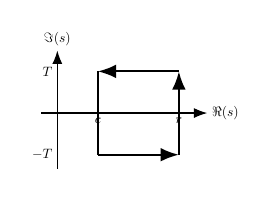
\begin{tikzpicture}[baseline={(current bounding box.center)}, scale=0.49, transform shape, >=Latex, x=1.05cm, y=0.9cm] \draw[->] (-0.4,0) -- (3.7,0) node[right] {$\Re(s)$}; \draw[->] (0,-1.6) -- (0,1.8) node[above] {$\Im(s)$}; \draw[thick, ->] (1,-1.2) -- (3,-1.2); \draw[thick, ->] (3,-1.2) -- (3,1.2); \draw[thick, ->] (3,1.2) -- (1,1.2); \draw[thick] (1,1.2) -- (1,-1.2); \node[below] at (1,0) {$c$}; \node[below] at (3,0) {$r$}; \node[left] at (0,1.2) {$T$}; \node[left] at (0,-1.2) {$-T$}; \end{tikzpicture}\)
	由 Cauchy 积分定理（Cauchy's integral theorem），由于 $y^s/s$ 在这个矩形内部没有极点，
	\(\textstyle I_c(y,\allowbreak{}T)=\allowbreak{} \frac1{2\pi i} \left( \int_{c-iT}^{r-iT} +\allowbreak{} \int_{r-iT}^{r+\allowbreak{}iT} +\allowbreak{} \int_{r+\allowbreak{}iT}^{c+\allowbreak{}iT} \right)y^s\frac{ds}{s}.\)
	于是
	\(\textstyle |I_c(y,\allowbreak{}T)| \leq\allowbreak{} \frac1{2\pi} \left( \int_c^r\frac{y^\sigma}{T}\,d\sigma +\allowbreak{} \int_{-T}^T\frac{y^r}{r}\,dt +\allowbreak{} \int_c^r\frac{y^\sigma}{T}\,d\sigma \right)\) \(\textstyle =\allowbreak{} \frac1{2\pi} \left( \frac2T\left.\frac{y^\sigma}{\log y}\right|_{\sigma=\allowbreak{}c}^r +\allowbreak{} 2T\frac{y^r}{r} \right).\)
	因为 $0<y<1$，所以
	\(\textstyle \frac{y^r}{r}\to\allowbreak{} 0,\allowbreak{} \qquad \frac{y^r}{|\log y|}\to\allowbreak{} 0\)
	当 $r\to+\infty$。因此
	\(\textstyle |I_c(y,\allowbreak{}T)| \leq\allowbreak{} \frac1{\pi T}\frac{y^c}{|\log y|}.\)

	(b) 另一方面，我们要证明
	\(\textstyle |I_c(y,\allowbreak{}T)|\leq\allowbreak{} y^c.\)
	令
	\(\textstyle R=\allowbreak{}\sqrt{c^2+\allowbreak{}T^2},\allowbreak{}\)
	并令 $C$ 为以原点为圆心、半径为 $R$ 的圆。令 $\gamma^+$ 为 $C$ 上从 $c-iT$ 出发到 $c+iT$ 结束的逆时针路径：
	\(\textstyle 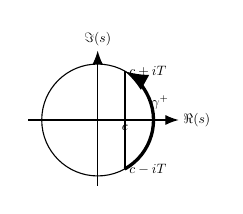
\begin{tikzpicture}[baseline={(current bounding box.center)}, scale=0.49, transform shape, >=Latex, x=1cm, y=1cm] \draw[->] (-1.8,0) -- (2.1,0) node[right] {$\Re(s)$}; \draw[->] (0,-1.7) -- (0,1.8) node[above] {$\Im(s)$}; \draw[thin] (0,0) circle (1.45); \draw[thick] (0.7,-1.27) -- (0.7,1.27); \draw[very thick, ->] (0.7,-1.27) arc[start angle=-61,end angle=61,radius=1.45]; \node[right] at (0.7,1.27) {$c+iT$}; \node[right] at (0.7,-1.27) {$c-iT$}; \node[right] at (1.28,0.45) {$\gamma^+$}; \node[below] at (0.7,0) {$c$}; \end{tikzpicture}\)
	由 Cauchy 留数定理（Cauchy residue theorem），
	\(\textstyle I_c(y,\allowbreak{}T) =\allowbreak{} \frac1{2\pi i}\int_{c-iT}^{c+\allowbreak{}iT}y^s\frac{ds}{s} =\allowbreak{} \frac1{2\pi i}\int_{\gamma^+\allowbreak{}}y^s\frac{ds}{s}.\)
	特别地，
	\(\textstyle |I_c(y,\allowbreak{}T)| \leq\allowbreak{} \frac1{2\pi}\int_{\gamma^+\allowbreak{}}\frac{y^{\Re(s)}}{|s|}\,|ds| \leq\allowbreak{} \frac1{2\pi}\cdot \frac{y^c}{R}\cdot 2\pi R \leq\allowbreak{} y^c,\allowbreak{}\)
	这里用到了 $y<1$。

	\emph{情形 2：$y>1$。} 这时考虑如下矩形：
	\(\textstyle 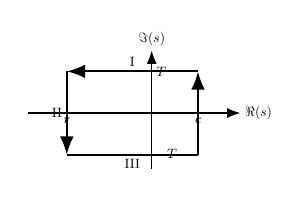
\begin{tikzpicture}[baseline={(current bounding box.center)}, scale=0.49, transform shape, >=Latex, x=1cm, y=0.9cm] \draw[->] (-3.2,0) -- (2.3,0) node[right] {$\Re(s)$}; \draw[->] (0,-1.6) -- (0,1.8) node[above] {$\Im(s)$}; \draw[thick, ->] (1.2,-1.2) -- (1.2,1.2); \draw[thick, ->] (1.2,1.2) -- (-2.2,1.2); \draw[thick, ->] (-2.2,1.2) -- (-2.2,-1.2); \draw[thick] (-2.2,-1.2) -- (1.2,-1.2); \node[below] at (1.2,0) {$c$}; \node[below] at (-2.2,0) {$r$}; \node[right] at (0,1.2) {$T$}; \node[right] at (0,-1.2) {$-T$}; \node[above] at (-0.5,1.2) {I}; \node[left] at (-2.2,0) {II}; \node[below] at (-0.5,-1.2) {III}; \end{tikzpicture}\)
	由 Cauchy 留数定理，
	\(\textstyle I_c(y,\allowbreak{}T) =\allowbreak{} \frac1{2\pi i} \left( \int_{\mathrm I} +\allowbreak{} \int_{\mathrm{II}} +\allowbreak{} \int_{\mathrm{III}} \right)y^s\frac{ds}{s} +\allowbreak{} \operatorname{Res}_{s=\allowbreak{}0}\frac{y^s}{s}.\)
	也就是说
	\(\textstyle I_c(y,\allowbreak{}T) =\allowbreak{} 1+\allowbreak{} \frac1{2\pi i} \left( \int_{\mathrm I} +\allowbreak{} \int_{\mathrm{II}} +\allowbreak{} \int_{\mathrm{III}} \right)y^s\frac{ds}{s}.\)
	和前面做同样的估计，并令 $r\to-\infty$，得到
	\(\textstyle |I_c(y,\allowbreak{}T)-1| \leq\allowbreak{} \frac{2y^c}{1+\allowbreak{}T|\log y|}.\)
	结合两种估计，即得引理。
\end{proof}

\begin{theorem}[原文 Theorem 4.10，Perron 公式]
	设 $c>0$，$x,T\geq 1$ 为实数。设 $f\in\mathcal A$，且 $L_f(s)$ 在 $s=c$ 处绝对收敛。那么对所有 $x\notin\mathbb Z$，有
	\(\textstyle \sum_{n\leq\allowbreak{} x}f(n) =\allowbreak{} \frac1{2\pi i}\int_{c-iT}^{c+\allowbreak{}iT} L_f(s)\frac{x^s}{s}\,ds +\allowbreak{} E(T),\allowbreak{}\)
	其中 $E(T)\to 0$ 当 $T\to\infty$。如果 $x\in\mathbb Z$，则公式也成立，只需把最后一项 $f(x)$ 替换为 $f(x)/2$。
\end{theorem}

\begin{proof}
	设 $x\notin\mathbb Z$。因为 $L_f(s)$ 在 $\Re(s)=c$ 上绝对收敛，所以可以交换求和与积分的次序：
	\(\textstyle \frac1{2\pi i}\int_{c-iT}^{c+\allowbreak{}iT} L_f(s)\frac{x^s}{s}\,ds\) \(\textstyle \qquad=\allowbreak{} \sum_{n\geq\allowbreak{} 1}f(n) \frac1{2\pi i} \int_{c-iT}^{c+\allowbreak{}iT}\left(\frac{x}{n}\right)^s\frac{ds}{s}.\)
	由 Lemma 4.9，
	\(\textstyle \frac1{2\pi i}\int_{c-iT}^{c+\allowbreak{}iT} L_f(s)\frac{x^s}{s}\,ds =\allowbreak{} \sum_{n\geq\allowbreak{} 1}f(n)\delta\left(\frac{x}{n}\right) +\allowbreak{} E(T),\allowbreak{}\)
	其中
	\(\textstyle |E(T)| \leq\allowbreak{} 2\sum_{n\geq\allowbreak{} 1} \frac{|f(n)|(x/n)^c} {1+\allowbreak{}T|\log(x/n)|}\) \(\textstyle =\allowbreak{} 2x^c\sum_{n\geq\allowbreak{} 1} \frac{|f(n)|}{n^c(1+\allowbreak{}T|\log(x/n)|)}.\)
	由于 $\log(x/n)\neq 0$，所以 $|E(T)|\to 0$ 当 $T\to\infty$。因此
	\(\textstyle \sum_{n\geq\allowbreak{} 1}f(n)\delta\left(\frac{x}{n}\right) =\allowbreak{} \sum_{n\leq\allowbreak{} x}f(n).\)
	$x\in\mathbb Z$ 的情形类似。
\end{proof}

\begin{remark}
	积分
	\(\textstyle \frac1{2\pi i}\int_{c-i\infty}^{c+\allowbreak{}i\infty} L_f(s)\frac{x^s}{s}\,ds\)
	通常不是绝对收敛的，这会带来问题。在实践中，我们需要一个更实用的版本。
\end{remark}

\begin{theorem}[原文 Theorem 4.11，Perron 公式的截断版本]
	设 $c>0$，$x,T\geq 1$ 为实数。设 $f\in\mathcal A$，且 $L_f(s)$ 在 $s=c$ 处绝对收敛。那么对所有 $x\notin\mathbb Z$，有
	\(\textstyle \sum_{n\leq\allowbreak{} x}f(n) =\allowbreak{} \frac1{2\pi i}\int_{c-iT}^{c+\allowbreak{}iT} L_f(s)\frac{x^s}{s}\,ds +\allowbreak{} O\left( x^c\sum_{n\geq\allowbreak{} 1} \frac{|f(n)|}{n^c(1+\allowbreak{}T|\log(x/n)|)} \right),\allowbreak{}\)
	其中误差项还满足
	\(\textstyle x^c\sum_{n\geq\allowbreak{} 1} \frac{|f(n)|}{n^c(1+\allowbreak{}T|\log(x/n)|)} \ll\allowbreak{} \frac{x^c}{T}\sum_{n\geq\allowbreak{} 1}\frac{|f(n)|}{n^c}\) \(\textstyle \quad+\allowbreak{} \left(1+\allowbreak{}\frac{x\log T}{T}\right) \max_{3x/4\leq\allowbreak{} n\leq\allowbreak{} 5x/4}|f(n)|.\)
	如果 $x\in\mathbb Z$，则公式也成立，只需把最后一项 $f(x)$ 替换为 $f(x)/2$。
\end{theorem}

\begin{proof}
	Dirichlet 级数 $L_f(s)$ 在紧区间 $[c-iT,c+iT]$ 上绝对且一致收敛。因此
	\(\textstyle \frac1{2\pi i}\int_{c-iT}^{c+\allowbreak{}iT} L_f(s)\frac{x^s}{s}\,ds =\allowbreak{} \frac1{2\pi i}\int_{c-iT}^{c+\allowbreak{}iT} \sum_{n\geq\allowbreak{} 1}\frac{f(n)}{n^s}\frac{x^s}{s}\,ds\) \(\textstyle =\allowbreak{} \sum_{n\geq\allowbreak{} 1}f(n) \frac1{2\pi i}\int_{c-iT}^{c+\allowbreak{}iT} \left(\frac{x}{n}\right)^s\frac{ds}{s}\) \(\textstyle =\allowbreak{} \sum_{n\geq\allowbreak{} 1}f(n)I_c\left(\frac{x}{n},\allowbreak{}T\right)\) \(\textstyle =\allowbreak{} \sum_{n\geq\allowbreak{} 1}f(n)\delta\left(\frac{x}{n}\right) +\allowbreak{} \sum_{n\geq\allowbreak{} 1}f(n) \left(I_c\left(\frac{x}{n},\allowbreak{}T\right) - \delta\left(\frac{x}{n}\right)\right)\) \(\textstyle =\allowbreak{} \sum_{n\leq\allowbreak{} x}^{*}f(n)+\allowbreak{}E_c(x,\allowbreak{}T).\)
	这里 $\sum_{n\leq x}^{*}$ 表示如果 $x\in\mathbb Z$，最后一项 $f(x)$ 替换为 $f(x)/2$。

	由 Lemma 4.9，
	\(\textstyle |E_c(x,\allowbreak{}T)| \leq\allowbreak{} 2\sum_{n\geq\allowbreak{} 1,\allowbreak{} n\neq\allowbreak{} x} |f(n)|\frac{(x/n)^c}{1+\allowbreak{}T|\log(x/n)|} +\allowbreak{} \frac{c}{c+\allowbreak{}T}|f(x)|,\allowbreak{}\)
	其中最后一项只在 $x\in\mathbb Z$ 时出现。因此
	\(\textstyle |E_c(x,\allowbreak{}T)| \leq\allowbreak{} 2x^c\sum_{n\geq\allowbreak{} 1,\allowbreak{} n\neq\allowbreak{} x} \frac{|f(n)|}{n^c(1+\allowbreak{}T|\log(x/n)|)} +\allowbreak{} \frac{c}{c+\allowbreak{}T}|f(x)|.\)
	特别地，
	\(\textstyle |E_c(x,\allowbreak{}T)|\to\allowbreak{} 0 \qquad (T\to\allowbreak{}\infty),\allowbreak{}\)
	于是得到 Theorem 4.10。

	现在把关于 $n$ 的和分成三部分：
	\(\textstyle \sum_{|n-x|\geq\allowbreak{} x/4}(\cdots) +\allowbreak{} \sum_{2\leq\allowbreak{} |n-x|\leq\allowbreak{} x/4}(\cdots) +\allowbreak{} \sum_{|n-x|<2}(\cdots) =\allowbreak{} E_c^{(1)}(x,\allowbreak{}T)+\allowbreak{}E_c^{(2)}(x,\allowbreak{}T)+\allowbreak{}E_c^{(3)}(x,\allowbreak{}T).\)
	对满足 $|n-x|\geq x/4$ 的项，我们使用
	\(\textstyle |\log(x/n)|\gg\allowbreak{} 1,\allowbreak{}\)
	它给出
	\(\textstyle E_c^{(1)}(x,\allowbreak{}T) \ll\allowbreak{} \sum_{|n-x|\geq\allowbreak{} x/4} \frac{x^c|f(n)|}{n^cT|\log(x/n)|} \ll\allowbreak{} \frac{x^c}{T}\sum_{n\geq\allowbreak{} 1}\frac{|f(n)|}{n^c}.\)
	对满足 $2\leq |n-x|\leq x/4$ 的项，我们有
	\(\textstyle |\log(x/n)| =\allowbreak{} \left|\log\left(1+\allowbreak{}\frac{n-x}{x}\right)\right| \gg\allowbreak{} \frac{|n-x|}{x}.\)
	所以
	\(\textstyle E_c^{(2)}(x,\allowbreak{}T) \ll\allowbreak{} \frac{x^c}{T} \sum_{2\leq\allowbreak{} |n-x|\leq\allowbreak{} x/4} \frac{|f(n)|x}{n^c|n-x|}\) \(\textstyle \ll\allowbreak{} \frac{x}{T} \left(\max_{2\leq\allowbreak{} |n-x|\leq\allowbreak{} x/4}|f(n)|\right) \sum_{2\leq\allowbreak{} |n-x|\leq\allowbreak{} x/4}\frac1{|n-x|}\) \(\textstyle \ll\allowbreak{} \frac{x\log x}{T} \max_{2\leq\allowbreak{} |n-x|\leq\allowbreak{} x/4}|f(n)|.\)
	最后，剩下的项可以平凡地估计为
	\(\textstyle E_c^{(3)}(x,\allowbreak{}T) \ll\allowbreak{} \sum_{|n-x|<2}\frac{x^c|f(n)|}{n^c} \ll\allowbreak{} \max_{|n-x|<2}|f(n)|.\)
	把这些估计相加即得定理。
\end{proof}

% compact: inserted rewritten chapters 5 and 6 from chapter5-6-rewrite.tex
% compact: extracted from ../../chapter5-6-rewrite.tex for compressed lecture only.
\chapter{指数、原根和指标}

本章始终把模 $n$ 的可逆剩余类看成群
\(
  \U n=(\Z/n\Z)^\times .
\)
所谓模 $n$ 存在原根，现代地说就是 $\U n$ 是循环群（cyclic group，循环群）；若
$g\in \U n$ 生成 $\U n$，则也称整数 $g$ 是模 $n$ 的原根。这样定义之后，后面的定理本质上都是在讨论
$\U n$ 的群结构。

\section{阶、原根与基本定理}

\begin{theorem}[二的高次幂没有原根]
若 $k\ge 3$，则模 $2^k$ 不存在原根。更准确地说，对任意奇数 $a$，有 $a^{2^{k-2}}\equiv 1\pmod {2^k}$。
\end{theorem}

\begin{proof}
先证模 $8$：任意奇数可写成 $2h+1$，而 $(2h+1)^2=4h(h+1)+1\equiv 1\pmod 8$。下面对 $k\ge3$ 归纳。$k=3$ 已证；若 $2^{k-1}\mid a^{2^{k-3}}-1$，则
$a^{2^{k-2}}-1=(a^{2^{k-3}}-1)(a^{2^{k-3}}+1)$，其中第一因子含有 $2^{k-1}$，第二因子为偶数，故乘积含有 $2^k$。于是 $a^{2^{k-2}}\equiv1\pmod {2^k}$，而 $2^{k-2}<\varphi(2^k)$，所以模 $2^k$ 没有原根。
\end{proof}

\begin{proposition}[幂的阶]
若 $(a,n)=1$，$c\ge 1$，则 $\delta_n(a^c)=\dfrac{\delta_n(a)}{(\delta_n(a),c)}$。
\end{proposition}

\begin{proposition}[互素阶的乘积]
若 $(a,n)=(b,n)=1$ 且 $(\delta_n(a),\delta_n(b))=1$，则 $\delta_n(ab)=\delta_n(a)\delta_n(b)$。
\end{proposition}

\begin{remark}
若 $\delta_n(a)$ 与 $\delta_n(b)$ 不互素，一般不能写成 $\delta_n(ab)=\operatorname{lcm}(\delta_n(a),\delta_n(b))$。例如模 $10$ 中，$3$ 与 $7$ 的阶都为 $4$，但
$3\cdot 7\equiv 1\pmod {10}$，所以乘积的阶为 $1$。
\end{remark}

\begin{theorem}[阶的最小公倍数可以实现]
若
\(
  (a,n)=(b,n)=1,
\)
则存在整数，使得
\(
  \delta_n(c)=\operatorname{lcm}(\delta_n(a),\delta_n(b)).
\)
\end{theorem}

\begin{proof}
记
\(
  r=\delta_n(a),\qquad s=\delta_n(b),\qquad L=\operatorname{lcm}(r,s),
\)
并写
\(
  L=\prod_q q^{\lambda_q}.
\)
对每个素数因子而言，在
\(
  r,\qquad s
\)
中至少有一个含有
\(
  q^{\lambda_q}.
\)
若这个最高幂来自
\(
  r,
\)
取
\(
  c_q=a^{\,r/q^{\lambda_q}};
\)
若来自
\(
  s,
\)
取
\(
  c_q=b^{\,s/q^{\lambda_q}}.
\)
于是
\(
  \delta_n(c_q)=q^{\lambda_q}.
\)
令
\(
  c=\prod_q c_q.
\)
这些阶两两互素，由上一命题可知
\(
  \delta_n(c)=\prod_q q^{\lambda_q}=L.
\)
\end{proof}

\begin{proposition}[中国剩余定理下的阶]
若
\(
  (n_1,n_2)=1,\qquad (a,n_1n_2)=1,
\)
则
\(
  \delta_{n_1n_2}(a)
  =
  \operatorname{lcm}\bigl(\delta_{n_1}(a),\delta_{n_2}(a)\bigr).
\)
\end{proposition}

\begin{proof}
由中国剩余定理（Chinese remainder theorem，中国剩余定理）
\(
  \Z/n_1n_2\Z\simeq \Z/n_1\Z\times \Z/n_2\Z
\)
可知
\(
  a^t\equiv 1\pmod {n_1n_2}
\)
当且仅当
\(
  a^t\equiv 1\pmod {n_1},\qquad
  a^t\equiv 1\pmod {n_2}.
\)
因此满足条件的正整数
\(
  t
\)
正是同时被
\(
  \delta_{n_1}(a),\qquad \delta_{n_2}(a)
\)
整除的正整数，最小者就是
\(
  \operatorname{lcm}\bigl(\delta_{n_1}(a),\delta_{n_2}(a)\bigr).
\)
\end{proof}

\begin{corollary}
若 $(n_1,n_2)=1$，且分别给定 $(a_1,n_1)=1$、$(a_2,n_2)=1$，则存在 $a$ 满足
\(
  a\equiv a_1\pmod {n_1},\qquad
  a\equiv a_2\pmod {n_2},
\)
并且
\(
  \delta_{n_1n_2}(a)
  =
  \operatorname{lcm}\bigl(\delta_{n_1}(a_1),\delta_{n_2}(a_2)\bigr).
\)
\end{corollary}

\section{原根存在定理}

为了统一表述，定义
\(
  \Phi(2^\alpha)=
  \begin{cases}
    \varphi(2^\alpha), & 0\le \alpha\le 2,\\
    \dfrac12\varphi(2^\alpha)=2^{\alpha-2}, & \alpha\ge 3.
  \end{cases}
\)
若
\(
  n=2^{\alpha_0}p_1^{\alpha_1}\cdots p_s^{\alpha_s}
\)
是 $n$ 的素因子分解，其中 $p_i$ 为奇素数，则记
\(
  \varepsilon(n)
  =
  \operatorname{lcm}\bigl(\Phi(2^{\alpha_0}),
  \varphi(p_1^{\alpha_1}),\ldots,\varphi(p_s^{\alpha_s})\bigr).
\)
这个数就是群 $\U n$ 中元素的阶所能达到的最大值，也就是 $\U n$ 的指数。

\begin{theorem}[模素数存在原根]
若 $p$ 为素数，则 $\U p$ 是循环群。等价地，存在模 $p$ 的原根。
\end{theorem}

\begin{lemma}[从模 $p$ 提升到模 $p^2$]
设 $p$ 为奇素数，$g$ 是模 $p$ 的原根。则在
\(
  g,\ g+p,\ g+2p,\ldots,g+(p-1)p
\)
中，至少有一个是模 $p^2$ 的原根。
\end{lemma}

\begin{proof}
因为每个 $g+tp$ 都模 $p$ 同余于 $g$，所以它模 $p^2$ 的阶只能是
\(
  p-1\quad\text{或}\quad p(p-1)=\varphi(p^2).
\)
如果某个 $t$ 使得
\(
  (g+tp)^{p-1}\not\equiv 1\pmod {p^2},
\)
那么 $g+tp$ 就是模 $p^2$ 的原根。

设
\(
  g^{p-1}=1+cp.
\)
用二项式展开得
\(
  (g+tp)^{p-1}
  \equiv
  g^{p-1}+(p-1)g^{p-2}tp
  \equiv
  1+p\bigl(c+(p-1)g^{p-2}t\bigr)
  \pmod {p^2}.
\)
括号中关于 $t$ 的一次式模 $p$ 只有一个零点。因此在 $t=0,1,\ldots,p-1$ 中，至多一个 $t$ 使得
$(g+tp)^{p-1}\equiv 1\pmod {p^2}$。于是至少存在一个 $t$ 使 $g+tp$ 为模 $p^2$ 原根。
\end{proof}

\begin{theorem}[奇素数幂模原根]
若 $p$ 为奇素数，$\alpha\ge 1$，则模 $p^\alpha$ 存在原根。更具体地，若 $g$ 是模 $p^2$ 的原根，则 $g$ 是每个模
$p^\alpha$ 的原根。
\end{theorem}

\begin{proof}
对 $\alpha=1,2$ 已由前面的定理与引理得到。设 $\alpha\ge 2$，并假设 $g$ 是模 $p^\alpha$ 的原根，即
\(
  \delta_{p^\alpha}(g)=\varphi(p^\alpha)=p^{\alpha-1}(p-1).
\)
因为 $g^{\varphi(p^\alpha)}\equiv 1\pmod {p^\alpha}$，可写
\(
  g^{\varphi(p^\alpha)}=1+up^\alpha.
\)
若 $p\nmid u$，则
\(
  g^{\varphi(p^\alpha)}\not\equiv 1\pmod {p^{\alpha+1}},
\)
从而模 $p^{\alpha+1}$ 的阶为 $p\varphi(p^\alpha)=\varphi(p^{\alpha+1})$。

只需说明从模 $p^2$ 原根开始，始终有 $p\nmid u$。若某一步 $p\mid u$，则
\(
  g^{\varphi(p^\alpha)}\equiv 1\pmod {p^{\alpha+1}}.
\)
降到模 $p^2$ 后会推出
\(
  g^{p-1}\equiv 1\pmod {p^2},
\)
这与 $g$ 为模 $p^2$ 原根矛盾。因此 $g$ 的阶每一步都乘以 $p$，故 $g$ 是所有模 $p^\alpha$ 的原根。
\end{proof}

\begin{corollary}
若 $p$ 为奇素数，$\alpha\ge 1$，则模 $2p^\alpha$ 也存在原根。
\end{corollary}

\begin{proof}
由中国剩余定理，具体映射为
\(\Phi:\U{2p^\alpha}\to \U{2}\times\U{p^\alpha},\ [a]_{2p^\alpha}\mapsto ([a]_2,[a]_{p^\alpha})\)。
由于 \(\U{2}=\{[1]_2\}\)，复合第二个分量投影得到同构
\(\pi:\U{2p^\alpha}\to \U{p^\alpha},\ [a]_{2p^\alpha}\mapsto [a]_{p^\alpha}\)。
其反向映射为：给定 \([u]_{p^\alpha}\in\U{p^\alpha}\)，取唯一的 \([x]_{2p^\alpha}\) 满足
\(x\equiv 1\pmod 2,\ x\equiv u\pmod {p^\alpha}\)，并令
\(\iota([u]_{p^\alpha})=[x]_{2p^\alpha}\)。因此若 \([g]_{p^\alpha}\) 是生成元，则 \(\iota([g]_{p^\alpha})\) 是 \(\U{2p^\alpha}\) 的生成元，即给出模 \(2p^\alpha\) 的原根。
\end{proof}

\begin{theorem}[原根存在的完全判别]
模 $n$ 存在原根当且仅当
\(
  n=1,\ 2,\ 4,\ p^\alpha,\ 2p^\alpha
\)
之一，其中 $p$ 为奇素数，$\alpha\ge 1$。
\end{theorem}

\begin{proof}
充分性已经证明：$1,2,4$ 的情形直接；奇素数幂与其二倍由上面的定理和推论得到。

下面证明必要性。若 $2^\alpha\mid n$ 且 $\alpha\ge 3$，则由中国剩余定理，$\U n$ 映到 $\U{2^\alpha}$。模
$2^\alpha$ 中任意元素的阶都整除 $2^{\alpha-2}$，而 $\varphi(2^\alpha)=2^{\alpha-1}$，这会使 $\U n$ 的指数严格小于
$\varphi(n)$，故 $\U n$ 不能循环。

若 $n$ 含有两个不同的奇素因子，即
\(
  p^\alpha q^\beta\mid n,\qquad p\ne q,
\)
则
\(
  \varphi(p^\alpha)\quad\text{和}\quad \varphi(q^\beta)
\)
都为偶数。中国剩余定理给出
\(
  \U n
  \longrightarrow
  \U{p^\alpha}\times \U{q^\beta}
\)
的投影，而右边元素的阶所能达到的最大值只可能是
\(
  \operatorname{lcm}\bigl(\varphi(p^\alpha),\varphi(q^\beta)\bigr)
  <
  \varphi(p^\alpha)\varphi(q^\beta).
\)
因此整体群的指数小于群的阶，也不可能循环。

于是 $n$ 至多含一个奇素因子，且 $2$ 的指数至多为 $1$，除非没有奇素因子时允许 $2,4$。这正得到列出的形式。
\end{proof}

\begin{theorem}[循环情形中给定阶的元素个数]
若模 $n$ 存在原根，且 $d\mid \varphi(n)$，则模 $n$ 中阶为 $d$ 的元素恰有
\(
  \varphi(d)
\)
个。特别地，模 $n$ 的原根个数为
\(
  \varphi(\varphi(n)).
\)
\end{theorem}

\begin{proof}
设 $g$ 是模 $n$ 的原根，则 $\U n=\langle g\rangle$，群的阶为 $m=\varphi(n)$。任意元素可唯一写成
\(
  g^r,\qquad r\in \Z/m\Z.
\)
由幂的阶公式，
\(
  \delta_n(g^r)=\frac{m}{(m,r)}.
\)
令它等于 $d$，即
\(
  (m,r)=m/d.
\)
这等价于 $r=(m/d)u$ 且 $(u,d)=1$。这样的 $u$ 模 $d$ 有 $\varphi(d)$ 个。
\end{proof}

\begin{theorem}[一般模数中给定阶的元素个数]
设 \(n=2^{\alpha_0}p_1^{\alpha_1}\cdots p_s^{\alpha_s}\)，其中 \(p_i\) 为互异奇素数。若 \(d\mid \varepsilon(n)\)，则 \(\U n\) 中阶为 \(d\) 的元素个数为
\(
A_n(d)=\sum_{e\mid d}\mu\!\left(\frac d e\right)\rho_{\alpha_0}(e)\prod_{i=1}^s (e,\varphi(p_i^{\alpha_i})),
\)
其中 \(\mu\) 是 Möbius 函数（Möbius function），并且 \(\rho_{\alpha}(e)=1\) 当 \(\alpha=0,1\)，\(\rho_2(e)=(e,2)\)，而 \(\alpha\ge3\) 时 \(\rho_{\alpha}(e)=(e,2)(e,2^{\alpha-2})\)。若 \(d\nmid\varepsilon(n)\)，则这样的元素不存在。
\end{theorem}

\begin{proof}
记 \(R_n(e)=\#\{x\in\U n:x^e=1\}\)。由中国剩余定理，\(\U n\simeq \U{2^{\alpha_0}}\times \prod_{i=1}^s\U{p_i^{\alpha_i}}\)。奇素数幂部分是循环群，故 \(\U{p_i^{\alpha_i}}\) 中满足 \(x^e=1\) 的元素个数为 \((e,\varphi(p_i^{\alpha_i}))\)。二幂部分中，\(\alpha=0,1\) 时群平凡，\(\alpha=2\) 时 \(\U4\simeq C_2\)，\(\alpha\ge3\) 时 \(\U{2^\alpha}\simeq C_2\times C_{2^{\alpha-2}}\)，所以二幂部分贡献正是 \(\rho_{\alpha_0}(e)\)。因此 \(R_n(e)=\rho_{\alpha_0}(e)\prod_{i=1}^s(e,\varphi(p_i^{\alpha_i}))\)。若 \(A_n(t)\) 表示阶恰为 \(t\) 的元素个数，则 \(R_n(e)=\sum_{t\mid e}A_n(t)\)，因为 \(x^e=1\) 当且仅当 \(x\) 的阶整除 \(e\)。由 Möbius 反演（Möbius inversion）得到所述公式。最后，元素的阶必整除群的指数 \(\varepsilon(n)\)，所以 \(d\nmid\varepsilon(n)\) 时不存在阶为 \(d\) 的元素。
\end{proof}

\section{结构定理、指标与指标组}

上节讨论原根是否存在。本节把剩余类群的结构直接写出来。这样做之后，“原根存在”只是“这些直积分量能否合并成一个循环群”的特例。

\begin{theorem}[奇素数幂模单位群]
若 $p$ 为奇素数，$\alpha\ge 1$，取模 $p^\alpha$ 的原根 $g$，则映射
\(
  \Cyc{\varphi(p^\alpha)}
  \longrightarrow
  \U{p^\alpha},\qquad
  r\longmapsto g^r
\)
是群同构。
\end{theorem}

\begin{theorem}[二的幂模单位群]
若 $\alpha\ge 3$，则
\(
  \U{2^\alpha}\simeq \Cyc2\times \Cyc{2^{\alpha-2}}.
\)
具体地，映射
\(
  \Cyc2\times \Cyc{2^{\alpha-2}}
  \longrightarrow
  \U{2^\alpha},\qquad
  (u,v)\longmapsto (-1)^u5^v
\)
是群同构。也可以把 $5$ 换成 $3$；此时 $3$ 在第二个因子中也生成一个阶为 $2^{\alpha-2}$ 的循环子群。
\end{theorem}

\begin{proof}
先证明 $5$ 的阶为 $2^{\alpha-2}$。由二项式展开可归纳得到
\(
  5^{2^r}\equiv 1+2^{r+2}\pmod {2^{r+3}}\qquad(r\ge 0).
\)
因此 $5^{2^{\alpha-2}}\equiv 1\pmod {2^\alpha}$，但
$5^{2^{\alpha-3}}\not\equiv 1\pmod {2^\alpha}$，所以
\(
  \delta_{2^\alpha}(5)=2^{\alpha-2}.
\)

接着说明每个奇数类都唯一写成 $(-1)^u5^v$。集合
\(
  \{5^v:0\le v<2^{\alpha-2}\}
\)
全部同余于 $1\pmod 4$；而
\(
  \{-5^v:0\le v<2^{\alpha-2}\}
\)
全部同余于 $-1\pmod 4$。这两个集合不相交，总共有
$2\cdot 2^{\alpha-2}=2^{\alpha-1}=\varphi(2^\alpha)$ 个元素，因此正好给出全部奇剩余类。唯一性也随之成立。
\end{proof}

\begin{theorem}[一般结构定理]
设
\(
  n=2^{\alpha_0}p_1^{\alpha_1}\cdots p_s^{\alpha_s},
\)
其中 $p_i$ 为两两不同的奇素数。对每个 $i$ 取模 $p_i^{\alpha_i}$ 的原根 $g_i$。则
\(
  \U n
  \simeq
  \U{2^{\alpha_0}}
  \times
  \U{p_1^{\alpha_1}}
  \times\cdots\times
  \U{p_s^{\alpha_s}}.
\)
这里的同构由中国剩余定理给出：
\(
  a\pmod n
  \longmapsto
  \bigl(a\bmod 2^{\alpha_0},\ a\bmod p_1^{\alpha_1},\ldots,a\bmod p_s^{\alpha_s}\bigr).
\)
反向映射是唯一满足
\(
  a\equiv a_0\pmod {2^{\alpha_0}},\qquad
  a\equiv a_i\pmod {p_i^{\alpha_i}}\quad(1\le i\le s)
\)
的剩余类 $a\pmod n$。
\end{theorem}

\begin{proof}
这是中国剩余定理在单位群上的限制。因为一个类模 $n$ 可逆，当且仅当它在每个素数幂模数下都可逆，所以环同构限制为单位群同构。
\end{proof}

把局部同构写开，可得到完全显式的坐标表示：若 $\alpha_0=0$，没有二次因子坐标；若 $\alpha_0=1$，$\U2$ 为平凡群，也没有有效坐标；若 $\alpha_0=2$，$\U4=\{\pm1\}$，用一个坐标 $u\in\Cyc2$ 表示 $(-1)^u$；若 $\alpha_0\ge3$，用两个坐标 \(u\in\Cyc2,\ v\in\Cyc{2^{\alpha_0-2}}\) 表示 \((-1)^u5^v\pmod {2^{\alpha_0}}\)；对每个奇素数幂 $p_i^{\alpha_i}$，用坐标 \(r_i\in \Cyc{\varphi(p_i^{\alpha_i})}\) 表示 \(g_i^{r_i}\pmod {p_i^{\alpha_i}}\)。因此在这些坐标下，群运算就是各坐标相加。这是后面“指标组”的来源。

\begin{definition}[指标]
若模 $n$ 存在原根 $g$，对任意 $(a,n)=1$，唯一的
\(
  r\in \Z/\varphi(n)\Z
\)
使
\(
  g^r\equiv a\pmod n
\)
成立。这个 $r$ 称为 $a$ 以 $g$ 为底的指标（index，指标），记为
\(
  \operatorname{ind}_g a\equiv r\pmod{\varphi(n)}.
\)
\end{definition}

\begin{proposition}[指标的基本性质]
设 $g$ 是模 $n$ 的原根，$(a,n)=(b,n)=1$。则
\(
  \operatorname{ind}_g(ab)
  \equiv
  \operatorname{ind}_g a+\operatorname{ind}_g b
  \pmod{\varphi(n)}.
\)
并且
\(
  \delta_n(a)
  =
  \frac{\varphi(n)}
  {(\varphi(n),\operatorname{ind}_g a)}.
\)
\end{proposition}

\begin{proof}
若 $a\equiv g^r$、$b\equiv g^s$，则 $ab\equiv g^{r+s}$，这给出指标的加法公式。阶公式则由
\(
  \delta_n(g^r)=\frac{\delta_n(g)}{(\delta_n(g),r)}
  =
  \frac{\varphi(n)}{(\varphi(n),r)}
\)
直接得到。
\end{proof}

\begin{proposition}[换底公式]
若 $g_1,g_2$ 都是模 $n$ 的原根，则
\(
  \operatorname{ind}_{g_1}g_2\cdot \operatorname{ind}_{g_2}g_1
  \equiv 1\pmod{\varphi(n)}.
\)
并且对任意 $(a,n)=1$，
\(
  \operatorname{ind}_{g_1}a
  \equiv
  \operatorname{ind}_{g_1}g_2\cdot \operatorname{ind}_{g_2}a
  \pmod{\varphi(n)}.
\)
\end{proposition}

\begin{proof}
设 $g_2\equiv g_1^u$，$g_1\equiv g_2^v$。代入得到
\(
  g_1\equiv (g_1^u)^v=g_1^{uv}\pmod n.
\)
因为 $g_1$ 的阶为 $\varphi(n)$，所以 $uv\equiv1\pmod{\varphi(n)}$。
若 $a\equiv g_2^r$，则
\(
  a\equiv (g_1^u)^r=g_1^{ur}\pmod n,
\)
即得到第二个公式。
\end{proof}

\begin{definition}[指标组]
若模 $n$ 不一定存在原根，就用上一节结构定理给出的坐标来代替单一指标。设
\(
  n=2^{\alpha_0}p_1^{\alpha_1}\cdots p_s^{\alpha_s}.
\)
对奇素数幂部分，取原根 $g_i$，令
\(
  r_i=\operatorname{ind}_{g_i}(a\bmod p_i^{\alpha_i})
  \in \Cyc{\varphi(p_i^{\alpha_i})}.
\)
对二的幂部分，若 $\alpha_0\ge3$，唯一写
\(
  a\equiv (-1)^{r_{-1}}5^{r_5}\pmod {2^{\alpha_0}},
  \qquad
  r_{-1}\in\Cyc2,\quad r_5\in \Cyc{2^{\alpha_0-2}}.
\)
把这些坐标合在一起，称为 $a$ 的指标组（index group coordinates，指标组坐标）。
\end{definition}

在指标组中，乘法变成坐标加法。例如当 $\alpha\ge3$ 时，
\(
  a\equiv (-1)^{r_{-1}(a)}5^{r_5(a)},\qquad
  b\equiv (-1)^{r_{-1}(b)}5^{r_5(b)}
  \pmod {2^\alpha}
\)
蕴含
\(
  r_{-1}(ab)\equiv r_{-1}(a)+r_{-1}(b)\pmod 2,
\)
\(
  r_5(ab)\equiv r_5(a)+r_5(b)\pmod {2^{\alpha-2}}.
\)
这正是手写稿中“指标组”的含义：用一个或多个循环坐标记录单位群元素。

\section{二项同余方程与 $k$ 次剩余}

所谓二项同余方程，就是
\(
  x^k\equiv a\pmod n,\qquad (a,n)=1.
\)
在群论语言中，它就是询问 $a$ 是否属于群 $\U n$ 中的 $k$ 次幂像。

\begin{theorem}[循环情形的判别]
假设模 $n$ 存在原根 $g$，令
\(
  m=\varphi(n),\qquad r=\operatorname{ind}_g a.
\)
则同余方程
\(
  x^k\equiv a\pmod n
\)
有解当且仅当
\(
  (k,m)\mid r.
\)
若有解，则解的个数为
\(
  (k,m).
\)
\end{theorem}

\begin{proof}
写 $x\equiv g^y$。方程等价于
\(
  g^{ky}\equiv g^r\pmod n,
\)
即
\(
  ky\equiv r\pmod m.
\)
这是一个一次同余。它有解当且仅当 $(k,m)\mid r$；有解时模 $m$ 的解数为 $(k,m)$。
\end{proof}

\begin{corollary}[循环情形的指数判别]
在上一定理的假设下，$a$ 是模 $n$ 的 $k$ 次剩余当且仅当
\(
  a^{\,\varphi(n)/(k,\varphi(n))}\equiv 1\pmod n.
\)
模 $n$ 的 $k$ 次剩余个数为
\(
  \frac{\varphi(n)}{(k,\varphi(n))}.
\)
\end{corollary}

\begin{proof}
令 $m=\varphi(n)$，$r=\operatorname{ind}_g a$。条件 $(k,m)\mid r$ 等价于
\(
  \frac{m}{(k,m)}r\equiv 0\pmod m,
\)
也就是
\(
  (g^r)^{m/(k,m)}\equiv 1\pmod n.
\)
而满足 $(k,m)\mid r$ 的 $r\in\Z/m\Z$ 恰有 $m/(k,m)$ 个。
\end{proof}

\begin{theorem}[模 $2^\alpha$ 的二项同余]
设 $\alpha\ge3$，$a$ 为奇数，并写
\(
  a\equiv (-1)^{r_{-1}}5^{r_5}\pmod {2^\alpha},
  \qquad
  r_{-1}\in\Cyc2,\quad r_5\in\Cyc{2^{\alpha-2}}.
\)
则
\(
  x^k\equiv a\pmod {2^\alpha}
\)
的可解性如下：

\begin{enumerate}[label=(\roman*),leftmargin=*]
  \item 若 $k$ 为奇数，则方程总有唯一解。
  \item 若 $k$ 为偶数，则方程有解当且仅当
  \(
    r_{-1}=0,\qquad
    (k,2^{\alpha-2})\mid r_5.
  \)
  有解时，解数为
  \(
    2\,(k,2^{\alpha-2}).
  \)
\end{enumerate}
\end{theorem}

\begin{proof}
写
\(
  x\equiv (-1)^u5^v\pmod {2^\alpha}.
\)
方程 $x^k\equiv a$ 等价于指标组中的两个同余：
\(
  ku\equiv r_{-1}\pmod 2,\qquad
  kv\equiv r_5\pmod {2^{\alpha-2}}.
\)
若 $k$ 为奇数，乘以 $k$ 在两个循环群上都是自同构，因此唯一可解。
若 $k$ 为偶数，则第一个同余变成 $0\equiv r_{-1}\pmod2$，所以必须 $r_{-1}=0$；此时 $u$ 有两个选择。第二个同余有解当且仅当
$(k,2^{\alpha-2})\mid r_5$，有解时 $v$ 有 $(k,2^{\alpha-2})$ 个选择。乘起来得到解数。
\end{proof}

\begin{theorem}[一般模数的二项同余]
设
\(
  n=2^{\alpha_0}p_1^{\alpha_1}\cdots p_s^{\alpha_s}.
\)
则
\(
  x^k\equiv a\pmod n
\)
有解当且仅当它在每个局部模数
\(
  2^{\alpha_0},\quad p_1^{\alpha_1},\ldots,p_s^{\alpha_s}
\)
下都有解。若有解，则总解数等于各局部解数之积。
\end{theorem}

\begin{proof}
中国剩余定理给出
\(
  \Z/n\Z\simeq
  \Z/2^{\alpha_0}\Z\times
  \Z/p_1^{\alpha_1}\Z\times\cdots\times
  \Z/p_s^{\alpha_s}\Z.
\)
在这个同构下，方程 $x^k=a$ 逐坐标成立。因此整体可解性等价于每个局部方程可解；整体解由局部解唯一拼接，所以解数相乘。
\end{proof}

\chapter{Dirichlet 特征}

\section{有限 Abel 群的特征}

\begin{definition}
设 $G$ 为有限 Abel 群（finite Abelian group，有限 Abel 群）。一个群同态
\(
  \chi:G\longrightarrow \C^\times
\)
称为 $G$ 的一个特征（character，特征）。由于 $G$ 有限，$\chi(g)$ 都是单位根，所以也可把值域看成
\(
  S^1=\{z\in\C:|z|=1\}.
\)
所有特征在逐点乘法下构成群，记为
\(
  G^\vee=\Hom(G,\C^\times),
\)
称为 $G$ 的特征群（character group，特征群）。
\end{definition}

\begin{example}
若 $G=\Cyc m$，则每个特征由 $1\in\Cyc m$ 的像决定。对
$j\in\Z/m\Z$，定义
\(
  \chi_j(r)=\expi{jr/m}\qquad(r\in\Z/m\Z).
\)
则
\(
  (\Cyc m)^\vee=\{\chi_j:j\in\Z/m\Z\},
\)
并且 $j\mapsto \chi_j$ 给出
\(
  \Cyc m\simeq (\Cyc m)^\vee.
\)
\end{example}

\begin{theorem}[直积的对偶群]
设 $G,H$ 为有限 Abel 群。则映射
\(\Phi:G^\vee\times H^\vee\longrightarrow (G\times H)^\vee,\quad
(\chi,\psi)\longmapsto\bigl((g,h)\mapsto \chi(g)\psi(h)\bigr)\)
是群同构。它的逆映射为
\(\Psi:(G\times H)^\vee\longrightarrow G^\vee\times H^\vee,\quad
\eta\longmapsto(\eta_G,\eta_H)\)，其中
\(\eta_G(g)=\eta(g,1_H)\)，\(\eta_H(h)=\eta(1_G,h)\)。
\end{theorem}

\begin{proof}
先看 \(\Phi\)。若 \(\chi\in G^\vee\)、\(\psi\in H^\vee\)，则 \((g,h)\mapsto \chi(g)\psi(h)\) 是 \(G\times H\) 到 \(\C^\times\) 的群同态，所以 \(\Phi\) 定义良好，并且显然保持逐点乘法。

再看 \(\Psi\)。若 \(\eta\in (G\times H)^\vee\)，则 \(g\mapsto\eta(g,1_H)\) 是 \(G\) 的特征，\(h\mapsto\eta(1_G,h)\) 是 \(H\) 的特征，所以 \(\Psi\) 也定义良好。对任意 \(\eta\in (G\times H)^\vee\)，因为 \((g,h)=(g,1_H)(1_G,h)\)，所以 \(\eta(g,h)=\eta(g,1_H)\eta(1_G,h)=\eta_G(g)\eta_H(h)\)，即 \(\Phi(\Psi(\eta))=\eta\)。另一方面，若从 \((\chi,\psi)\) 出发，则 \(\Psi(\Phi(\chi,\psi))=(\chi,\psi)\)。因此 \(\Phi\) 是同构，逆映射就是 \(\Psi\)。
\end{proof}

\begin{theorem}[有限 Abel 群的对偶]
若 $G$ 为有限 Abel 群，则
\(
  G^\vee\simeq G.
\)
更自然地说，求值映射
\(
  G\longrightarrow G^{\vee\vee},\qquad
  a\longmapsto\bigl(\chi\mapsto \chi(a)\bigr)
\)
是典范同构。
\end{theorem}

\begin{proof}
有限 Abel 群可分解为循环群直积：
\(
  G\simeq \Cyc{m_1}\times\cdots\times \Cyc{m_r}.
\)
由上一定理，直积的特征群等于各因子的特征群之积：
\(
  G^\vee\simeq
  (\Cyc{m_1})^\vee\times\cdots\times(\Cyc{m_r})^\vee.
\)
每个循环因子都有
\(
  (\Cyc{m_i})^\vee\simeq \Cyc{m_i},
\)
所以 $G^\vee\simeq G$。再对 $G^\vee$ 应用同样结论，并注意求值映射在每个循环因子上就是
\(
  r\longmapsto(\chi_j\mapsto \expi{jr/m}),
\)
可见它是同构。
\end{proof}

\begin{theorem}[特征的正交关系]
设 $G$ 为有限 Abel 群，$\chi,\psi\in G^\vee$。则
\(
  \sum_{a\in G}\chi(a)\psi^{-1}(a)
  =
  \begin{cases}
    |G|,& \chi=\psi,\\
    0,& \chi\ne\psi.
  \end{cases}
\)
这里 \(\psi^{-1}\) 表示 \(G^\vee\) 中 \(\psi\) 的逆特征；由于特征取值为单位根，\(\psi^{-1}(a)=\psi(a)^{-1}=\overline{\psi(a)}=\psi(a^{-1})\)。特别地，取 \(\psi=1\)，得到
\(
  \sum_{a\in G}\chi(a)
  =
  \begin{cases}
    |G|,& \chi=1,\\
    0,& \chi\ne1.
  \end{cases}
\)
并且对任意 \(g,h\in G\)，有与上式对偶的正交关系
\(
  \sum_{\chi\in G^\vee}\chi(g)\chi(h^{-1})
  =
  \begin{cases}
    |G|,& g=h,\\
    0,& g\ne h.
  \end{cases}
\)
特别地，取 \(h=1\)，得到
\(
  \sum_{\chi\in G^\vee}\chi(g)
  =
  \begin{cases}
    |G|,& g=1,\\
    0,& g\ne1.
  \end{cases}
\)
\end{theorem}

\begin{proof}
第一式中若 $\chi=\psi$，每项为 $1$。若 $\chi\ne\psi$，令
\(
  \eta=\chi\psi^{-1}.
\)
则 $\eta$ 是非平凡特征。取 $b\in G$ 使 $\eta(b)\ne1$，记
\(
  S=\sum_{a\in G}\eta(a).
\)
乘以 $\eta(b)$ 后
\(
  \eta(b)S=\sum_{a\in G}\eta(ba)=\sum_{a\in G}\eta(a)=S,
\)
故 $(\eta(b)-1)S=0$，所以 $S=0$。

对偶正交关系也可直接证明。若 \(g\ne h\)，则 \(gh^{-1}\ne1\)，由
$G\simeq G^{\vee\vee}$ 可知存在 $\chi_0$ 使 $\chi_0(gh^{-1})\ne1$。令
\(
  T=\sum_{\chi\in G^\vee}\chi(g)\chi(h^{-1}).
\)
则
\(
  \chi_0(gh^{-1})T
  =
  \sum_{\chi\in G^\vee}(\chi_0\chi)(g)(\chi_0\chi)(h^{-1})
  =
  T,
\)
故 $T=0$。若 \(g=h\)，每项为 \(1\)。两个特例分别由第一式取 \(\psi=1\) 和对偶式取 \(h=1\) 得到。
\end{proof}

\section{Dirichlet 特征的定义与正交关系}

\begin{definition}
设 $N\ge1$。模 $N$ 的 Dirichlet 特征（Dirichlet character，Dirichlet 特征）是群
\(
  \U N
\)
的特征
\(
  \chi:\U N\longrightarrow \C^\times
\)
延拓到整数上的函数：若 $(a,N)=1$，则 $\chi(a)$ 只由 $a\bmod N$ 决定；若 $(a,N)>1$，则规定
\(
  \chi(a)=0.
\)
\end{definition}

因此 Dirichlet 特征满足：
\(
  \chi(a+N)=\chi(a),\qquad
  \chi(ab)=\chi(a)\chi(b),\qquad
  \chi(1)=1.
\)
这里第二个等式对所有整数 $a,b$ 成立；若某个数与 $N$ 不互素，两边都按上面的零值规则理解。

\begin{definition}
模 $N$ 的主特征（principal character，主特征）记为 $\chi_0$，定义为
\(
  \chi_0(a)=
  \begin{cases}
    1,&(a,N)=1,\\
    0,&(a,N)>1.
  \end{cases}
\)
\end{definition}

\begin{proposition}
模 $N$ 的 Dirichlet 特征共有 $\varphi(N)$ 个，并且它们构成群 $(\U N)^\vee$。
\end{proposition}

\begin{proof}
这是有限 Abel 群 $\U N$ 的特征群。因为
\(
  |(\U N)^\vee|=|\U N|=\varphi(N),
\)
所以模 $N$ 的 Dirichlet 特征共有 $\varphi(N)$ 个。
\end{proof}

\begin{theorem}[Dirichlet 特征的正交关系]
设 $\chi$ 遍历模 $N$ 的所有 Dirichlet 特征。若 $(a,N)=1$，则
\(
  \sum_{\chi\bmod N}\chi(a)
  =
  \begin{cases}
    \varphi(N),& a\equiv 1\pmod N,\\
    0,& a\not\equiv 1\pmod N.
  \end{cases}
\)
若 $\chi,\psi$ 为模 $N$ 的特征，则
\(
  \sum_{a\bmod N,\allowbreak{}(a,N)=1}
  \chi(a)\overline{\psi(a)}
  =
  \begin{cases}
    \varphi(N),& \chi=\psi,\\
    0,& \chi\ne\psi.
  \end{cases}
\)
\end{theorem}

\begin{proof}
这就是上一节有限 Abel 群正交关系在
\(
  G=\U N
\)
上的直接应用。注意求和只在可逆剩余类上进行；延拓到非互素整数时特征值为 $0$。
\end{proof}

\section{本原特征与导子}

\begin{definition}
设 $\chi$ 是模 $N$ 的 Dirichlet 特征。若存在真因子 $d\mid N$，$d<N$，以及模 $d$ 的特征 $\chi^\ast$，使得对所有整数 $a$，
\(
  \chi(a)=\chi^\ast(a)\chi_0^{(N)}(a),
\)
即当 $(a,N)=1$ 时
\(
  \chi(a)=\chi^\ast(a),
\)
则称 $\chi$ 由模 $d$ 的特征提升而来。若不存在这样的真因子 $d$，则称 $\chi$ 是本原特征（primitive character，本原特征）。

使 $\chi$ 可由模 $d$ 的特征提升而来的最小正整数 $d$，称为 $\chi$ 的导子（conductor，导子），记为
\(
  \cond(\chi).
\)
\end{definition}

\begin{lemma}[降模判别]
设 \(\chi\) 是模 \(N\) 的 Dirichlet 特征，且 \(d\mid N\)。则以下三个条件等价：
\begin{enumerate}[label=(\alph*)]
  \item 存在模 \(d\) 的 Dirichlet 特征 \(\chi'\)，使得当 \((a,N)=1\) 时有 \(\chi(a)=\chi'(a)\)；
  \item 若 \((a,N)=1\) 且 \(a\equiv1\pmod d\)，则 \(\chi(a)=1\)；
  \item 若 \((a,N)=(a',N)=1\) 且 \(a\equiv a'\pmod d\)，则 \(\chi(a)=\chi(a')\)。
\end{enumerate}
\end{lemma}

\begin{proof}
\((a)\Rightarrow(b)\Rightarrow(c)\) 是直接的。只证 \((c)\Rightarrow(a)\)。先说明：若 \((a,d)=1\)，则可取 \(A\in\Z\) 满足 \(A\equiv a\pmod d\) 且 \((A,N)=1\)。事实上令 \(q=\prod_{p\mid N,\ p\nmid ad}p\)，空积时取 \(q=1\)，并取 \(A=a+qd\)。对任意 \(p\mid N\)：若 \(p\mid d\)，则 \(p\nmid a\)，故 \(A\equiv a\not\equiv0\pmod p\)；若 \(p\nmid d\) 且 \(p\nmid a\)，则 \(p\mid q\)，故 \(A\equiv a\not\equiv0\pmod p\)；若 \(p\nmid d\) 且 \(p\mid a\)，则 \(p\nmid qd\)，故 \(A\equiv qd\not\equiv0\pmod p\)。所以 \((A,N)=1\)。

现在定义模 \(d\) 上的函数 \(\chi'\)：若 \((a,d)>1\)，令 \(\chi'(a)=0\)；若 \((a,d)=1\)，取上述 \(A\equiv a\pmod d\)、\((A,N)=1\)，令 \(\chi'(a)=\chi(A)\)。若 \(A,B\) 是两个这样的选择，则 \(A\equiv B\pmod d\) 且 \((A,N)=(B,N)=1\)，由 \((c)\) 得 \(\chi(A)=\chi(B)\)，所以 \(\chi'\) 定义良好。它显然只依赖于 \(a\bmod d\)。若 \((a,d)=(b,d)=1\)，取提升 \(A,B\)；再取 \(C\equiv ab\pmod d\)、\((C,N)=1\)，则 \(C\equiv AB\pmod d\)，由 \((c)\) 得 \(\chi'(ab)=\chi(C)=\chi(AB)=\chi(A)\chi(B)=\chi'(a)\chi'(b)\)。若 \(a\) 或 \(b\) 与 \(d\) 不互素，乘法两边都为 \(0\)。因此 \(\chi'\) 是模 \(d\) 的 Dirichlet 特征。最后，当 \((a,N)=1\) 时，可在定义中直接取 \(A=a\)，于是 \(\chi'(a)=\chi(a)\)，即 \(\chi\) 由模 \(d\) 的特征提升而来。
\end{proof}

\begin{theorem}[导子的基本刻画]
设 $\chi$ 是模 $N$ 的 Dirichlet 特征。则存在唯一的本原特征 $\chi^\ast$，其模数为
\(
  d=\cond(\chi),
\)
使得当 $(a,N)=1$ 时
\(
  \chi(a)=\chi^\ast(a).
\)
换言之，$\chi$ 是从唯一的本原特征 $\chi^\ast\bmod d$ 提升到模 $N$ 的。
\end{theorem}

\begin{proof}
令 $d$ 为所有可提升模数中的最小者。若对应的 $\chi^\ast\bmod d$ 仍然不是本原的，则它又可由某个真因子 $d'<d$ 的特征提升而来，于是 $\chi$ 也可由模 $d'$ 的特征提升而来，矛盾。因此 $\chi^\ast$ 本原。

唯一性来自可逆类上的一致性：若两个本原特征 $\chi_1\bmod d_1$、$\chi_2\bmod d_2$ 都诱导出 $\chi\bmod N$，则 $\chi$ 可由模
$(d_1,d_2)$ 上的特征诱导。由 $d_1,d_2$ 的最小性得到 $d_1=d_2$，再由可逆类上的取值相同得到特征相同。
\end{proof}

\begin{theorem}[中国剩余定理下的分解]
设
\(
  N=\prod_{i=1}^s p_i^{\alpha_i}.
\)
则
\(
  \U N\simeq \prod_{i=1}^s \U{p_i^{\alpha_i}},
\)
从而每个模 $N$ 的特征可唯一写成
\(
  \chi=\prod_{i=1}^s\chi_i,
\)
其中 $\chi_i$ 是模 $p_i^{\alpha_i}$ 的特征，并按中国剩余定理拉回到模 $N$。并且
\(
  \cond(\chi)=\prod_{i=1}^s \cond(\chi_i).
\)
特别地，$\chi\bmod N$ 本原当且仅当每个 $\chi_i\bmod p_i^{\alpha_i}$ 都本原。
\end{theorem}

\begin{proof}
中国剩余定理给出单位群直积分解。有限 Abel 群直积的特征群分解为各因子特征群的直积，因此得到唯一分解
\(
  \chi(a)=\prod_i \chi_i(a_i),
\)
其中 $a_i$ 是 $a$ 在模 $p_i^{\alpha_i}$ 下的分量。

一个特征能否降到较小模数，逐个素数幂分量判断即可：若 $\chi_i$ 的导子为 $p_i^{\beta_i}$，则整体特征只依赖于模
\(
  \prod_i p_i^{\beta_i}
\)
的可逆剩余类；反过来，整体若能降模，则每个局部分量也随之降模。因此导子等于局部导子的乘积，本原性等价于所有局部分量本原。
\end{proof}

\begin{theorem}[素数幂模特征的指标表示]
设 $p$ 为奇素数，$\alpha\ge1$，取模 $p^\alpha$ 的原根 $g$。模 $p^\alpha$ 的所有特征为
\(
  \chi_m(g^r)=\expi{mr/\varphi(p^\alpha)},
  \qquad
  m\in\Z/\varphi(p^\alpha)\Z.
\)
其中，当 \(\alpha=1\) 时，\(\chi_m\) 本原当且仅当 \(m\not\equiv0\pmod {p-1}\)；当 \(\alpha\ge2\) 时，\(\chi_m\) 本原当且仅当 \(p\nmid m\)。
\end{theorem}

\begin{proof}
前半部分来自
\(
  \U{p^\alpha}\simeq \Cyc{\varphi(p^\alpha)}.
\)
循环群的特征由生成元的像决定，因此恰为上述形式。

先说明这里的“核”是什么。设 \(\alpha\ge2\)，自然约化同态为
\(\rho_\alpha:\U{p^\alpha}\to\U{p^{\alpha-1}},\ [x]_{p^\alpha}\mapsto [x]_{p^{\alpha-1}}\)，它的核（kernel）是
\(K_\alpha=\ker\rho_\alpha=\{[1+tp^{\alpha-1}]_{p^\alpha}:t\in\Z/p\Z\}\)。一个模 \(p^\alpha\) 的特征 \(\chi\) 由模 \(p^{\alpha-1}\) 的特征提升而来，当且仅当 \(\chi\) 在 \(K_\alpha\) 上恒等于 \(1\)：若 \(\chi=\chi'\circ\rho_\alpha\)，则它显然在 \(\ker\rho_\alpha\) 上为 \(1\)；反过来，若 \(\chi|_{K_\alpha}=1\)，则可定义 \(\chi'([x]_{p^{\alpha-1}})=\chi([X]_{p^\alpha})\)，其中 \(X\) 是任一提升，这一定义因两个提升相差一个 \(K_\alpha\) 中的元素而良定。

在原根 \(g\) 下，\(K_\alpha\) 是阶为 \(p\) 的子群，且由 \(g^{\varphi(p^{\alpha-1})}\) 生成。于是
\(\chi_m(g^{\varphi(p^{\alpha-1})})=\expi{m\varphi(p^{\alpha-1})/\varphi(p^\alpha)}=\expi{m/p}\)。因此当 \(p\mid m\) 时，\(\chi_m\) 在 \(K_\alpha\) 上平凡，故由模 \(p^{\alpha-1}\) 提升而来，不本原；当 \(p\nmid m\) 时，\(\chi_m\) 在这个约化同态的核上非平凡，不能降到模 \(p^{\alpha-1}\)，也就不能降到任何更小模数，故本原。

若 \(\alpha=1\)，则模 \(p\) 的主特征对应 \(m\equiv0\pmod {p-1}\)，它由模 \(1\) 提升而来；其余特征都不能再降模，所以都本原。
\end{proof}

\begin{theorem}[二的幂模特征的指标组表示]
若 $\alpha\ge3$，则模 $2^\alpha$ 的特征由
\(
  \chi_{\eta,m}\bigl((-1)^u5^v\bigr)
  =
  (-1)^{\eta u}\expi{mv/2^{\alpha-2}},
  \qquad
  \eta\in\Cyc2,\quad m\in\Cyc{2^{\alpha-2}}
\)
给出。它本原当且仅当
\(
  m\ \text{为奇数}.
\)
另外，模 $4$ 的非主特征本原；模 $2$ 的特征均由模 $1$ 提升。
\end{theorem}

\begin{proof}
由
\(
  \U{2^\alpha}\simeq \Cyc2\times \Cyc{2^{\alpha-2}}
\)
可知特征正是两个循环因子特征的乘积，因此得到公式。

若 $m$ 为偶数，则第二因子的特征可降到
\(
  \Cyc{2^{\alpha-3}},
\)
从而整体特征由模 $2^{\alpha-1}$ 提升而来。

下面说明“最后一级核”的含义。这里的自然约化同态是
\(\rho_\alpha:\U{2^\alpha}\to\U{2^{\alpha-1}},\ [x]_{2^\alpha}\mapsto [x]_{2^{\alpha-1}}\)，它的核为
\(K_\alpha=\ker\rho_\alpha=\{[1]_{2^\alpha},[1+2^{\alpha-1}]_{2^\alpha}\}\)。所谓最后一级核，就是从模 \(2^\alpha\) 降到模 \(2^{\alpha-1}\) 这一步的约化同态 \(\rho_\alpha\) 的核。与上一证明同理，模 \(2^\alpha\) 的特征能由模 \(2^{\alpha-1}\) 提升，当且仅当它在 \(K_\alpha\) 上恒等于 \(1\)。

在分解 \(\U{2^\alpha}=\langle -1\rangle\times\langle5\rangle\) 中，有 \(1+2^{\alpha-1}\equiv5^{2^{\alpha-3}}\pmod {2^\alpha}\)，所以 \(K_\alpha=\langle 5^{2^{\alpha-3}}\rangle\)。于是
\(\chi_{\eta,m}(5^{2^{\alpha-3}})=\expi{m2^{\alpha-3}/2^{\alpha-2}}=(-1)^m\)。若 \(m\) 为奇数，则 \(\chi_{\eta,m}\) 在 \(K_\alpha\) 上非平凡，不能降到模 \(2^{\alpha-1}\)，更不能降到更小模数，因此本原。模 $4$、模 $2$ 的结论直接检查即可。
\end{proof}

\section{Gauss 和}

本节使用
\(
  e(x)=\exp(2\pi i x).
\)
设 $\chi$ 是模 $N$ 的 Dirichlet 特征。

\begin{definition}[Gauss 和]
对整数 $m$，定义
\(
  G(m;\chi)
  =
  \sum_{a=1}^{N}\chi(a)e\!\left(\frac{ma}{N}\right).
\)
特别地，
\(
  \tau(\chi)=G(1;\chi)
  \)
称为 $\chi$ 的 Gauss 和（Gauss sum，高斯和）。若 $\chi=\chi_0$ 是主特征，则
\(
  C(m;N)=G(m;\chi_0)
  =
  \sum_{1\leq a\leq N,\allowbreak{}(a,N)=1}
  e\!\left(\frac{ma}{N}\right)
 \)
称为 Ramanujan 和（Ramanujan sum，拉马努金和）。
\end{definition}

\begin{theorem}[Gauss 和的基本性质]
设 $\chi$ 为模 $N$ 的特征。则：
\((i)\ G(m+N;\chi)=G(m;\chi)\)；\((ii)\ G(-m;\chi)=\overline{\chi}(-1)\,G(m;\chi)\)；\((iii)\ G(m;\overline{\chi})=\chi(-1)\,\overline{G(m;\chi)}\)；\((iv)\) 若 \(\chi=\chi_0\)，则 \(G(0;\chi_0)=\varphi(N)\)，若 \(\chi\ne\chi_0\)，则 \(G(0;\chi)=0\)；\((v)\) 若 \((m,N)=1\)，则 \(G(m;\chi)=\overline{\chi}(m)\tau(\chi)\)。
\end{theorem}

\begin{theorem}[互素模数下的乘法公式]
设 $N=N_1N_2$，$(N_1,N_2)=1$。若
\(
  \chi=\chi_1\chi_2
\)
是由模 $N_1$ 的特征 $\chi_1$ 与模 $N_2$ 的特征 $\chi_2$ 通过中国剩余定理得到的模 $N$ 特征，则
\(
  G(m;\chi)
  =
  \chi_1(N_2)\chi_2(N_1)
  G(m;\chi_1)G(m;\chi_2).
\)
\end{theorem}

\begin{proof}
由中国剩余定理，每个 $a\bmod N$ 可唯一写成
\(
  a\equiv a_1N_2+a_2N_1\pmod N
\)
其中 $a_1\bmod N_1$、$a_2\bmod N_2$。于是
\(
  e\!\left(\frac{ma}{N}\right)
  =
  e\!\left(\frac{ma_1}{N_1}\right)
  e\!\left(\frac{ma_2}{N_2}\right),
\)
而
\(
  \chi(a)
  =
  \chi_1(a)\chi_2(a)
  =
  \chi_1(a_1N_2)\chi_2(a_2N_1)
  =
  \chi_1(N_2)\chi_2(N_1)\chi_1(a_1)\chi_2(a_2).
\)
把这些代入求和，二重和分离为
\(
  \chi_1(N_2)\chi_2(N_1)
  \left(\sum_{a_1\bmod N_1}\chi_1(a_1)e\!\left(\frac{ma_1}{N_1}\right)\right)
  \left(\sum_{a_2\bmod N_2}\chi_2(a_2)e\!\left(\frac{ma_2}{N_2}\right)\right),
\)
即所需公式。
\end{proof}

\begin{corollary}
Ramanujan 和关于模数是乘法的：若 $(N_1,N_2)=1$，则
\(
  C(m;N_1N_2)=C(m;N_1)C(m;N_2).
\)
\end{corollary}

\begin{proof}
在上一公式中取 $\chi_1,\chi_2$ 都为主特征。由于
\(
  \chi_1(N_2)=\chi_2(N_1)=1,
\)
便得到结论。
\end{proof}

\begin{theorem}[Ramanujan 和公式]
对任意正整数 $N$ 与整数 $m$，
\(
  C(m;N)
  =
  \mu\!\left(\frac{N}{(m,N)}\right)
  \frac{\varphi(N)}{\varphi\!\left(\frac{N}{(m,N)}\right)}.
\)
特别地，若 $(m,N)=1$，则
\(
  C(m;N)=\mu(N).
\)
\end{theorem}

\begin{proof}
由乘法性，只需证明 $N=p^\alpha$ 的情形。记 $h=(m,p^\alpha)$。

若 $p^\alpha\mid m$，则
\(
  C(m;p^\alpha)=\varphi(p^\alpha),
\)
右边也等于 $\mu(1)\varphi(p^\alpha)$。

若 $p^{\alpha-1}\Vert m$，则
\(
  C(m;p^\alpha)
  =
  \sum_{a\bmod p^\alpha,\allowbreak{}p\nmid a}
  e\!\left(\frac{ma}{p^\alpha}\right).
\)
写 $m=p^{\alpha-1}u$，$p\nmid u$，于是每项为 $e(ua/p)$。在模 $p^\alpha$ 的可逆类中，每个非零模 $p$ 剩余类出现
$p^{\alpha-1}$ 次，所以
\(
  C(m;p^\alpha)
  =
  p^{\alpha-1}\sum_{a=1}^{p-1}e\!\left(\frac{ua}{p}\right)
  =
  -p^{\alpha-1}.
\)
右边公式中 $p^\alpha/h=p$，也给出
\(
  \mu(p)\frac{\varphi(p^\alpha)}{\varphi(p)}
  =
  -p^{\alpha-1}.
\)

若 $p^{\alpha-1}\nmid m$，则 $p^\alpha/h$ 含有 $p^2$，右边为 $0$。左边也为 $0$：因为此时指数和在每个模 $p$ 的平移块中相互抵消。具体地，取 $t=p^{\alpha-1-\nu_p(m)}$，则
\(
  e\!\left(\frac{m(a+t)}{p^\alpha}\right)
  =
  e\!\left(\frac{ma}{p^\alpha}\right)
  e\!\left(\frac{mt}{p^\alpha}\right),
\)
其中第二因子是非平凡 $p$ 次单位根；按平移分组求和为 $0$。
\end{proof}

\begin{theorem}[本原特征的消失性]
若 $\chi$ 是模 $N$ 的本原特征，则
\(
  G(m;\chi)=0\qquad\bigl((m,N)>1\bigr).
\)
\end{theorem}

\begin{proof}
先处理素数幂模数。

若 $N=p^\alpha$，$p$ 为奇素数，取原根 $g$ 并写
\(
  \chi(g^r)=\expi{cr/\varphi(p^\alpha)}.
\)
本原性等价于 $p\nmid c$。若 $p\mid m$，把可逆剩余类按
\(
  a=v+up^{\alpha-1}\qquad(u=0,1,\ldots,p-1)
\)
分组，其中 $v$ 模 $p^{\alpha-1}$ 可逆。因为 $p\mid m$，
\(
  e\!\left(\frac{m(v+up^{\alpha-1})}{p^\alpha}\right)
  =
  e\!\left(\frac{mv}{p^\alpha}\right)
\)
与 $u$ 无关。而本原性说明 $\chi$ 在核
\(
  1+p^{\alpha-1}\Z/p^\alpha\Z
\)
上是非平凡特征，所以
\(
  \sum_{u=0}^{p-1}\chi(v+up^{\alpha-1})=0.
\)
故每组求和为 $0$，从而 $G(m;\chi)=0$。当 $\alpha=1$ 时，$p\mid m$ 时指数因子恒为 $1$，而非主特征求和为 $0$，结论同样成立。

若 $N=2^\alpha$，$\alpha\ge3$，写
\(
  \chi((-1)^u5^v)=(-1)^{\eta u}\expi{cv/2^{\alpha-2}}.
\)
本原性等价于 $c$ 为奇数。若 $2\mid m$，把奇剩余类按
\(
  a=v+\ell 2^{\alpha-1}\qquad(\ell=0,1)
\)
分组。指数因子对 $\ell$ 不变，而
\(
  1+2^{\alpha-1}
\)
在指标组中对应第二个循环因子的最高阶元素，因 $c$ 为奇数，
\(
  \chi(1+2^{\alpha-1})=-1.
\)
于是每组两项相消。模 $4$ 的非主本原特征也直接检查成立。

一般模数
\(
  N=\prod_i p_i^{\alpha_i}
\)
由乘法公式化归到局部情形。若 $(m,N)>1$，则某个 $p_i\mid m$，对应的局部 Gauss 和为 $0$，所以整体为 $0$。
\end{proof}

\begin{theorem}[本原特征的 Gauss 和公式]
若 $\chi$ 是模 $N$ 的本原特征，则对所有整数 $m$，
\(
  G(m;\chi)=\overline{\chi}(m)\tau(\chi).
\)
这里若 $(m,N)>1$，按 Dirichlet 特征的约定有 $\overline{\chi}(m)=0$。
\end{theorem}

\begin{proof}
若 $(m,N)=1$，这是基本性质中的换元公式。若 $(m,N)>1$，上一 theorem 给出
$G(m;\chi)=0$，而右边也为 $0$。
\end{proof}

\begin{theorem}[本原 Gauss 和的绝对值]
若 $\chi$ 是模 $N$ 的本原特征，则
\(
  |\tau(\chi)|=\sqrt N.
\)
\end{theorem}

\begin{proof}
由本原特征的 Gauss 和公式，
\(
  G(m;\chi)=\overline{\chi}(m)\tau(\chi).
\)
对 $m=1,\ldots,N$ 取绝对值平方并求和，得
\(
  \sum_{m=1}^{N}|G(m;\chi)|^2
  =
  |\tau(\chi)|^2
  \sum_{m=1}^{N}|\chi(m)|^2
  =
  |\tau(\chi)|^2\varphi(N).
\)
另一方面，按定义展开：
\(
  \sum_{m=1}^{N}|G(m;\chi)|^2
  =
  \sum_{m=1}^{N}
  \sum_{a,b=1}^{N}
  \chi(a)\overline{\chi(b)}
  e\!\left(\frac{m(a-b)}{N}\right).
\)
利用
\(
  \sum_{m=1}^{N}e\!\left(\frac{m(a-b)}{N}\right)
  =
  \begin{cases}
    N,& a\equiv b\pmod N,\\
    0,& a\not\equiv b\pmod N,
  \end{cases}
\)
得到
\(
  \sum_{m=1}^{N}|G(m;\chi)|^2
  =
  N\sum_{a=1}^{N}|\chi(a)|^2
  =
  N\varphi(N).
\)
比较两式，得 $|\tau(\chi)|^2=N$。
\end{proof}

\begin{theorem}[Pólya--Vinogradov 不等式，本原情形]
若 $\chi$ 是模 $N$ 的本原非主特征，则对任意整数 $A$ 和 $M\ge1$，存在绝对常数 $C$，使得
\(
  \left|\sum_{A<n\le A+M}\chi(n)\right|
  \le C\sqrt N\log N.
\)
一般非本原的非主特征情形见习题 5-6。
\end{theorem}

\begin{proof}
由本原 Gauss 和公式，对任意整数 $a$ 有
\(
  \chi(a)
  =
  \frac1{\tau(\overline{\chi})}
  \sum_{r=1}^{N}\overline{\chi}(r)e\!\left(\frac{ar}{N}\right).
\)
这是有限 Fourier 展开。于是
\(
  \sum_{A<n\le A+M}\chi(n)
  =
  \frac1{\tau(\overline{\chi})}
  \sum_{r=1}^{N}\overline{\chi}(r)
  \sum_{A<n\le A+M}e\!\left(\frac{nr}{N}\right).
\)
因为 $\chi$ 非主，任一整周期上的和为 $0$，又 $\chi$ 以 $N$ 为周期，故不失一般性可设 $M<N$。记左边的和为 $S$。由 $|\tau(\overline{\chi})|=\sqrt N$ 且 $\overline{\chi}(N)=0$ 得
\(
  |S|
  \le
  \frac1{\sqrt N}
  \sum_{r=1}^{N-1}
  \left|
  \sum_{A<n\le A+M}e\!\left(\frac{nr}{N}\right)
  \right|.
\)
对内层和作平移，初始因子模长为 $1$，所以
\(
  \left|
  \sum_{A<n\le A+M}e\!\left(\frac{nr}{N}\right)
  \right|
  =
  \left|
  \sum_{j=0}^{M-1}e\!\left(\frac{jr}{N}\right)
  \right|.
\)
当 $1\le r\le N-1$ 时，由几何级数公式得
\(
  \left|
  \sum_{j=0}^{M-1}e\!\left(\frac{jr}{N}\right)
  \right|
  =
  \left|
  \frac{1-e(Mr/N)}{1-e(r/N)}
  \right|
  \le
  \frac2{|1-e(r/N)|}
  =
  \left(\sin\frac{\pi r}{N}\right)^{-1}.
\)
于是
\(
  |S|
  \le
  \frac1{\sqrt N}
  \sum_{r=1}^{N-1}
  \left(\sin\frac{\pi r}{N}\right)^{-1}.
\)
利用对称性 $\sin(\pi(N-r)/N)=\sin(\pi r/N)$ 和 $0\le x\le\pi/2$ 时的 $\sin x\ge 2x/\pi$：若 $N$ 为奇数，则
\(
  |S|
  \le
  \frac2{\sqrt N}
  \sum_{r=1}^{(N-1)/2}
  \left(\sin\frac{\pi r}{N}\right)^{-1}
  <
  \sqrt N
  \sum_{r=1}^{(N-1)/2}\frac1r;
\)
若 $N$ 为偶数，则中间项 $r=N/2$ 贡献 $1/\sqrt N$，并有
\(
  |S|
  \le
  \frac2{\sqrt N}
  \sum_{r=1}^{N/2-1}
  \left(\sin\frac{\pi r}{N}\right)^{-1}
  +
  \frac1{\sqrt N}
  \le
  \sqrt N
  \sum_{r=1}^{N/2-1}\frac1r
  +
  \frac1{\sqrt N}.
\)
最后由 $\log\frac{2m+1}{2m-1}=\int_{2m-1}^{2m+1}\frac{dt}{t}>1/m$ 得到相应调和和为 $O(\log N)$，故 $|S|\ll\sqrt N\log N$。
\end{proof}


\chapter{Dirichlet 定理的准备}
\label{chap:dirichlet-theorem-preparation}

\weekmarker{第 9 周}

% compact: skipped section 7.1 Perron 公式的一个应用动机
\refstepcounter{section}% preserve section numbering

\section{\texorpdfstring{Dirichlet \(L\)-函数}{Dirichlet L-函数}}

现在设 $k\geq 1$，并设 $\chi(n)$ 是模 $k$ 的 Dirichlet 特征。

\begin{definition}[Dirichlet \(L\)-函数]
	Dirichlet \(L\)-函数定义为
	\(\textstyle L(s,\allowbreak{}\chi)=\allowbreak{}\sum_{n\geq\allowbreak{} 1}\frac{\chi(n)}{n^s},\allowbreak{} \qquad \Re(s)>1.\)
\end{definition}

于是 $L(s,\chi)$ 是半平面 $\Re(s)>1$ 上的解析函数。

\begin{lemma}[Euler 乘积]
	当 $\Re(s)>1$ 时，
	\(\textstyle L(s,\allowbreak{}\chi)=\allowbreak{}\prod_p\left(1-\frac{\chi(p)}{p^s}\right)^{-1}. \quad\textup{(1)}\)
\end{lemma}

\begin{proof}
	先说明，当 $\Re(s)>1$ 时，
	\(\textstyle \frac{1}{L(s,\allowbreak{}\chi)} =\allowbreak{} \sum_{n\geq\allowbreak{} 1}\frac{\mu(n)\chi(n)}{n^s}.\)
	这是因为
	\(\textstyle \left(\sum_{n\geq\allowbreak{} 1}\frac{\mu(n)\chi(n)}{n^s}\right) \left(\sum_{m\geq\allowbreak{} 1}\frac{\chi(m)}{m^s}\right) =\allowbreak{} \sum_{\ell\geq\allowbreak{} 1}\frac{\chi(\ell)}{\ell^s} \sum_{n\mid\allowbreak{} \ell}\mu(n) =\allowbreak{}1.\)
	这里用到
	\(\textstyle \sum_{n\mid \ell}\mu(n)= \begin{cases} 1, & \ell=1,\\ 0, & \ell>1. \end{cases}\)
	现在由 Euler 乘积得到
	\(\textstyle \frac{1}{L(s,\allowbreak{}\chi)} =\allowbreak{} \sum_{n\geq\allowbreak{} 1}\frac{\mu(n)\chi(n)}{n^s} =\allowbreak{} \prod_p\left(1-\frac{\chi(p)}{p^s}\right).\)
	因此得到所需的 Euler 乘积。
\end{proof}

\begin{corollary}
	当 $\Re(s)>1$ 时，
	\(\textstyle L(s,\allowbreak{}\chi)\neq\allowbreak{} 0.\)
\end{corollary}

\begin{proof}
	设 $\sigma=\Re(s)>1$。由上面的倒数公式，
	\(\textstyle \left|\frac{1}{L(s,\allowbreak{}\chi)}\right| =\allowbreak{} \prod_p\left|1-\frac{\chi(p)}{p^s}\right| \leq\allowbreak{} \prod_p\left(1+\allowbreak{}\frac{1}{p^\sigma}\right).\)
	而
	\(\textstyle \prod_p\left(1+\allowbreak{}\frac{1}{p^\sigma}\right) \leq\allowbreak{} \sum_{n\geq\allowbreak{} 1}\frac{1}{n^\sigma} < 1+\allowbreak{}\int_1^\infty u^{-\sigma}\,du =\allowbreak{} \frac{\sigma}{\sigma-1}.\)
	所以
	\(\textstyle |L(s,\allowbreak{}\chi)|>\frac{\sigma-1}{\sigma}>0,\allowbreak{}\)
	从而 $L(s,\chi)\neq 0$。
\end{proof}

\begin{corollary}
	当 $\Re(s)>1$ 时，
	\(\textstyle \frac{L'}{L}(s,\allowbreak{}\chi) =\allowbreak{} -\sum_{n\geq\allowbreak{} 1}\frac{\Lambda(n)\chi(n)}{n^s}.\)
\end{corollary}

\begin{proof}
	对 Euler 乘积
	\(\textstyle L(s,\allowbreak{}\chi)=\allowbreak{}\prod_p\left(1-\frac{\chi(p)}{p^s}\right)^{-1}\)
	取对数导数即可。
\end{proof}

\begin{lemma}
	设 $\chi=\chi_0$ 是模 $k$ 的主特征（principal character）。当 $\Re(s)>1$ 时，
	\(\textstyle L(s,\allowbreak{}\chi_0)=\allowbreak{}\zeta(s)\prod_{p\mid\allowbreak{} k}\left(1-\frac{1}{p^s}\right).\)
	此外，$L(s,\chi_0)$ 在整个复平面上解析，除了在 $s=1$ 处有一个一阶极点，并且
	\(\textstyle \operatorname{Res}_{s=\allowbreak{}1}L(s,\allowbreak{}\chi_0) =\allowbreak{} \prod_{p\mid\allowbreak{} k}\left(1-\frac{1}{p}\right) =\allowbreak{} \frac{\varphi(k)}{k}.\)
\end{lemma}

\begin{proof}
	由 Euler 乘积，
	\(\textstyle L(s,\allowbreak{}\chi_0) =\allowbreak{} \prod_{(p,\allowbreak{}k)=\allowbreak{}1}\left(1-\frac{1}{p^s}\right)^{-1} =\allowbreak{} \zeta(s)\prod_{p\mid\allowbreak{} k}\left(1-\frac{1}{p^s}\right).\)
	于是
	\(\textstyle \operatorname{Res}_{s=\allowbreak{}1}L(s,\allowbreak{}\chi_0) =\allowbreak{} \operatorname{Res}_{s=\allowbreak{}1}\zeta(s) \prod_{p\mid\allowbreak{} k}\left(1-\frac{1}{p}\right) =\allowbreak{} \prod_{p\mid\allowbreak{} k}\left(1-\frac{1}{p}\right) =\allowbreak{} \frac{\varphi(k)}{k}.\)
\end{proof}

设 $\chi$ 是模 $k$ 的非本原特征（imprimitive character），并且它由模 $k^*$ 的本原特征（primitive character）$\chi^*$ 诱导。则当 $\Re(s)>1$ 时，
\(\textstyle L(s,\allowbreak{}\chi) =\allowbreak{} L(s,\allowbreak{}\chi^*)\prod_{\substack{p\mid\allowbreak{} k\\ p\nmid k^*}} \left(1-\frac{\chi^*(p)}{p^s}\right).\)

事实上，
\(\textstyle L(s,\allowbreak{}\chi^*) =\allowbreak{} \prod_{(p,\allowbreak{}k^*)=\allowbreak{}1}\left(1-\frac{\chi^*(p)}{p^s}\right)^{-1}.\)
注意，如果 $p\nmid k$，则 $(p,k)=1$ 且 $(p,k^*)=1$。因此
\(\textstyle L(s,\allowbreak{}\chi^*) =\allowbreak{} \prod_{(p,\allowbreak{}k)=\allowbreak{}1}\left(1-\frac{\chi^*(p)}{p^s}\right)^{-1} \prod_{\substack{p\mid\allowbreak{} k\\ p\nmid k^*}} \left(1-\frac{\chi^*(p)}{p^s}\right)^{-1}\) \(\textstyle =\allowbreak{} L(s,\allowbreak{}\chi) \prod_{\substack{p\mid\allowbreak{} k\\ p\nmid k^*}} \left(1-\frac{\chi^*(p)}{p^s}\right)^{-1}.\)
这就推出了上面的公式。

现在设 $\chi\neq \chi_0$。我们注意到
\(\textstyle \left|\sum_{n\leq\allowbreak{} x}\chi(n)\right|\leq\allowbreak{} k.\)
类比 $\zeta(s)$ 的解析延拓公式
\(\textstyle \zeta(s) =\allowbreak{} \frac{1}{s-1}+\allowbreak{}1 -s\int_1^\infty \frac{\{x\}}{x^{s+\allowbreak{}1}}\,dx,\allowbreak{}\)
可以得到下面的结论。

\begin{exercise}
	函数 $L(s,\chi)$ 可以解析延拓到半平面 $\Re(s)>0$。
\end{exercise}

\begin{lemma}
	设 $\chi\neq\chi_0$。当 $\Re(s)>0$ 时，
	\(\textstyle L(s,\allowbreak{}\chi) =\allowbreak{} s\int_1^\infty \frac{S(y)}{y^{s+\allowbreak{}1}}\,dy,\allowbreak{} \qquad S(y)=\allowbreak{}\sum_{n\leq\allowbreak{} y}\chi(n).\)
\end{lemma}

\begin{proof}
	由 Abel 求和，
	\(\textstyle \sum_{n=\allowbreak{}1}^N\frac{\chi(n)}{n^s} =\allowbreak{} \frac{S(N)}{N^s} +\allowbreak{} s\int_1^N\frac{S(y)}{y^{s+\allowbreak{}1}}\,dy.\)
	因为 $S(y)$ 有界，事实上 $|S(y)|\leq k$，所以当 $\Re(s)>0$ 时，
	\(\textstyle \frac{S(N)}{N^s}\longrightarrow\allowbreak{} 0 \qquad (N\to\allowbreak{}\infty),\allowbreak{}\)
	并且积分收敛。因此
	\(\textstyle L(s,\allowbreak{}\chi) =\allowbreak{} s\int_1^\infty\frac{S(y)}{y^{s+\allowbreak{}1}}\,dy.\)
	又因为 $|S(y)|\leq k$，这个积分在 $\Re(s)>0$ 中收敛，所以它定义了一个解析函数。
\end{proof}

\chapter{Dirichlet 定理与算术级数中的素数}
\label{chap:dirichlet-theorem-arithmetic-progressions}

我们想证明下面的结果。

\begin{theorem}[Dirichlet]
	对所有 $1\leq a\leq k$，若 $(a,k)=1$，则存在无穷多个素数
	\(\textstyle p\equiv\allowbreak{} a\pmod k.\)
\end{theorem}

首先回忆 Euler 对素数无穷性的证明。对 $\Re(s)>1$，
\(\textstyle \zeta(s)=\allowbreak{}\prod_p\left(1-\frac{1}{p^s}\right)^{-1}.\)
于是对实数 $s>1$，
\(\textstyle \log\zeta(s) =\allowbreak{} -\sum_p\log\left(1-\frac{1}{p^s}\right)\) \(\textstyle =\allowbreak{} \sum_p\sum_{\ell\geq\allowbreak{} 1}\frac{1}{\ell p^{\ell s}} =\allowbreak{} \sum_p\frac{1}{p^s} +\allowbreak{} O\left(\sum_p\sum_{\ell\geq\allowbreak{} 2}\frac{1}{p^{\ell s}}\right).\)
这里，当 $s>1$ 时，
\(\textstyle \sum_p\sum_{\ell\geq\allowbreak{} 2}\frac{1}{p^{\ell s}} \leq\allowbreak{} \sum_p\sum_{\ell\geq\allowbreak{} 2}\frac{1}{p^\ell} \ll\allowbreak{} \sum_p\frac{1}{p(p-1)} \ll\allowbreak{} 1.\)
所以
\(\textstyle \log\zeta(s)=\allowbreak{}\sum_p\frac{1}{p^s}+\allowbreak{}O(1).\)
因为 $\zeta(s)$ 在 $s=1$ 处有极点，所以当 $s\to 1^+$ 时，
\(\textstyle \log\zeta(s)\to\allowbreak{} +\allowbreak{}\infty,\allowbreak{}\)
从而
\(\textstyle \sum_p\frac{1}{p^s}\to\allowbreak{}+\allowbreak{}\infty.\)
这说明素数有无穷多个。

为了证明 Dirichlet 定理，我们使用类似的想法，并且想说明
\(\textstyle \sum_{p\equiv\allowbreak{} a\pmod k}\frac{1}{p^s} \longrightarrow\allowbreak{} +\allowbreak{}\infty \qquad (s\to\allowbreak{} 1^+\allowbreak{}).\)
为了选出素数所在的既约剩余类
\(\textstyle p\equiv\allowbreak{} a\pmod k,\allowbreak{}\)
我们使用 Dirichlet 特征的正交性：
\(\textstyle \frac{1}{\varphi(k)} \sum_{\chi\bmod k}\chi(\overline{a}p) = \begin{cases} 1, & p\equiv a\pmod k,\\ 0, & \text{otherwise}. \end{cases}\)
于是
\(\textstyle \sum_{p\equiv\allowbreak{} a\pmod k}\frac{1}{p^s} =\allowbreak{} \frac{1}{\varphi(k)} \sum_p\frac{1}{p^s} \sum_{\chi\bmod k}\chi(\overline{a})\chi(p)\) \(\textstyle =\allowbreak{} \frac{1}{\varphi(k)} \sum_{\chi\bmod k}\overline{\chi}(a) \sum_p\frac{\chi(p)}{p^s}.\)

当 $\Re(s)>1$ 时，
\(\textstyle L(s,\allowbreak{}\chi)=\allowbreak{}\prod_p\left(1-\frac{\chi(p)}{p^s}\right)^{-1}.\)
因此对实数 $s>1$，
\(\textstyle \log L(s,\allowbreak{}\chi) =\allowbreak{} -\sum_p\log\left(1-\frac{\chi(p)}{p^s}\right)+\allowbreak{}2\pi i m.\)
通过取实数 $s\to+\infty$，得到 $m=0$。于是
\(\textstyle \log L(s,\allowbreak{}\chi) =\allowbreak{} -\sum_p\log\left(1-\frac{\chi(p)}{p^s}\right)\) \(\textstyle =\allowbreak{} \sum_p\sum_{\ell\geq\allowbreak{} 1}\frac{\chi(p)^\ell}{\ell p^{\ell s}} =\allowbreak{} \sum_p\frac{\chi(p)}{p^s}+\allowbreak{}O(1).\)
所以
\(\textstyle \sum_{p\equiv\allowbreak{} a\pmod k}\frac{1}{p^s} =\allowbreak{} \frac{1}{\varphi(k)} \sum_{\chi\bmod k}\overline{\chi}(a) \left(\log L(s,\allowbreak{}\chi)+\allowbreak{}O(1)\right)\) \(\textstyle =\allowbreak{} \frac{1}{\varphi(k)}\log L(s,\allowbreak{}\chi_0) +\allowbreak{} \frac{1}{\varphi(k)} \sum_{\chi\neq\allowbreak{}\chi_0}\overline{\chi}(a)\log L(s,\allowbreak{}\chi) +\allowbreak{} O(1).\)

回忆：当 $s\to 1^+$ 时，$L(s,\chi_0)$ 在 $s=1$ 处有极点，留数为 $\varphi(k)/k$。特别地，
\(\textstyle \log L(s,\allowbreak{}\chi_0)\to\allowbreak{}+\allowbreak{}\infty \qquad (s\to\allowbreak{} 1^+\allowbreak{}).\)
为了说明
\(\textstyle \sum_{p\equiv\allowbreak{} a\pmod k}\frac{1}{p^s} \to\allowbreak{}+\allowbreak{}\infty,\allowbreak{}\)
因此只需证明：当 $\chi\neq\chi_0$ 时，$\log L(s,\chi)$ 在 $s\to1^+$ 时有界。

又因为当 $\chi\neq\chi_0$ 时，$L(s,\chi)$ 在 $\Re(s)>0$ 中解析，所以我们可以取极限 $s\to1^+$。因此这等价于证明
\(\textstyle L(1,\allowbreak{}\chi)\neq\allowbreak{} 0.\)

\begin{theorem}[Dirichlet \(L\)-函数的非零性]
	若 $\chi\neq\chi_0$，则
	\(\textstyle L(1,\allowbreak{}\chi)\neq\allowbreak{} 0.\)
\end{theorem}

我们把证明分成两种情形：或者 $\chi\neq\overline{\chi}$，或者 $\chi$ 是实特征。

\begin{lemma}
	对所有实数 $s>1$，
	\(\textstyle \prod_{\chi\bmod k}L(s,\allowbreak{}\chi)\geq\allowbreak{} 1.\)
\end{lemma}

\begin{proof}
	只需说明
	\(\textstyle \log\prod_{\chi\bmod k}L(s,\allowbreak{}\chi)\geq\allowbreak{} 0.\)
	由 Euler 乘积，
	\(\textstyle \log\prod_{\chi\bmod k}L(s,\allowbreak{}\chi) =\allowbreak{} \sum_{\chi\bmod k}\sum_p -\log\left(1-\frac{\chi(p)}{p^s}\right)\) \(\textstyle =\allowbreak{} \sum_{\chi\bmod k}\sum_p\sum_{\ell\geq\allowbreak{} 1} \frac{\chi(p)^\ell}{\ell p^{\ell s}}\) \(\textstyle =\allowbreak{} \sum_p\sum_{\ell\geq\allowbreak{} 1}\frac{1}{\ell p^{\ell s}} \sum_{\chi\bmod k}\chi(p^\ell).\)
	而
	\(\textstyle \sum_{\chi\bmod k}\chi(p^\ell)\)
	要么等于 $0$，要么等于 $\varphi(k)$。因此
	\(\textstyle \log\prod_{\chi\bmod k}L(s,\allowbreak{}\chi) =\allowbreak{} \varphi(k) \sum_p \sum_{\ell\geq\allowbreak{} 1,\allowbreak{} p^\ell\equiv\allowbreak{} 1\pmod k} \frac{1}{\ell p^{\ell s}} \geq\allowbreak{} 0,\allowbreak{}\)
	这里 $s$ 是实数。于是
	\(\textstyle \prod_{\chi\bmod k}L(s,\allowbreak{}\chi)\geq\allowbreak{} 1.\)
\end{proof}

\begin{lemma}
	至多存在一个非主特征 $\chi$ 使得
	\(\textstyle L(1,\allowbreak{}\chi)=\allowbreak{}0.\)
\end{lemma}

\begin{proof}
	假设存在 $\chi_1\neq\chi_2$，使得
	\(\textstyle L(1,\allowbreak{}\chi_1)=\allowbreak{}L(1,\allowbreak{}\chi_2)=\allowbreak{}0.\)
	则
	\(\textstyle \prod_{\chi\bmod k}L(s,\allowbreak{}\chi) =\allowbreak{} L(s,\allowbreak{}\chi_0)L(s,\allowbreak{}\chi_1)L(s,\allowbreak{}\chi_2) \prod_{\chi\neq\allowbreak{}\chi_0,\allowbreak{}\chi_1,\allowbreak{}\chi_2}L(s,\allowbreak{}\chi).\)
	因为对 $\chi\neq\chi_0,\chi_1,\chi_2$，$L(s,\chi)$ 是 $\Re(s)>0$ 中的解析函数，所以当 $s\to1^+$ 时，
	\(\textstyle \prod_{\chi\neq\allowbreak{}\chi_0,\allowbreak{}\chi_1,\allowbreak{}\chi_2}L(s,\allowbreak{}\chi)\)
	有界。又因为 $L(s,\chi_0)$ 在 $s=1$ 处有一阶极点，而
	\(\textstyle L(s,\allowbreak{}\chi_1)L(s,\allowbreak{}\chi_2)\)
	至少有二阶零点，所以当 $s\to1^+$ 时，
	\(\textstyle \prod_{\chi\bmod k}L(s,\allowbreak{}\chi)\to0.\)
	这与上一个引理矛盾。
\end{proof}

上一个引理推出下面的命题。

\begin{proposition}
	若 $\chi\neq\overline{\chi}$，则
	\(\textstyle L(1,\allowbreak{}\chi)\neq0.\)
\end{proposition}

\begin{proof}
	如果 $\chi$ 满足
	\(\textstyle L(1,\allowbreak{}\chi)=\allowbreak{}0,\allowbreak{}\)
	那么
	\(\textstyle L(1,\allowbreak{}\overline{\chi})=\allowbreak{}0.\)
	这是因为当 $\Re(s)>1$ 时，
	\(\textstyle \overline{L(s,\allowbreak{}\chi)} =\allowbreak{} \sum_{n\geq\allowbreak{} 1}\frac{\overline{\chi}(n)}{n^s} =\allowbreak{} L(s,\allowbreak{}\overline{\chi}),\allowbreak{}\)
	并且由解析延拓，这在 $\Re(s)>0$ 中也成立。令 $s\to1^+$，得到
	\(\textstyle \overline{L(1,\allowbreak{}\chi)}=\allowbreak{}L(1,\allowbreak{}\overline{\chi})=\allowbreak{}0.\)
	如果 $\chi\neq\overline{\chi}$，则我们得到两个不同的特征 $\chi$ 和 $\overline{\chi}$，它们都满足 $L(1,\cdot)=0$，这与上一个引理矛盾。
\end{proof}

因此，Dirichlet 定理归结为证明下面的命题。

\begin{proposition}
	设 $\chi$ 是实特征。则
	\(\textstyle L(1,\allowbreak{}\chi)\neq0.\)
\end{proposition}

\begin{proof}
	事实上，我们将证明
	\(\textstyle L(1,\allowbreak{}\chi)>0.\)
	考虑
	\(\textstyle \sigma_\chi(n)=\allowbreak{}(u*\chi)(n) =\allowbreak{} \sum_{d\mid\allowbreak{} n}\chi(d).\)
	我们将用两种不同方式估计部分和
	\(\textstyle \sum_{n\leq\allowbreak{} x}\frac{\sigma_\chi(n)}{n^{1/2}}.\)

	第一种方法是 Dirichlet 双曲线法（Dirichlet hyperbola method）。有
	\(\textstyle \sum_{n\leq\allowbreak{} x}\frac{\sigma_\chi(n)}{n^{1/2}} =\allowbreak{} \sum_{ab\leq\allowbreak{} x}\frac{\chi(a)}{(ab)^{1/2}}.\)
	于是
	\(\textstyle \sum_{ab\leq\allowbreak{} x}\frac{\chi(a)}{(ab)^{1/2}} =\allowbreak{} \sum_{a\leq\allowbreak{}\sqrt{x}}\frac{\chi(a)}{\sqrt{a}} \sum_{b\leq\allowbreak{} x/a}\frac{1}{\sqrt{b}}\) \(\textstyle \quad+\allowbreak{} \sum_{b\leq\allowbreak{}\sqrt{x}}\frac{1}{\sqrt{b}} \sum_{\sqrt{x}<a\leq\allowbreak{} x/b}\frac{\chi(a)}{\sqrt{a}}.\)
	下面估计第二项。由 Abel 求和，对 $y_1<a\leq y_2$ 有
	\(\textstyle \sum_{y_1<a\leq\allowbreak{} y_2}\frac{\chi(a)}{a^\sigma} =\allowbreak{} \frac{1}{y_2^\sigma}\sum_{a\leq\allowbreak{} y_2}\chi(a) - \frac{1}{y_1^\sigma}\sum_{a\leq\allowbreak{} y_1}\chi(a)\) \(\textstyle \quad+\allowbreak{} \sigma\int_{y_1}^{y_2} \frac{1}{\xi^{\sigma+\allowbreak{}1}} \left(\sum_{a\leq\allowbreak{} \xi}\chi(a)\right)\,d\xi.\)
	利用
	\(\textstyle \left|\sum_{a\leq\allowbreak{} \xi}\chi(a)\right|\leq\allowbreak{} k,\allowbreak{}\)
	得到
	\(\textstyle \sum_{y_1<a\leq\allowbreak{} y_2}\frac{\chi(a)}{a^\sigma} \ll\allowbreak{} \frac{1}{y_1^\sigma}+\allowbreak{}\frac{1}{y_2^\sigma}.\)
	特别地，
	\(\textstyle \sum_{\sqrt{x}<a\leq\allowbreak{} x/b}\frac{\chi(a)}{\sqrt{a}} \ll\allowbreak{} \frac{1}{x^{1/4}}+\allowbreak{}\frac{b^{1/2}}{x^{1/2}}.\)
	因此第二项满足
	\(\textstyle \sum_{b\leq\allowbreak{}\sqrt{x}}\frac{1}{\sqrt{b}} \sum_{\sqrt{x}<a\leq\allowbreak{} x/b}\frac{\chi(a)}{\sqrt{a}} \ll\allowbreak{} \sum_{b\leq\allowbreak{}\sqrt{x}}\frac{1}{\sqrt{b}} \left(\frac{1}{x^{1/4}}+\allowbreak{}\frac{b^{1/2}}{x^{1/2}}\right) \ll\allowbreak{} 1.\)

	另一方面，由 Euler--Maclaurin 公式，
	\(\textstyle \sum_{b\leq\allowbreak{} y}\frac{1}{\sqrt{b}} =\allowbreak{} 2y^{1/2}+\allowbreak{}c+\allowbreak{}O\left(\frac{1}{\sqrt y}\right).\)
	所以
	\(\textstyle \sum_{b\leq\allowbreak{} x/a}\frac{1}{\sqrt b} =\allowbreak{} 2\left(\frac{x}{a}\right)^{1/2} +\allowbreak{}c +\allowbreak{}O\left(\sqrt{\frac{a}{x}}\right).\)
	于是第一项等于
	\(\textstyle \sum_{a\leq\allowbreak{}\sqrt{x}}\frac{\chi(a)}{\sqrt a} \left[ 2\left(\frac{x}{a}\right)^{1/2} +\allowbreak{}c +\allowbreak{}O\left(\sqrt{\frac{a}{x}}\right) \right]\) \(\textstyle =\allowbreak{} 2x^{1/2}\sum_{a\leq\allowbreak{}\sqrt{x}}\frac{\chi(a)}{a} +\allowbreak{} c\sum_{a\leq\allowbreak{}\sqrt{x}}\frac{\chi(a)}{\sqrt a} +\allowbreak{}O(1).\)
	由 Abel 求和和 $\sum_{a\leq \xi}\chi(a)$ 有界，得到
	\(\textstyle \sum_{a\leq\allowbreak{}\sqrt{x}}\frac{\chi(a)}{\sqrt a}=\allowbreak{}O(1),\allowbreak{}\)
	并且
	\(\textstyle \sum_{a\leq\allowbreak{}\sqrt{x}}\frac{\chi(a)}{a} =\allowbreak{} L(1,\allowbreak{}\chi)+\allowbreak{}O\left(\frac{1}{\sqrt{x}}\right).\)
	因此
	\(\textstyle \sum_{n\leq\allowbreak{} x}\frac{\sigma_\chi(n)}{n^{1/2}} =\allowbreak{} 2x^{1/2}L(1,\allowbreak{}\chi)+\allowbreak{}O(1).\)
	也就是说，我们已经证明
	\(\textstyle \sum_{n\leq\allowbreak{} x}\frac{\sigma_\chi(n)}{n^{1/2}} =\allowbreak{} 2x^{1/2}L(1,\allowbreak{}\chi)+\allowbreak{}O(1). \quad\textup{(\(*2\))}\)
	这里还用到了
	\(\textstyle \sum_{a>\sqrt{x}}\frac{\chi(a)}{a}\ll\allowbreak{} \frac{1}{\sqrt{x}},\allowbreak{}\)
	这仍由前面的 Abel 求和估计得到。

	\weekmarker{第 10--11 周}

	第二种方法是直接估计
	\(\textstyle \sum_{n\leq\allowbreak{} x}\frac{\sigma_\chi(n)}{n^{1/2}}.\)
	若 $p\mid k$，则
	\(\textstyle \sigma_\chi(p^\ell) =\allowbreak{} \sum_{d\mid\allowbreak{} p^\ell}\chi(d) =\allowbreak{} \chi(1)=\allowbreak{}1.\)
	若 $p\nmid k$，则
	\(\textstyle \sigma_\chi(p^\ell) =\allowbreak{} \sum_{d\mid\allowbreak{} p^\ell}\chi(d) =\allowbreak{} \sum_{i=\allowbreak{}0}^{\ell}\chi(p)^i.\)
	因为 $\chi$ 是实特征，所以 $\chi(p)=\pm1$。于是
	\(\textstyle \sigma_\chi(p^\ell) = \begin{cases} \ell+1, & \chi(p)=1,\\ 1, & \chi(p)=-1 \text{ 且 } \ell \text{ 为偶数},\\ 0, & \chi(p)=-1 \text{ 且 } \ell \text{ 为奇数}. \end{cases}\)
	特别地，
	\(\textstyle \sigma_\chi(p^\ell)\geq\allowbreak{} 0,\allowbreak{} \qquad \sigma_\chi(p^\ell)\geq\allowbreak{} 1 \quad\text{若 } \ell \text{ 为偶数}.\)
	因此
	\(\textstyle \sigma_\chi(m^2)\geq\allowbreak{} 1.\)
	这是因为若 $p^\ell\mid m^2$，则 $\ell$ 为偶数。于是
	\(\textstyle \sum_{n\leq\allowbreak{} x}\frac{\sigma_\chi(n)}{n^{1/2}} \geq\allowbreak{} \sum_{m^2\leq\allowbreak{} x}\frac{\sigma_\chi(m^2)}{m} \geq\allowbreak{} \sum_{m\leq\allowbreak{} \sqrt{x}}\frac{1}{m} \gg\allowbreak{} \log x.\)
	这与 \((\ast2)\) 合在一起给出
	\(\textstyle \log x \ll\allowbreak{} \sum_{n\leq\allowbreak{} x}\frac{\sigma_\chi(n)}{n^{1/2}} =\allowbreak{} 2x^{1/2}L(1,\allowbreak{}\chi)+\allowbreak{}O(1).\)
	从而必有
	\(\textstyle L(1,\allowbreak{}\chi)>0.\)
\end{proof}

\chapter{Gamma 函数}
\label{chap:gamma-function}

\begin{definition}[Gamma 函数（Gamma function）]
	Gamma 函数 $\Gamma(s)$ 定义为
	\(\textstyle \frac{1}{\Gamma(s)} =\allowbreak{} s e^{\gamma s} \prod_{n=\allowbreak{}1}^\infty \left(1+\allowbreak{}\frac{s}{n}\right)e^{-s/n},\allowbreak{}\)
	其中 $\gamma$ 是 Euler 常数（Euler's constant）。
\end{definition}

\begin{remark}
	无穷乘积对所有 $s\in\mathbb C$ 绝对收敛。事实上
	\(\textstyle \prod_{n=\allowbreak{}1}^\infty \left(1+\allowbreak{}\frac{s}{n}\right) \left(1-\frac{s}{n}+\allowbreak{}O\left(\frac{1}{n^2}\right)\right) =\allowbreak{} \prod_{n=\allowbreak{}1}^\infty \left(1+\allowbreak{}O\left(\frac{1}{n^2}\right)\right)<\infty.\)
	并且这个收敛在 $\mathbb C$ 的紧集上一致。因此右边定义了 $\mathbb C$ 上的全纯函数。
	由定义可以看出，$\Gamma(s)$ 在复平面上解析，除了在
	\(\textstyle s=\allowbreak{}0,\allowbreak{}-1,\allowbreak{}-2,\allowbreak{}\ldots\)
	处有单极点。
\end{remark}

\begin{theorem}[Euler 公式；原文 Theorem 7.1]
	有
	\(\textstyle \frac{1}{\Gamma(s)} =\allowbreak{} s\lim_{m\to\allowbreak{}\infty} m^{-s}\prod_{n=\allowbreak{}1}^{m}\left(1+\allowbreak{}\frac{s}{n}\right).\)
	等价地，
	\(\textstyle \frac{1}{\Gamma(s)} =\allowbreak{} s\prod_{n=\allowbreak{}1}^{\infty} \left(1+\allowbreak{}\frac{1}{n}\right)^{-s} \left(1+\allowbreak{}\frac{s}{n}\right).\)
\end{theorem}

\begin{proof}
	由
	\(\textstyle \gamma=\allowbreak{}\lim_{m\to\allowbreak{}\infty} \left(1+\allowbreak{}\frac12+\allowbreak{}\cdots+\allowbreak{}\frac1m-\log m\right),\allowbreak{}\)
	可得
	\(\textstyle \frac{1}{\Gamma(s)} =\allowbreak{} s\lim_{m\to\allowbreak{}\infty} e^{s(1+\allowbreak{}\frac12+\allowbreak{}\cdots+\allowbreak{}\frac1m-\log m)} \prod_{n=\allowbreak{}1}^{m} \left(1+\allowbreak{}\frac{s}{n}\right)e^{-s/n}\) \(\textstyle =\allowbreak{} s\lim_{m\to\allowbreak{}\infty} m^{-s}\prod_{n=\allowbreak{}1}^{m}\left(1+\allowbreak{}\frac{s}{n}\right).\)
	又因为
	\(\textstyle m^{-s} =\allowbreak{} \prod_{n=\allowbreak{}1}^{m-1} \left(1+\allowbreak{}\frac1n\right)^{-s},\allowbreak{}\)
	所以
	\(\textstyle \frac{1}{\Gamma(s)} =\allowbreak{} s\lim_{m\to\allowbreak{}\infty} \left(1+\allowbreak{}\frac{s}{m}\right) \prod_{n=\allowbreak{}1}^{m-1} \left(1+\allowbreak{}\frac1n\right)^{-s} \left(1+\allowbreak{}\frac{s}{n}\right),\allowbreak{}\)
	从而得到第二个乘积公式。
\end{proof}

由上式容易看出下面的推论。

\begin{corollary}[原文 Corollary 7.2]
	对 $s\notin\{0,-1,-2,\ldots\}$，有
	\(\textstyle \Gamma(s) =\allowbreak{} \lim_{m\to\allowbreak{}\infty} \frac{m!\,m^s}{s(s+\allowbreak{}1)\cdots(s+\allowbreak{}m)}.\)
\end{corollary}

\begin{theorem}[函数方程；原文 Theorem 7.3]
	对所有 $s\in\mathbb C$，在等式两侧有定义处，
	\(\textstyle \Gamma(s+\allowbreak{}1)=\allowbreak{}s\Gamma(s).\)
\end{theorem}

\begin{proof}
	由上一个推论，
	\(\textstyle \frac{\Gamma(s+\allowbreak{}1)}{\Gamma(s)} =\allowbreak{} \lim_{m\to\allowbreak{}\infty} \frac{m^{s+\allowbreak{}1}m!}{(s+\allowbreak{}1)(s+\allowbreak{}2)\cdots(s+\allowbreak{}m+\allowbreak{}1)} \frac{s(s+\allowbreak{}1)\cdots(s+\allowbreak{}m)}{m^s m!}.\)
	因此
	\(\textstyle \frac{\Gamma(s+\allowbreak{}1)}{\Gamma(s)} =\allowbreak{} s\lim_{m\to\allowbreak{}\infty}\frac{m}{s+\allowbreak{}m+\allowbreak{}1} =\allowbreak{} s.\)
	于是
	\(\textstyle \Gamma(s+\allowbreak{}1)=\allowbreak{}s\Gamma(s).\)
\end{proof}

\begin{corollary}[倍元公式；原文 Corollary 7.4]
	对 $n\in\mathbb N$，有
	\(\textstyle \Gamma(2n)\Gamma\left(\frac12\right) =\allowbreak{} 2^{2n-1}\Gamma(n)\Gamma\left(n+\allowbreak{}\frac12\right).\)
\end{corollary}

\begin{theorem}[反射公式；原文 Theorem 7.5]
	对 $s\notin\mathbb Z$，有
	\(\textstyle \Gamma(s)\Gamma(1-s) =\allowbreak{} \frac{\pi}{\sin \pi s}.\)
\end{theorem}

\begin{proof}[条件性证明]
	函数 $\sin \pi s$ 是整函数（entire function），并且在
	\(\textstyle s=\allowbreak{}0,\allowbreak{}\pm1,\allowbreak{}\pm2,\allowbreak{}\ldots\)
	处有一阶零点。由 Hadamard 分解，有
	\(\textstyle \sin\pi s =\allowbreak{} s e^{as+\allowbreak{}b} \prod_{n=\allowbreak{}1}^{\infty} \left(1-\frac{s^2}{n^2}\right).\)
	由此可得
	\(\textstyle \frac{\pi}{\sin \pi s} =\allowbreak{} \frac{1}{s} \prod_{n=\allowbreak{}1}^{\infty} \left(1-\frac{s^2}{n^2}\right)^{-1}.\)
	另一方面，由 Euler 乘积公式可得
	\(\textstyle \Gamma(s)\Gamma(1-s) =\allowbreak{} \frac{1}{s} \prod_{n=\allowbreak{}1}^{\infty} \left(1-\frac{s^2}{n^2}\right)^{-1}.\)
	因此
	\(\textstyle \Gamma(s)\Gamma(1-s)=\allowbreak{}\frac{\pi}{\sin\pi s}.\)
\end{proof}

\begin{theorem}[积分公式；原文 Theorem 7.6]
	当 $\Re(s)>0$ 时，
	\(\textstyle \Gamma(s)=\allowbreak{}\int_0^\infty e^{-t}t^{s-1}\,dt.\)
\end{theorem}

\begin{proof}
	积分
	\(\textstyle \int_0^\infty e^{-t}t^{s-1}\,dt\)
	在 $\Re(s)>0$ 上一致收敛于紧集，因此它在半平面 $\Re(s)>0$ 中定义解析函数。

	考虑
	\(\textstyle T(s,\allowbreak{}n)=\allowbreak{}\int_0^n\left(1-\frac{t}{n}\right)^n t^{s-1}\,dt.\)
	作变量替换 $t=nx$，得到
	\(\textstyle T(s,\allowbreak{}n) =\allowbreak{} n^s\int_0^1(1-x)^n x^{s-1}\,dx.\)
	反复分部积分可得
	\(\textstyle T(s,\allowbreak{}n) =\allowbreak{} n^s\frac{n!}{s(s+\allowbreak{}1)\cdots(s+\allowbreak{}n)}.\)
	由 Corollary 7.2 得到
	\(\textstyle \lim_{n\to\allowbreak{}\infty}T(s,\allowbreak{}n)=\allowbreak{}\Gamma(s).\)

	现在只需说明
	\(\textstyle \int_0^\infty e^{-t}t^{s-1}\,dt - \lim_{n\to\allowbreak{}\infty}\int_0^n\left(1-\frac{t}{n}\right)^n t^{s-1}\,dt =\allowbreak{}0.\)
	对 $t\geq0$ 和 $n\in\mathbb N$，有
	\(\textstyle \left(1+\allowbreak{}\frac{t}{n}\right)^n\leq\allowbreak{} e^t,\allowbreak{} \qquad \left(1-\frac{t}{n}\right)^n\leq\allowbreak{} e^{-t} \quad(0\leq\allowbreak{} t\leq\allowbreak{} n).\)
	并且可写成
	\(\textstyle 0\leq\allowbreak{} 1-e^t\left(1-\frac{t}{n}\right)^n\leq\allowbreak{} \frac{t^2}{n}.\)
	由此可控制差值，并令 $n\to\infty$，便得到所需等式。
\end{proof}

\begin{theorem}[Stirling 公式；原文 Theorem 7.7]
	设 $\delta>0$。当 $|s|\to\infty$ 且
	\(\textstyle |\arg s|\leq\allowbreak{} \pi-\delta\)
	时，有
	\(\textstyle \log\Gamma(s) =\allowbreak{} \left(s-\frac12\right)\log s -s+\allowbreak{}\frac{\log 2\pi}{2} +\allowbreak{}O_\delta\left(\frac{1}{|s|}\right).\)
\end{theorem}

\begin{proof}
	由 Euler 乘积公式，在 $|\arg s|<\pi$ 时，
	\(\textstyle \log\Gamma(s) =\allowbreak{} -\log s+\allowbreak{} \sum_{n=\allowbreak{}1}^\infty \left( s\log\frac{n+\allowbreak{}1}{n} -\log\left(1+\allowbreak{}\frac{s}{n}\right) \right).\)
	由 Abel 求和，
	\(\textstyle \sum_{n=\allowbreak{}1}^{N}\log\left(1+\allowbreak{}\frac{s}{n}\right) =\allowbreak{} \log(1+\allowbreak{}s) +\allowbreak{} \int_1^N\log\left(1+\allowbreak{}\frac{s}{u}\right)\,d[u].\)
	记
	\(\textstyle [u]=\allowbreak{}u-\frac12+\allowbreak{}\rho(u),\allowbreak{} \qquad \rho(u)=\allowbreak{}\frac12-\{u\}.\)
	则
	\(\textstyle \sum_{n=\allowbreak{}1}^{N}\log\left(1+\allowbreak{}\frac{s}{n}\right) =\allowbreak{} \log(1+\allowbreak{}s) +\allowbreak{} \int_1^N\log\left(1+\allowbreak{}\frac{s}{u}\right)\,du\) \(\textstyle \quad -\frac12\int_1^N\log\left(1+\allowbreak{}\frac{s}{u}\right)\,du +\allowbreak{} \int_1^N\log\left(1+\allowbreak{}\frac{s}{u}\right)\,d\rho(u).\)
	将这些项代回去，并对含有 $\rho(u)$ 的项分部积分。由于
	\(\textstyle \int_1^x \rho(u)\,du\ll1,\allowbreak{}\)
	可得
	\(\textstyle \int_1^\infty \frac{\rho(u)}{u+\allowbreak{}s}\,du =\allowbreak{} O_\delta\left(\frac1{|s|}\right)\)
	在区域 $|\arg s|\leq \pi-\delta$ 中成立。于是整理可得
	\(\textstyle \log\Gamma(s) =\allowbreak{} \left(s-\frac12\right)\log s -s+\allowbreak{}C +\allowbreak{}O_\delta\left(\frac1{|s|}\right).\)
	最后，利用 $s=n,n+\frac12,2n$ 并结合倍元公式，可以看出常数为
	\(\textstyle C=\allowbreak{}\frac{\log 2\pi}{2}.\)
	从而得到 Stirling 公式。
\end{proof}

\begin{corollary}[原文 Corollary 7.8]
	设 $\alpha\leq \sigma\leq \beta$。当 $|t|\to\infty$ 时，
	\(\textstyle \Gamma(\sigma+\allowbreak{}it) =\allowbreak{} \sqrt{2\pi}\, |t|^{\sigma+\allowbreak{}it-\frac12} e^{-\frac{\pi}{2}|t|-it+\allowbreak{}\frac{\pi i}{2}(\sigma-\frac12)\operatorname{sgn}(t)} \left(1+\allowbreak{}O_{\alpha,\allowbreak{}\beta}\left(|t|^{-1}\right)\right).\)
	这里隐含常数依赖于 $\alpha,\beta$。
\end{corollary}

\begin{proof}
	由 Stirling 公式可得。写 $s=\sigma+it$，当 $|t|\to\infty$ 时，
	\(\textstyle \log s=\allowbreak{}\log |t|+\allowbreak{}\log\left(1+\allowbreak{}\frac{\sigma}{it}\right) =\allowbreak{} \frac{\pi i}{2}\operatorname{sgn}(t) +\allowbreak{}\log |t|+\allowbreak{}\frac{\sigma}{it} +\allowbreak{}O\left(|t|^{-2}\right).\)
	代入 Stirling 公式后整理，即得所需渐近式。这里还用到
	\(\textstyle e^{O(|t|^{-1})}=\allowbreak{}1+\allowbreak{}O(|t|^{-1}).\)
\end{proof}

\begin{corollary}[原文 Corollary 7.9]
	若 $s=\sigma+it$ 且 $|\arg s|\leq \pi-\delta$，则
	\(\textstyle \frac{\Gamma'}{\Gamma}(s) =\allowbreak{} \log s-\frac{1}{2s} +\allowbreak{} O_\delta\left(\frac{1}{|s|^2}\right).\)
\end{corollary}

\begin{proof}
	练习。
\end{proof}

\chapter{\texorpdfstring{Riemann \(\zeta\)-函数}{Riemann zeta-函数}}
\label{chap:riemann-zeta-function}

\section{函数方程}

由 Euler--Maclaurin 公式，我们有
\(\textstyle \zeta(s) =\allowbreak{} \frac{1}{s-1}+\allowbreak{}1 -s\int_1^\infty \frac{\rho(\xi)}{\xi^{s+\allowbreak{}1}}\,d\xi,\allowbreak{}\)
这给出了 $\zeta(s)$ 到半平面 $\Re(s)>0$ 的亚纯延拓。

\begin{theorem}[原文 Theorem 8.1]
	Riemann $\zeta$-函数可以亚纯延拓到整个复平面，并且满足函数方程
	\(\textstyle \pi^{-s/2}\Gamma\left(\frac{s}{2}\right)\zeta(s) =\allowbreak{} \pi^{-(1-s)/2} \Gamma\left(\frac{1-s}{2}\right)\zeta(1-s).\)
	它唯一的极点在 $s=1$，且为留数等于 $1$ 的单极点。
\end{theorem}

\begin{remark}
	证明中的关键工具是 Poisson 求和公式（Poisson summation formula）。
	有时我们把整化的 Riemann $\zeta$-函数（completed Riemann zeta function）记为
	\(\textstyle \zeta^*(s):=\allowbreak{} s(s-1)\pi^{-s/2}\Gamma\left(\frac{s}{2}\right)\zeta(s),\allowbreak{}\)
	那么 $\zeta^*(s)$ 是整个函数，并且满足函数方程
	\(\textstyle \zeta^*(s)=\allowbreak{}\zeta^*(1-s).\)
\end{remark}

\begin{theorem}[Poisson 求和公式；原文 Theorem 8.2]
	设 $f:\mathbb R\to\mathbb C$ 满足：对所有 $A\in\mathbb N$，
	\(\textstyle f(x)\ll\allowbreak{} |x|^{-A}.\)
	则
	\(\textstyle \sum_{n\in\mathbb Z}f(n) =\allowbreak{} \sum_{n\in\mathbb Z}\widehat f(n),\allowbreak{}\)
	其中 Fourier 变换（Fourier transform）定义为
	\(\textstyle \widehat f(y) =\allowbreak{} \int_{-\infty}^{\infty} f(\xi)e^{-2\pi i y\xi}\,d\xi.\)
\end{theorem}

\begin{proof}
	练习。
\end{proof}

为了证明 Theorem 8.1，我们首先考虑 $\theta$-函数（theta function）
\(\textstyle \theta(x)=\allowbreak{}\sum_{n\in\mathbb Z}e^{-\pi n^2 x}.\)
这个级数对所有 $x>0$ 收敛。更精确地：

\begin{enumerate}
	\item 对所有 $x>0$，有
	\(\textstyle \theta(x)=\allowbreak{}1+\allowbreak{}O\left(\frac{1}{\sqrt{x}}\right).\)
	事实上
	\(\textstyle |\theta(x)-1| =\allowbreak{} \sum_{n\neq0}e^{-\pi n^2x} \leq\allowbreak{} \int_{-\infty}^{\infty}e^{-\pi \xi^2 x}\,d\xi \ll\allowbreak{} \frac1{\sqrt x}.\)

	\item 对所有 $x\geq1$，有
	\(\textstyle \theta(x)=\allowbreak{}1+\allowbreak{}O(e^{-\pi x}).\)
	这是因为
	\(\textstyle |\theta(x)-1| =\allowbreak{} 2\sum_{n\geq1}e^{-\pi n^2x} \ll\allowbreak{} e^{-\pi x}.\)
\end{enumerate}

\begin{lemma}[原文 Lemma 8.3]
	对所有 $x>0$，有
	\(\textstyle \theta(x)=\allowbreak{}\frac{1}{\sqrt{x}}\theta\left(\frac1x\right).\)
\end{lemma}

\begin{proof}
	函数
	\(\textstyle f(\xi)=\allowbreak{}e^{-\pi x\xi^2}\)
	满足 Poisson 求和公式的假设。因此
	\(\textstyle \theta(x)=\allowbreak{}\sum_{n\in\mathbb Z}f(n) =\allowbreak{} \sum_{n\in\mathbb Z}\widehat f(n).\)
	下面计算 Fourier 变换：
	\(\textstyle \widehat f(n) =\allowbreak{} \int_{\mathbb R}e^{-\pi x\xi^2-2\pi in\xi}\,d\xi =\allowbreak{} e^{-\pi n^2/x} \int_{\mathbb R+\allowbreak{}in/x}e^{-\pi x z^2}\,dz.\)
	为了把积分路径平移回实轴，考虑如下矩形围道：
	\(\textstyle 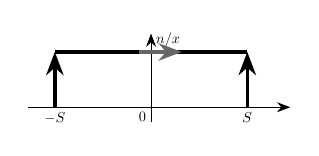
\begin{tikzpicture}[baseline=(current bounding box.center),scale=0.52,transform shape,>=Stealth] \draw[->] (-3.0,0) -- (3.4,0); \draw[->] (0,-0.35) -- (0,1.8); \node[below] at (-2.35,0) {$-S$}; \node[below] at (2.35,0) {$S$}; \node[below left] at (0,0) {$0$}; \node[above right] at (0,1.35) {$n/x$}; \draw[black,very thick,->] (-2.35,0) -- (-2.35,1.35); \draw[black,very thick,->] (2.35,0) -- (2.35,1.35); \draw[black,very thick] (-2.35,1.35) -- (2.35,1.35); \draw[black!60,very thick,->] (-0.3,1.35) -- (0.75,1.35); \end{tikzpicture}\)
	在两个竖直边上的积分满足估计
	\(\textstyle i\int_0^{n/x}e^{-\pi x(-S+\allowbreak{}i\eta)^2}\,d\eta +\allowbreak{} i\int_{n/x}^{0}e^{-\pi x(S+\allowbreak{}i\eta)^2}\,d\eta \ll\allowbreak{} \frac{n}{x}e^{-\pi xS^2+\allowbreak{}\pi n^2/x} \longrightarrow0 \qquad (S\to\allowbreak{}\infty).\)
	于是令 $S\to\infty$，得到
	\(\textstyle \int_{\mathbb R+\allowbreak{}in/x}e^{-\pi xz^2}\,dz =\allowbreak{} \int_{\mathbb R}e^{-\pi x\xi^2}\,d\xi =\allowbreak{} \frac{1}{\sqrt{x}}.\)
	因此
	\(\textstyle \widehat f(n)=\allowbreak{}\frac{1}{\sqrt{x}}e^{-\pi n^2/x}.\)
	代入 Poisson 求和公式，即得
	\(\textstyle \theta(x)=\allowbreak{}\frac{1}{\sqrt{x}}\theta\left(\frac1x\right).\)
\end{proof}

\weekmarker{第 12 周}

\begin{proof}[Theorem 8.1 的证明]
	先设 $\Re(s)>1$。由 Gamma 函数的积分公式，
	\(\textstyle \pi^{-s/2}\Gamma\left(\frac{s}{2}\right)\zeta(s) =\allowbreak{} \int_0^\infty \sum_{n=\allowbreak{}1}^{\infty}e^{-\pi n^2\xi} \xi^{s/2}\frac{d\xi}{\xi}\) \(\textstyle =\allowbreak{} \int_0^\infty \frac{\theta(\xi)-1}{2} \xi^{s/2}\frac{d\xi}{\xi}.\)
	这里可以交换求和与积分的次序，因为当 $\xi>0$ 时 $\theta(\xi)$ 绝对收敛。
	注意右端积分只有在 $\Re(s)>1$ 时收敛。事实上，当 $\xi$ 很小时，比如
	$0<\xi<1$，有
	\(\textstyle \theta(\xi)-1\ll\allowbreak{} \xi^{-1/2},\allowbreak{}\)
	而
	\(\textstyle \int_0^1 \xi^{-1/2}\xi^{s/2}\frac{d\xi}{\xi}\)
	只在 $\Re(s)>1$ 时收敛。

	现在把积分拆成两段：
	\(\textstyle \int_0^\infty \frac{\theta(\xi)-1}{2} \xi^{s/2}\frac{d\xi}{\xi} =\allowbreak{} \int_0^1 \frac{\theta(\xi)-1}{2} \xi^{s/2}\frac{d\xi}{\xi} +\allowbreak{} \int_1^\infty \frac{\theta(\xi)-1}{2} \xi^{s/2}\frac{d\xi}{\xi}.\)
	由 Lemma 8.3，第一项可以写成
	\(\textstyle \int_0^1 \frac{\theta(\xi)-1}{2} \xi^{s/2}\frac{d\xi}{\xi} =\allowbreak{} \frac12 \int_0^1 \left(\xi^{-1/2}\theta\left(\frac1\xi\right)-1\right) \xi^{s/2}\frac{d\xi}{\xi}\) \(\textstyle =\allowbreak{} \frac12 \int_0^1 \xi^{-1/2} \left(\theta\left(\frac1\xi\right)-1\right) \xi^{s/2}\frac{d\xi}{\xi}\) \(\textstyle \qquad +\allowbreak{} \frac12 \int_0^1 (\xi^{-1/2}-1)\xi^{s/2}\frac{d\xi}{\xi}.\)
	在第一项中作变量代换 $u=1/\xi$，得到
	\(\textstyle \frac12 \int_0^1 \xi^{-1/2} \left(\theta\left(\frac1\xi\right)-1\right) \xi^{s/2}\frac{d\xi}{\xi} =\allowbreak{} \frac12 \int_1^\infty (\theta(u)-1)u^{(1-s)/2}\frac{du}{u}.\)
	另一方面，
	\(\textstyle \frac12 \int_0^1 (\xi^{-1/2}-1)\xi^{s/2}\frac{d\xi}{\xi} =\allowbreak{} \frac{1}{s-1}-\frac1s =\allowbreak{} -\frac1s-\frac{1}{1-s}.\)
	总之得到
	\(\textstyle \pi^{-s/2}\Gamma\left(\frac{s}{2}\right)\zeta(s) =\allowbreak{} -\frac1s-\frac{1}{1-s}\) \(\textstyle \qquad +\allowbreak{} \int_1^\infty \frac{\theta(\xi)-1}{2} \left(\xi^{s/2}+\allowbreak{}\xi^{(1-s)/2}\right) \frac{d\xi}{\xi}. \quad\textup{(8.2)}\)
	这里注意，右端的积分对所有 $s\in\mathbb C$ 都收敛。因此右端定义了一个亚纯函数，从而给出了 $\zeta(s)$ 到整个复平面的亚纯延拓。并且，式 (8.2) 在把 $s$ 替换成 $1-s$ 时保持不变，于是得到函数方程
	\(\textstyle \pi^{-s/2}\Gamma\left(\frac{s}{2}\right)\zeta(s) =\allowbreak{} \pi^{-(1-s)/2} \Gamma\left(\frac{1-s}{2}\right)\zeta(1-s).\)
	至于 $\zeta(s)$ 的极点，我们已经看出它在半平面 $\Re(s)>0$ 中的唯一极点是 $s=1$，而且这是一个单极点。再由函数方程以及 $\Gamma(s)$ 在 $s=0$ 有一个单极点这个事实，可以看出 $\zeta(s)$ 在 $\mathbb C$ 中除 $s=1$ 以外没有其他极点。
\end{proof}

\begin{remark}
	由 Gamma 函数的性质，函数方程也可以写成
	\(\textstyle \zeta(1-s)=\allowbreak{}\chi(s)\zeta(s),\allowbreak{} \qquad \chi(s)=\allowbreak{}2(2\pi)^{-s}\Gamma(s)\cos\frac{\pi s}{2},\allowbreak{}\)
	或者等价地写成
	\(\textstyle \zeta(s) =\allowbreak{} 2^s\pi^{s-1}\sin\frac{\pi s}{2}\Gamma(1-s)\zeta(1-s).\)
	由于 $\Gamma(s)$ 与 $\zeta(s)$ 在 $\Re(s)>1$ 时都不为零，上面的恒等式说明 $\zeta(s)$ 在 $\Re(s)<0$ 中的零点恰好是
	\(\textstyle s=\allowbreak{}-2,\allowbreak{}-4,\allowbreak{}-6,\allowbreak{}\ldots,\allowbreak{}\)
	这些称为平凡零点（trivial zeros）。所有其他零点都位于带状区域
	\(\textstyle 0\leq\allowbreak{} \Re(s)\leq\allowbreak{} 1,\allowbreak{}\)
	这个区域称为临界带（critical strip）。
\end{remark}

\section{一阶整函数}

本节的目标是把 $\zeta$-函数表达成由它的零点指标化的无穷乘积，这称为 Hadamard 分解（Hadamard factorization）。由于这种分解对一类更一般的全纯函数有效，我们先为一般全纯函数建立定理，然后再应用到特殊情形 $\zeta^*(s)$。

\subsection{复分析中的一个定理}

复分析中一个熟知的定理说，所有满足
\(\textstyle f(s)\ll\allowbreak{} |s|^\alpha\)
的整函数（entire function）其实都是多项式，而且次数至多为 $\alpha$。下面的引理给出我们需要的形式。

\begin{lemma}[原文 Lemma 9.1]
	设 $C,\alpha>0$ 为实常数。如果 $g$ 是一个整函数，并且对所有 $s\in\mathbb C$ 满足
	\(\textstyle \Re g(s)\leq\allowbreak{} C(1+\allowbreak{}|s|^\alpha),\allowbreak{} \quad\textup{(9.1)}\)
	那么 $g$ 是次数至多为 $\alpha$ 的多项式。
\end{lemma}

\begin{proof}
	不妨假设 $g$ 在 $s=0$ 消失，否则把 $g(s)$ 换成 $g(s)-g(0)$。把 $g$ 写成 Taylor 级数
	\(\textstyle g(s)=\allowbreak{}\sum_{n=\allowbreak{}1}^{\infty}(a_n+\allowbreak{}ib_n)s^n,\allowbreak{}\)
	其中 $a_n,b_n\in\mathbb R$。这个级数在整个复平面上收敛。使用极坐标
	$s=re^{2\pi i\theta}$，则实部有展开
	\(\textstyle \Re g(re^{2\pi i\theta}) =\allowbreak{} \sum_{n=\allowbreak{}1}^{\infty}a_n\cos(2\pi n\theta)r^n - \sum_{n=\allowbreak{}1}^{\infty}b_n\sin(2\pi n\theta)r^n.\)
	回忆正交关系
	\(\textstyle \int_0^1 \cos(2\pi n\theta)\cos(2\pi \ell\theta)\,d\theta = \begin{cases} \frac12, & n=\ell\neq0,\\ 0, & n\neq \ell,\\ 1, & n=\ell=0, \end{cases}\)
	以及相应的正弦正交关系。将上式乘以 $\cos(2\pi \ell\theta)$ 并在 $\theta\in[0,1]$ 上积分，可得
	\(\textstyle a_\ell r^\ell =\allowbreak{} 2\int_0^1 \Re g(re^{2\pi i\theta})\cos(2\pi\ell\theta)\,d\theta.\)
	这里还用到 $g(0)=0$ 以及实部的平均值性质：
	\(\textstyle \int_0^1 \Re g(re^{2\pi i\theta})\,d\theta=\allowbreak{}\Re g(0)=\allowbreak{}0.\)
	因此由上界 (9.1)，
	\(\textstyle \int_0^1 |\Re g(re^{2\pi i\theta})|\,d\theta =\allowbreak{} 2\int_0^1 \max\{0,\allowbreak{}\Re g(re^{2\pi i\theta})\}\,d\theta \ll\allowbreak{} 1+\allowbreak{}r^\alpha.\)
	于是
	\(\textstyle |a_\ell| \leq\allowbreak{} \frac{2}{r^\ell} \int_0^1 |\Re g(re^{2\pi i\theta})|\,d\theta \ll\allowbreak{} r^{\alpha-\ell}.\)
	令 $r\to\infty$，当 $\ell>\alpha$ 时得到 $a_\ell=0$。同样地，乘以 $\sin(2\pi\ell\theta)$ 并积分，可以得到 $b_\ell=0$。因此当 $\ell>\alpha$ 时所有系数都为零，故 $g$ 是次数至多为 $\alpha$ 的多项式。
\end{proof}

\begin{definition}[有限阶函数]
	设 $f:\mathbb C\to\mathbb C$ 为整函数。如果存在常数 $\alpha>0$，使得对所有 $s\in\mathbb C$ 都有
	\(\textstyle f(s)=\allowbreak{}O\left(\exp(|s|^\alpha)\right),\allowbreak{}\)
	则称 $f$ 是有限阶（finite order）的。
\end{definition}

\begin{definition}[阶]
	如果整函数 $f$ 是有限阶的，则数
	\(\textstyle \inf\left\{ \alpha>0: f(s)\ll\allowbreak{} \exp(|s|^\alpha) \right\}\)
	称为 $f$ 的阶（order）。
\end{definition}

如果一个有限阶函数在 $\mathbb C$ 上没有零点，那么它有非常特殊的形式。

\begin{lemma}[原文 Lemma 9.2]
	设 $f$ 是有限阶整函数，并且在 $\mathbb C$ 上处处不为零。那么
	\(\textstyle f(s)=\allowbreak{}\exp(g(s)),\allowbreak{}\)
	其中 $g$ 是一个多项式。更精确地，$g$ 的次数至多为 $f$ 的阶。
\end{lemma}

\begin{proof}
	因为 $f$ 在 $\mathbb C$ 上没有零点，所以可以选取一个全纯的 $\log f(s)$。设
	\(\textstyle g(s)=\allowbreak{}\log f(s).\)
	若 $f$ 的阶为 $\alpha$，则对任意 $\varepsilon>0$，
	\(\textstyle \Re g(s)=\allowbreak{}\log |f(s)|\ll\allowbreak{} |s|^{\alpha+\allowbreak{}\varepsilon}.\)
	由 Lemma 9.1 的证明同样可以推出 $g$ 是多项式；令 $\varepsilon\to0$，可知 $g$ 的次数至多为 $\alpha$。
\end{proof}

现在我们需要研究带有零点的有限阶函数。下面的定理给出阶与零点分布之间的关系。

\begin{theorem}[Jensen 公式；原文 Theorem 9.3]
	设 $R>0$。设 $f$ 在圆盘
	\(\textstyle |s|\leq\allowbreak{} R\)
	的某个邻域中全纯，并且 $f$ 在 $s=0$ 处不为零，在圆周 $|s|=R$ 上也不为零。那么
	\(\textstyle \frac{1}{2\pi} \int_0^{2\pi}\log |f(Re^{i\theta})|\,d\theta =\allowbreak{} \log |f(0)| +\allowbreak{} \sum_\rho \log\frac{R}{|\rho|},\allowbreak{}\)
	其中 $\rho$ 遍历 $f$ 在 $|\rho|<R$ 中的零点，并按重数计算。
\end{theorem}

\begin{proof}
	把 $f$ 分解为
	\(\textstyle f(s)=\allowbreak{}\widetilde f(s)\prod_\rho (s-\rho),\allowbreak{}\)
	其中 $\rho$ 遍历圆盘 $|s|<R$ 中的零点，并按重数计算；而 $\widetilde f$ 在 $|s|\leq R$ 上全纯且不为零。于是
	\(\textstyle \log |f(s)| =\allowbreak{} \log|\widetilde f(s)| +\allowbreak{} \sum_\rho \log|s-\rho|.\)
	因此只需处理下面两种情形。

	第一，如果 $f$ 在 $|s|\leq R$ 中没有零点，那么 $\log f(s)$ 是全纯函数。由 Cauchy 公式，
	\(\textstyle \log |f(0)| =\allowbreak{} \Re \log f(0) =\allowbreak{} \frac{1}{2\pi}\int_0^{2\pi} \Re \log f(Re^{i\theta})\,d\theta =\allowbreak{} \frac{1}{2\pi}\int_0^{2\pi} \log |f(Re^{i\theta})|\,d\theta.\)

	第二，考虑 $f(s)=s-\xi$，其中 $|\xi|<R$。写
	\(\textstyle f(s)=\allowbreak{}f_1(s)f_2(s),\allowbreak{} \qquad f_1(s)=\allowbreak{}\frac{s-\xi}{R^2-\overline{\xi}s},\allowbreak{} \qquad f_2(s)=\allowbreak{}R^2-\overline{\xi}s.\)
	当 $|s|=R$ 时，
	\(\textstyle |f_1(s)|=\allowbreak{}\frac1R.\)
	另一方面，$f_2$ 在圆盘中没有零点，所以由第一种情形，
	\(\textstyle \frac{1}{2\pi}\int_0^{2\pi} \log |f_2(Re^{i\theta})|\,d\theta =\allowbreak{} \log |f_2(0)| =\allowbreak{} \log R^2.\)
	合并起来得到
	\(\textstyle \frac{1}{2\pi}\int_0^{2\pi} \log |Re^{i\theta}-\xi|\,d\theta =\allowbreak{} -\log R+\allowbreak{}\log R^2 =\allowbreak{} \log R.\)
	把这两个情形代回上面的分解，即得 Jensen 公式。
\end{proof}

作为 Jensen 公式的推论，我们有下面的零点计数估计。

\begin{theorem}[原文 Theorem 9.4]
	设 $\alpha>0$，并设 $f$ 是阶为 $\alpha$ 的整函数。那么对所有 $R\geq1$ 以及任意 $\varepsilon>0$，有
	\(\textstyle \sum_{|\rho|\leq\allowbreak{} R}1 \ll\allowbreak{} R^{\alpha+\allowbreak{}\varepsilon},\allowbreak{}\)
	其中 $\rho$ 遍历 $f$ 在 $|z|<R$ 中的零点，并按重数计算。
\end{theorem}

\begin{proof}
	不妨假设 $f(0)\neq0$；如果不是这样，则把 $f(s)$ 换成 $f(s)s^{-m}$，其中 $m$ 是合适的整数。也可以假设 $f$ 在圆周 $|s|=3R$ 上没有零点；否则把 $R$ 换成 $R+\delta$，其中某个实数 $\delta\in(0,1)$ 可以避开零点。

	由 Theorem 9.3，并使用 $f$ 的阶为 $\alpha$，得到
	\(\textstyle \sum_{|\rho|\leq\allowbreak{} R}1 \leq\allowbreak{} \sum_{|\rho|\leq\allowbreak{} R}\log\frac{3R}{|\rho|}\) \(\textstyle \leq\allowbreak{} \sum_{|\rho|\leq\allowbreak{} 3R}\log\frac{3R}{|\rho|}\) \(\textstyle =\allowbreak{} -\log|f(0)| +\allowbreak{} \frac{1}{2\pi} \int_0^{2\pi} \log|f(3Re^{i\theta})|\,d\theta \ll\allowbreak{} R^{\alpha+\allowbreak{}\varepsilon}.\)
	这就证明了定理。
\end{proof}

\begin{remark}
	作为这个定理的一个推论，如果 $f$ 的阶为 $\alpha$，那么对任何 $\varepsilon>0$，
	\(\textstyle \sum_\rho \frac{1}{|\rho|^{\alpha+\allowbreak{}\varepsilon}}<\infty,\allowbreak{}\)
	其中 $\rho$ 遍历 $f$ 的所有非零零点，并按重数计算。证明作为练习。
\end{remark}

现在我们准备证明本节的主要定理。

\begin{theorem}[Hadamard 分解；原文 Theorem 9.5]
	设 $f$ 是阶至多为 $1$ 的整函数。设 $k\geq0$ 为 $f$ 在 $s=0$ 处零点的阶数。那么存在常数 $A,B\in\mathbb C$，使得
	\(\textstyle f(s) =\allowbreak{} e^{A+\allowbreak{}Bs}s^k \prod_\rho \left(1-\frac{s}{\rho}\right)e^{s/\rho},\allowbreak{}\)
	其中 $\rho$ 遍历 $f$ 的所有非零零点，并按重数计算；乘积在不含零点的有界区域上一致收敛。
\end{theorem}

\begin{proof}
	先说明乘积的收敛性。设 $K\subset\mathbb C$ 为紧集。$K$ 中的零点只有有限多个。对于 $s\in K$，并且对 $K$ 外的零点 $\rho$，有
	\(\textstyle \left(1-\frac{s}{\rho}\right)e^{s/\rho} =\allowbreak{} 1+\allowbreak{}O_K\left(\frac{1}{|\rho|^2}\right).\)
	回忆：如果 $\sum a_n$ 绝对收敛，那么 $\prod(1+a_n)$ 收敛。由于 $f$ 的阶至多为 $1$，Theorem 9.4 推出
	\(\textstyle \sum_\rho\frac1{|\rho|^2}<\infty.\)
	于是乘积
	\(\textstyle P(s):=\allowbreak{} \prod_\rho \left(1-\frac{s}{\rho}\right)e^{s/\rho}\)
	在有界区域上一致收敛，并定义一个整函数。并且 $P$ 的零点恰好就是 $f$ 的非零零点，重数也相同。

	因此，在先把 $s=0$ 处的零点因子 $s^k$ 分离出来以后，商
	\(\textstyle \frac{f(s)}{s^kP(s)}\)
	是一个整函数，并且在 $\mathbb C$ 上处处不为零。下面证明这个商的阶至多为 $1$。由 Lemma 9.2，这将给出定理。

	因为 $f$ 本身按假设是阶至多为 $1$ 的，我们已经有 $f(s)$ 的上界。因此只需要给出 $P(s)$ 的下界。由于
	\(\textstyle \sum_\rho\frac1{|\rho|^2}<\infty,\allowbreak{}\)
	所有区间
	\(\textstyle \left(|\rho|-\frac1{|\rho|^2},\allowbreak{}\,|\rho|+\allowbreak{}\frac1{|\rho|^2}\right)\)
	的总长度是有限的。因此存在任意大的实数 $R$，使得
	\(\textstyle \bigl|R-|\rho|\bigr|>\frac1{|\rho|^2} \qquad \text{对所有零点 }\rho. \quad\textup{(9.2)}\)
	下面估计 $P(s)$ 在圆周 $|s|=R$ 上的大小。写
	\(\textstyle P(s)=\allowbreak{}P_1(s)P_2(s)P_3(s),\allowbreak{}\)
	其中
	\(\textstyle P_1(s)=\allowbreak{} \prod_{|\rho|\leq\allowbreak{} R/2} \left(1-\frac{s}{\rho}\right)e^{s/\rho},\allowbreak{}\)
	\(\textstyle P_2(s)=\allowbreak{} \prod_{R/2<|\rho|\leq\allowbreak{} 2R} \left(1-\frac{s}{\rho}\right)e^{s/\rho},\allowbreak{}\)
	以及
	\(\textstyle P_3(s)=\allowbreak{} \prod_{|\rho|>2R} \left(1-\frac{s}{\rho}\right)e^{s/\rho}.\)

	先估计 $P_1(s)$。对于满足 $|\rho|\leq R/2$ 的零点 $\rho$，有
	\(\textstyle \left| \left(1-\frac{s}{\rho}\right)e^{s/\rho} \right| \geq\allowbreak{} \left(\frac{|s|}{|\rho|}-1\right)e^{-|s|/|\rho|} > \exp\left(-\frac{R}{|\rho|}\right),\allowbreak{}\)
	当 $R$ 充分大时成立。因此
	\(\textstyle |P_1(s)| > \exp\left( -\sum_{|\rho|\leq\allowbreak{} R/2}\frac{R}{|\rho|} \right).\)
	又因为
	\(\textstyle \sum_{|\rho|\leq\allowbreak{} R/2}\frac1{|\rho|} \leq\allowbreak{} \left(\frac{R}{2}\right)^\varepsilon \sum_\rho \frac1{|\rho|^{1+\allowbreak{}\varepsilon}},\allowbreak{}\)
	所以
	\(\textstyle |P_1(s)|>\exp(-R^{1+\allowbreak{}\varepsilon}).\)

	再估计 $P_2(s)$。对于满足 $R/2<|\rho|\leq2R$ 的零点，由 (9.2) 可得
	\(\textstyle \left| \left(1-\frac{s}{\rho}\right)e^{s/\rho} \right| \geq\allowbreak{} e^{-2}\left|1-\frac{s}{\rho}\right|\) \(\textstyle \geq\allowbreak{} e^{-2}\frac{\bigl||s|-|\rho|\bigr|}{|\rho|} \geq\allowbreak{} e^{-2}\frac{\bigl|R-|\rho|\bigr|}{2R} \geq\allowbreak{} \frac{c}{R^3}\)
	其中 $c>0$ 为某个常数。由 Theorem 9.4，在区域 $R/2<|\rho|\leq2R$ 中至多有 $O(R^{1+\varepsilon})$ 个零点。因此
	\(\textstyle |P_2(s)| \geq\allowbreak{} (cR^{-3})^{CR^{1+\allowbreak{}\varepsilon}} > \exp(-R^{1+\allowbreak{}2\varepsilon})\)
	当 $R$ 充分大时成立。

	最后估计 $P_3(s)$。如果 $|\rho|>2R$，则 $|s/\rho|<1/2$。利用不等式
	\(\textstyle \left|\left(1-\frac{s}{\rho}\right)e^{s/\rho}\right| > \exp\left(-c\left|\frac{s}{\rho}\right|^2\right),\allowbreak{} \qquad |s/\rho|<\frac12,\allowbreak{}\)
	其中 $c$ 取充分小的常数，于是
	\(\textstyle |P_3(s)| > \exp\left( -cR^2\sum_{|\rho|>2R}\frac1{|\rho|^2} \right).\)
	注意到
	\(\textstyle \sum_{|\rho|>2R}\frac1{|\rho|^2} \leq\allowbreak{} (2R)^{-1+\allowbreak{}\varepsilon} \sum_\rho\frac1{|\rho|^{1+\allowbreak{}\varepsilon}},\allowbreak{}\)
	所以
	\(\textstyle |P_3(s)| > \exp(-R^{1+\allowbreak{}2\varepsilon})\)
	当 $R$ 充分大时成立。

	把 $P_1,P_2,P_3$ 的下界相乘，得到
	\(\textstyle |P(s)|>\exp(-3R^{1+\allowbreak{}2\varepsilon}) > \exp(-R^{1+\allowbreak{}3\varepsilon}) \qquad (|s|=\allowbreak{}R),\allowbreak{}\)
	其中 $R$ 充分大并满足 (9.2)。另一方面，由于 $f$ 的阶至多为 $1$，有
	\(\textstyle f(s)\ll\allowbreak{} \exp(R^{1+\allowbreak{}\varepsilon}) \qquad (|s|=\allowbreak{}R).\)
	于是
	\(\textstyle \frac{f(s)}{s^kP(s)} \ll\allowbreak{} \exp(R^{1+\allowbreak{}4\varepsilon}) \qquad (|s|=\allowbreak{}R). \quad\textup{(9.3)}\)
	最后，由于 $\sum_\rho 1/|\rho|^2$ 收敛，可以选取一列实数 $\{R_j\}_{j=1}^{\infty}$，使得
	\(\textstyle \lim_{j\to\allowbreak{}\infty}R_j=\allowbreak{}\infty,\allowbreak{} \qquad |R_{j+\allowbreak{}1}-R_j|\leq1,\allowbreak{}\)
	并且每个 $R_j$ 都满足 (9.2)。把 (9.3) 用在 $|s|=R_j$ 上，再用最大模原理，得到
	\(\textstyle \frac{f(s)}{s^kP(s)} \ll\allowbreak{} \exp\left((|s|+\allowbreak{}1)^{1+\allowbreak{}4\varepsilon}\right) \ll\allowbreak{} \exp(|s|^{1+\allowbreak{}5\varepsilon}).\)
	这说明 $f/(s^kP)$ 的阶至多为 $1$。由 Lemma 9.2，
	\(\textstyle \frac{f(s)}{s^kP(s)}=\allowbreak{}e^{A+\allowbreak{}Bs}\)
	对某些常数 $A,B\in\mathbb C$ 成立。代回 $P(s)$ 的定义，即得所需分解。
\end{proof}

\begin{remark}
	如果 $f$ 是阶为 $1$ 的整函数，那么
	\(\textstyle \sum_\rho \frac1{|\rho|}\)
	可能收敛，也可能不收敛。在收敛的情形中，可以得到没有 $1+\varepsilon$ 出现在指数里的估计，即
	\(\textstyle f(s)\ll\allowbreak{} e^{c|s|}\)
	对某个常数 $c>0$ 成立。
\end{remark}

\begin{proof}
	由 Hadamard 分解，
	\(\textstyle f(s)=\allowbreak{}s^k e^{A+\allowbreak{}Bs} \prod_\rho \left(1-\frac{s}{\rho}\right)e^{s/\rho}.\)
	若 $\sum_\rho 1/|\rho|<\infty$，则
	\(\textstyle |f(s)| \ll\allowbreak{} |s|^k e^{|B||s|} \prod_\rho \left(1+\allowbreak{}\frac{|s|}{|\rho|}\right)e^{|s|/|\rho|}\) \(\textstyle \ll\allowbreak{} e^{|s|}e^{|B||s|} \prod_\rho e^{2|s|/|\rho|} \ll\allowbreak{} e^{c|s|},\allowbreak{}\)
	其中
	\(\textstyle c=\allowbreak{}1+\allowbreak{}|B|+\allowbreak{}2\sum_\rho\frac1{|\rho|}\)
	是某个常数。
\end{proof}

\weekmarker{第 13 周}

下面记录两个 Hadamard 分解的例子。

\begin{example}[Hadamard 分解的例子]
	\(\textstyle \frac{1}{\Gamma(s)} =\allowbreak{} se^{\gamma s} \prod_{\ell=\allowbreak{}1}^{\infty} \left(1+\allowbreak{}\frac{s}{\ell}\right)e^{-s/\ell}.\)
	另外，
	\(\textstyle \sin \pi s =\allowbreak{} se^{A+\allowbreak{}Bs} \prod_{n=\allowbreak{}1}^{\infty}\left(1-\frac{s^2}{n^2}\right).\)
	回忆我们曾经用这个公式推出
	\(\textstyle \frac{\sin \pi s}{\pi s} =\allowbreak{} \prod_{n\geq\allowbreak{} 1}\left(1-\frac{s^2}{n^2}\right),\allowbreak{}\)
	从而证明反射公式
	\(\textstyle \Gamma(s)\Gamma(1-s)=\allowbreak{}\frac{\pi}{\sin \pi s}.\)
\end{example}

\subsection{\texorpdfstring{\(\zeta^*(s)\) 的 Hadamard 分解}{zeta*(s) 的 Hadamard 分解}}

现在把 Hadamard 分解，即 Theorem 9.5，应用到
$f(s)=\zeta^*(s)$，也就是整化的 Riemann $\zeta$-函数。

\begin{theorem}[原文 Theorem 9.6；\texorpdfstring{\(\zeta^*(s)\)}{zeta*(s)} 的 Hadamard 分解]
	$\zeta^*(s)$ 是一个阶为 $1$ 的整函数，并且满足
	\(\textstyle \zeta^*(s) =\allowbreak{} e^{Bs}\prod_\rho \left(1-\frac{s}{\rho}\right)e^{s/\rho},\allowbreak{}\)
		其中 $B$ 是一个复常数，乘积遍历 $\zeta^*(s)$ 的零点；也就是说，
		$\rho$ 遍历 $\zeta(s)$ 的非平凡零点，并按重数计算。
\end{theorem}

\begin{proof}
	由于 $\zeta^*(s)$ 已经是整函数，为了应用 Theorem 9.5，我们只需要验证它的阶为 $1$。
	借助函数方程
	\(\textstyle \zeta^*(s)=\allowbreak{}\zeta^*(1-s),\allowbreak{}\)
	只需在半平面 $\Re(s)\geq 1/2$ 中估计 $\zeta^*(s)$。
	由 Stirling 公式，
	\(\textstyle \log\Gamma(s) =\allowbreak{} \left(s-\frac12\right)\log s-s+\allowbreak{}\frac{\log 2\pi}{2} +\allowbreak{}O_\delta\left(\frac1{|s|}\right),\allowbreak{}\)
	从而
	\(\textstyle \log|\Gamma(s)| =\allowbreak{} \Re\log\Gamma(s) \leq\allowbreak{} |s|\log |s|.\)
	特别地，
	\(\textstyle \Gamma\left(\frac{s}{2}\right)\ll\allowbreak{} e^{|s|\log |s|}.\)
	另一方面，对 $\zeta(s)$，由前面得到的表达式
	\(\textstyle \zeta(s) =\allowbreak{} \frac{1}{s-1} +\allowbreak{}1 -s\int_1^\infty \frac{\rho(\xi)}{\xi^{s+\allowbreak{}1}}\,d\xi\)
	可知
	\(\textstyle \zeta(s)\ll\allowbreak{} |s| \qquad (|s|\to\allowbreak{}\infty)\)
	在这里所需的区域内成立。因此
	\(\textstyle \zeta^*(s) =\allowbreak{} s(s-1)\pi^{-s/2}\Gamma\left(\frac{s}{2}\right)\zeta(s) \ll\allowbreak{} e^{2|s|\log |s|}.\)
	这说明 $\zeta^*(s)$ 的阶至多为 $1$。

	反过来，令 $s\to\infty$ 沿实数趋于无穷。由
	\(\textstyle \Gamma(s)\sim\allowbreak{} e^{s\log s}\)
	可得，对实数 $s$，
	\(\textstyle \zeta^*(s)\gg\allowbreak{} e^{|s/2|\log |s/2|}.\)
	所以 $\zeta^*(s)$ 的阶至少为 $1$。于是 $\zeta^*(s)$ 的阶恰好为 $1$。

	由 Hadamard 分解（Theorem 9.5），
	\(\textstyle \zeta^*(s) =\allowbreak{} e^{A+\allowbreak{}Bs}\prod_\rho \left(1-\frac{s}{\rho}\right)e^{s/\rho}.\)
	这里 $A=0$，因为
	\(\textstyle \zeta^*(0)=\allowbreak{}\zeta^*(1) =\allowbreak{} \lim_{s\to1}(s-1)\zeta(s) =\allowbreak{} 1.\)
	因此得到所需公式。
\end{proof}

\begin{remark}
	$\zeta^*(s)$ 的零点恰好就是 $\zeta(s)$ 的非平凡零点（non-trivial zeros）。
	因此，下文在 $\zeta^*(s)$ 或 $\zeta(s)$ 的零点公式中出现的 $\sum_\rho$ 或 $\prod_\rho$，
	除非另有说明，都表示 $\rho$ 遍历这些非平凡零点，并按重数计算；
	若求和号附带 $|\Im\rho|<T$ 等条件，则是在这些非平凡零点中再加该条件。
\end{remark}

\begin{remark}
	$\zeta(s)$ 的零点关于直线 $\Re(s)=1/2$ 和直线 $\Im(s)=0$ 对称。
	事实上，若 $\zeta(\rho)=0$，则
	\(\textstyle \zeta(\overline{\rho}) =\allowbreak{} \overline{\zeta(\rho)} =\allowbreak{} 0,\allowbreak{}\)
	而由函数方程可得相应的关于 $\Re(s)=1/2$ 的对称性。
\end{remark}

\begin{theorem}[原文 Theorem 9.7]
	$\zeta(s)$ 的非平凡零点集是无限的。更精确地说，
	\(\textstyle \sum_\rho \frac{1}{|\rho|^\sigma}\)
	在 $\sigma=1$ 时发散，而对所有 $\sigma>1$ 收敛。
\end{theorem}

\begin{proof}
	当 $\sigma=1+\varepsilon$ 时，收敛性由 $\zeta^*(s)$ 是阶为 $1$ 的整函数以及 Theorem 9.4 得到。
	而
	\(\textstyle \sum_\rho \frac1{|\rho|}\)
	的发散性则来自 Theorem 9.5 后面的备注。既然这个级数发散，$\zeta(s)$ 的非平凡零点必然有无穷多个。
\end{proof}

Theorem 9.7 还有下面的推论。由于若 $\rho$ 是 $\zeta(s)$ 的非平凡零点，则
$\overline{\rho}$ 也是 $\zeta(s)$ 的非平凡零点，并且
\(\textstyle 0\leq\allowbreak{} \frac1{\rho}+\allowbreak{}\frac1{\overline{\rho}} =\allowbreak{} \frac{2\Re(\rho)}{|\rho|^2} \leq\allowbreak{} \frac{2}{|\rho|^2},\allowbreak{}\)
所以
\(\textstyle \lim_{x\to\allowbreak{}\infty}\sum_{|\rho|\leq\allowbreak{} x}\frac1{\rho} =\allowbreak{} \sum_{\Im\rho>0}\left(\frac1{\rho}+\allowbreak{}\frac1{\overline{\rho}}\right)\)
是收敛的。因此
\(\textstyle \sum_\rho \frac1{\rho}<\infty.\)
这里记号 $\sum_\rho 1/\rho$ 指的是在 $\zeta(s)$ 的非平凡零点上按 $|\rho|$ 截断的极限
\(\textstyle \lim_{x\to\allowbreak{}\infty}\sum_{|\rho|\leq\allowbreak{} x}\frac1{\rho}.\)
但是要记住，这个和并不是绝对收敛的；如果改变求和顺序，值可能发生变化。

稍后我们会推出整化 $\zeta$-函数的对数导数关于零点的表达式。为此先证明下面的引理。

\begin{lemma}[原文 Lemma 9.8]
	存在 $K>0$，使得
	\(\textstyle \zeta(s)\ll\allowbreak{} |s|^K\)
	对区域 $\sigma\geq -5$ 且 $|t|\geq 1$ 中的所有 $s=\sigma+it$ 成立。
	例如 $K=5$ 可以取。
\end{lemma}

\begin{proof}
	当 $\sigma>1+\varepsilon$ 时，
	\(\textstyle \zeta(s)\ll\allowbreak{} 1.\)
	前面已经看到，在相应的右半平面中，
	\(\textstyle \zeta(s)\ll\allowbreak{} |s|.\)
	最后，对区域 $-5\leq \sigma\leq 1/2$，使用 $\zeta(s)$ 的函数方程以及 Stirling 公式
	\(\textstyle \Gamma(\sigma+\allowbreak{}it) =\allowbreak{} \sqrt{2\pi}|t|^{\sigma-1/2}e^{-\frac{\pi}{2}|t|} \left(1+\allowbreak{}O\left(\frac1{|t|}\right)\right),\allowbreak{}\)
	即可得到
	\(\textstyle \zeta(s)\ll\allowbreak{} |s|^K\)
	对某个 $K>0$ 成立。
\end{proof}

记
\(\textstyle N(T) :=\allowbreak{} \sum_{\rho,\allowbreak{} |\Im\rho|\leq\allowbreak{} T}1,\allowbreak{}\)
其中 $\rho$ 遍历 $\zeta(s)$ 的非平凡零点；也就是说，$N(T)$ 是
$\zeta(s)$ 的虚部绝对值不超过 $T$ 的非平凡零点个数。

\begin{lemma}[原文 Lemma 9.9]
	对所有 $T\geq 2$，有
	\(\textstyle N(T)-N(T-1)\ll\allowbreak{} \log T,\allowbreak{} \qquad N(T)\ll\allowbreak{} T\log T.\)
\end{lemma}

\begin{proof}
	令
	\(\textstyle \tau=\allowbreak{}2+\allowbreak{}iT,\allowbreak{}\)
	并选取 $r\in[3,4]$，使得
	\(\textstyle \zeta^*\left(\tau+\allowbreak{}re^{2\pi i\theta}\right)\neq\allowbreak{} 0 \qquad (\theta\in\mathbb R).\)
	把 Jensen 公式（Theorem 9.3）应用到函数
	\(\textstyle f(s)=\allowbreak{}\zeta^*(\tau+\allowbreak{}s),\allowbreak{}\)
	得到
	\(\textstyle \sum_{\rho,\allowbreak{}\ |\rho-\tau|\leq\allowbreak{} r} \log\frac{r}{|\rho-\tau|} =\allowbreak{} \frac1{2\pi} \int_0^{2\pi} \log|\zeta^*(\tau+\allowbreak{}re^{i\theta})|\,d\theta -\log|\zeta^*(\tau)|.\)
		这里的 $\rho$ 是 $\zeta^*(s)$ 的零点，也就是 $\zeta(s)$ 的非平凡零点。
		由 Lemma 9.8，右端满足
	\(\textstyle \ll\allowbreak{} \log T.\)
	对左端，每一项
	\(\textstyle \log\frac{r}{|\rho-\tau|}\)
		都是非负的。限制在满足 $\Im\rho\in[T-1,T]$ 的非平凡零点上，由于非平凡零点满足
	$0\leq\Re\rho\leq 1$，且 $\tau=2+iT$，这些零点都落在以 $\tau$ 为圆心、半径 $r$ 的圆盘中所需的矩形范围内：
	\(\textstyle 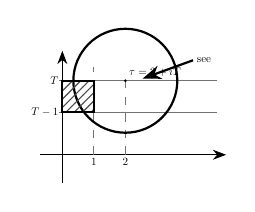
\begin{tikzpicture}[baseline=(current bounding box.center),scale=0.40,transform shape,>=Stealth] \draw[->] (-0.7,0) -- (5.2,0); \draw[->] (0,-0.9) -- (0,3.3); \node[left] at (0,2.35) {$T$}; \node[left] at (0,1.35) {$T-1$}; \draw[black!55] (-0.1,2.35) -- (4.9,2.35); \draw[black!55] (-0.1,1.35) -- (4.9,1.35); \draw[black!55,dashed] (1,0) -- (1,2.8); \draw[black!55,dashed] (2,0) -- (2,2.35); \node[below] at (1,0) {$1$}; \node[below] at (2,0) {$2$}; \coordinate (tau) at (2,2.35); \fill (tau) circle (1.4pt); \node[above right] at (tau) {$\tau=2+iT$}; \draw[thick] (tau) circle (1.65); \draw[black,pattern=north east lines,pattern color=black!70] (0,1.35) rectangle (1,2.35); \draw[black,thick] (0,1.35) rectangle (1,2.35); \draw[->,thick] (4.15,3.0) -- (2.55,2.42); \node[right] at (4.15,3.0) {see}; \end{tikzpicture}\)
	于是
	\(\textstyle \log\frac{3}{\sqrt5}\bigl(N(T)-N(T-1)\bigr) \leq\allowbreak{} \sum_{\rho,\allowbreak{} \Im\rho\in[T-1,\allowbreak{}T]} \log\frac{r}{|\rho-\tau|} \ll\allowbreak{} \log T.\)
	所以
	\(\textstyle N(T)-N(T-1)\ll\allowbreak{} \log T.\)
	进一步求和得
	\(\textstyle N(T)\ll\allowbreak{} T\log T.\)
\end{proof}

\chapter{素数定理}
\label{chap:prime-number-theorem}

现在我们有了证明素数定理（prime number theorem）的工具。目标是证明
\(\textstyle \psi(x) :=\allowbreak{} \sum_{n\leq\allowbreak{} x}\Lambda(n) =\allowbreak{} x+\allowbreak{}\text{``error term''}.\)
由于
\(\textstyle \sum_{n=\allowbreak{}1}^{\infty}\frac{\Lambda(n)}{n^s} =\allowbreak{} -\frac{\zeta'}{\zeta}(s),\allowbreak{}\)
想法是使用 Perron 公式（Perron's formula），把 $\psi(x)$ 写成形如
\(\textstyle \frac{1}{2\pi i} \int -\frac{\zeta'}{\zeta}(s)\frac{x^s}{s}\,ds\)
的复积分，然后把积分直线移动到 $\Re(s)=1$ 的左边。在这个过程中，$s=1$ 处的留数会给出 $\psi(x)$ 渐近公式中的主项；剩下需要说明的是余下积分相对于主项是低阶项。

\section{\texorpdfstring{\(\zeta'/\zeta(s)\)}{zeta'/zeta(s)} 的性质}

因为与 $\Lambda(n)$ 关联的 Dirichlet 级数是
\(\textstyle \sum_{n=\allowbreak{}1}^{\infty}\frac{\Lambda(n)}{n^s} =\allowbreak{} -\frac{\zeta'}{\zeta}(s),\allowbreak{}\)
我们需要理解 $\zeta'/\zeta(s)$ 的性质。

首先考虑半平面 $\Re(s)\geq 2$。有
\(\textstyle \left|\frac{\zeta'}{\zeta}(s)\right| \leq\allowbreak{} \sum_{n\geq1}\frac{\Lambda(n)}{n^\sigma} =\allowbreak{} -\frac{\zeta'}{\zeta}(\sigma).\)
由于
\(\textstyle -\frac{\zeta'}{\zeta}(\sigma) =\allowbreak{} \frac1{\sigma-1}+\allowbreak{}O(1),\allowbreak{}\)
所以当 $\Re(s)\geq 2$ 时，
\(\textstyle \frac{\zeta'}{\zeta}(s)\ll\allowbreak{} 1. \quad\textup{(10.1)}\)

其次考虑区域 $\Re(s)\leq -1$，并假设
\(\textstyle |s+\allowbreak{}2n|\geq\allowbreak{} \frac14 \qquad (n\in\mathbb N).\)
由函数方程
\(\textstyle \zeta(s) =\allowbreak{} 2^s\pi^{s-1}\sin\left(\frac{\pi s}{2}\right)\Gamma(1-s)\zeta(1-s),\allowbreak{}\)
等价地，
\(\textstyle \zeta(1-s) =\allowbreak{} 2^{-s}\pi^{-s}\cos\left(\frac{\pi s}{2}\right)\Gamma(s)\zeta(s).\)
取对数导数，得到
\(\textstyle -\frac{\zeta'}{\zeta}(1-s) =\allowbreak{} -\log 2\pi -\frac{\pi}{2}\tan\left(\frac{\pi s}{2}\right) +\allowbreak{}\frac{\Gamma'}{\Gamma}(s) +\allowbreak{}\frac{\zeta'}{\zeta}(s).\)
这里若 $s$ 远离相应的极点，例如满足上面的 $|s+2n|\geq 1/4$，则三角函数项有界。于是当 $\Re(s)\leq -1$ 且
$|s+2n|\geq 1/4$ 对所有 $n\in\mathbb N$ 成立时，
\(\textstyle \frac{\zeta'}{\zeta}(s)\ll\allowbreak{} \log |s|.\)

现在剩下要考虑的是带状区域
\(\textstyle -1\leq\allowbreak{} \Re(s)\leq\allowbreak{} 2.\)

\begin{lemma}[原文 Lemma 10.1]
	对所有 $s=\sigma+it\in\mathbb C$，若
	\(\textstyle -1\leq\allowbreak{} \sigma\leq\allowbreak{} 2,\allowbreak{} \qquad |t|\geq\allowbreak{} 2,\allowbreak{}\)
	则
	\(\textstyle \frac{\zeta'}{\zeta}(s) =\allowbreak{} \sum_{\rho,\allowbreak{} |\Im\rho-t|<1} \frac1{s-\rho} +\allowbreak{} O(\log |t|).\)
		其中 $\rho$ 遍历 $\zeta(s)$ 的非平凡零点。
	\end{lemma}

	\begin{proof}
		对
	\(\textstyle \zeta^*(s) =\allowbreak{} s(s-1)\pi^{-s/2}\Gamma\left(\frac{s}{2}\right)\zeta(s)\)
	以及 Hadamard 分解
	\(\textstyle \zeta^*(s) =\allowbreak{} e^{Bs}\prod_\rho \left(1-\frac{s}{\rho}\right)e^{s/\rho}\)
		其中 $\rho$ 遍历 $\zeta(s)$ 的非平凡零点。
			取对数导数，得到
	\(\textstyle \frac{(\zeta^*)'}{\zeta^*}(s) =\allowbreak{} \frac1s+\allowbreak{}\frac1{s-1} -\frac12\log\pi +\allowbreak{}\frac12\frac{\Gamma'}{\Gamma}\left(\frac{s}{2}\right) +\allowbreak{} \frac{\zeta'}{\zeta}(s),\allowbreak{}\)
	同时
	\(\textstyle \frac{(\zeta^*)'}{\zeta^*}(s) =\allowbreak{} B+\allowbreak{} \sum_\rho \left(\frac1{s-\rho}+\allowbreak{}\frac1{\rho}\right).\)
	因此
	\(\textstyle \frac{\zeta'}{\zeta}(s) =\allowbreak{} -\frac1s-\frac1{s-1} +\allowbreak{}\frac12\log\pi -\frac12\frac{\Gamma'}{\Gamma}\left(\frac{s}{2}\right) +\allowbreak{} \sum_\rho \left(\frac1{s-\rho}+\allowbreak{}\frac1{\rho}\right) +\allowbreak{} B.\)
	顺便记下，由 Gamma 函数的性质还可以进一步推出
	\(\textstyle \frac{\zeta'}{\zeta}(s) =\allowbreak{} -\frac1{s-1} +\allowbreak{} \sum_\rho \left(\frac1{s-\rho}+\allowbreak{}\frac1{\rho}\right) +\allowbreak{} \sum_{m=\allowbreak{}1}^{\infty} \left(\frac1{s+\allowbreak{}2m}-\frac1{2m}\right) +\allowbreak{} \frac{\log\pi}{2} +\allowbreak{} B.\)
	由 Stirling 公式可知
	\(\textstyle \frac{\Gamma'}{\Gamma}(s) =\allowbreak{} \log s+\allowbreak{}O_\varepsilon\left(\frac1{|s|}\right).\)
	所以当 $-1\leq\sigma\leq 2$ 且 $|t|\geq2$ 时，
	\(\textstyle \frac{\zeta'}{\zeta}(s) =\allowbreak{} \sum_\rho \left(\frac1{s-\rho}+\allowbreak{}\frac1{\rho}\right) +\allowbreak{} O(\log |t|). \quad\textup{(10.2)}\)
	把 $s=2+it$ 代入，得到
	\(\textstyle \frac{\zeta'}{\zeta}(2+\allowbreak{}it) =\allowbreak{} \sum_\rho \left(\frac1{2+\allowbreak{}it-\rho}+\allowbreak{}\frac1{\rho}\right) +\allowbreak{} O(\log |t|). \quad\textup{(10.3)}\)
	而由 (10.1)，左端是 $O(1)$。用 (10.2) 减去 (10.3)，得到
	\(\textstyle \frac{\zeta'}{\zeta}(s) =\allowbreak{} \sum_\rho \left( \frac1{s-\rho} - \frac1{2+\allowbreak{}it-\rho} \right) +\allowbreak{} O(\log |t|).\)

		先看满足 $|\Im\rho-t|\leq1$ 的非平凡零点。由 Lemma 9.9，
	\(\textstyle \sum_{|\Im\rho-t|\leq1}\frac1{|2+\allowbreak{}it-\rho|} \leq\allowbreak{} \sum_{|\Im\rho-t|\leq1}1 \ll\allowbreak{} \log |t|.\)
		接着考虑满足 $|\Im\rho-t|>1$ 的非平凡零点。此时
	\(\textstyle |s-\rho|\asymp\allowbreak{} |t-\Im\rho|.\)
	因此
	\(\textstyle \frac1{s-\rho} - \frac1{2+\allowbreak{}it-\rho} =\allowbreak{} \frac{2-\sigma}{(s-\rho)(2+\allowbreak{}it-\rho)} \ll\allowbreak{} \frac1{|t-\Im\rho|^2}.\)
	于是
	\(\textstyle \sum_{|\Im\rho-t|>1} \left( \frac1{s-\rho} - \frac1{2+\allowbreak{}it-\rho} \right)\) \(\textstyle \qquad\ll\allowbreak{} \sum_{n\geq1} \sum_{\rho,\allowbreak{} n\leq\allowbreak{} |\Im\rho-t|\leq\allowbreak{} n+\allowbreak{}1} \frac1{|t-\Im\rho|^2}\) \(\textstyle \qquad\ll\allowbreak{} \sum_{n\geq1}\frac{\log(|t|+\allowbreak{}n)}{n^2} \ll\allowbreak{} \sum_{n\geq1}\frac{\log |t|\log n}{n^2} \ll\allowbreak{} \log |t|.\)
	综上，
	\(\textstyle \frac{\zeta'}{\zeta}(s) =\allowbreak{} \sum_{\rho,\allowbreak{} |\Im\rho-t|<1} \frac1{s-\rho} +\allowbreak{} O(\log |t|).\)
\end{proof}

\section{显式公式}

回忆
\(\textstyle \psi(x)=\allowbreak{}\sum_{n\leq\allowbreak{} x}\Lambda(n).\)
由于 $\psi(x)$ 在素数幂处有不连续点，我们定义
\(\textstyle \psi_0(x) := \begin{cases} \psi(x), & x\notin\mathbb Z,\\ \psi(x)-\frac{\Lambda(x)}{2}, & x\in\mathbb Z. \end{cases}\)

\begin{theorem}[显式公式；原文 Theorem 10.2]
	对 $x>2$，有
	\(\textstyle \psi_0(x) =\allowbreak{} x - \sum_\rho \frac{x^\rho}{\rho} - \frac{\zeta'}{\zeta}(0) - \frac12\log(1-x^{-2}).\)
	其中 $\rho$ 遍历 $\zeta(s)$ 的非平凡零点。
\end{theorem}

这里
\(\textstyle -\frac12\log(1-x^{-2}) =\allowbreak{} \sum_{m=\allowbreak{}1}^{\infty}\frac{x^{-2m}}{2m}.\)
就像 Perron 公式一样，这个公式由下面的定理令 $T\to\infty$ 得到。

\begin{theorem}[有效显式公式；原文 Theorem 10.3]
	对 $x,T>2$，有
	\(\textstyle \psi_0(x) =\allowbreak{} x - \sum_{\rho,\allowbreak{} |\Im\rho|<T}\frac{x^\rho}{\rho} - \frac{\zeta'}{\zeta}(0) - \frac12\log(1-x^{-2}) +\allowbreak{} R(x,\allowbreak{}T),\allowbreak{} \quad\textup{(10.4)}\)
	这里 $\rho$ 遍历 $\zeta(s)$ 的非平凡零点，并且只取满足
	$|\Im\rho|<T$ 的那些零点；其中
	\(\textstyle R(x,\allowbreak{}T) \ll\allowbreak{} \frac{x}{T}(\log xT)^2 +\allowbreak{} \log x\min\left(1,\allowbreak{}\frac{x}{T\langle x\rangle}\right),\allowbreak{}\)
	并且
	\(\textstyle \langle x\rangle :=\allowbreak{} \min\{|x-p^\ell|:\ p\in\mathbb P,\allowbreak{}\ \ell\in\mathbb N,\allowbreak{}\ x\neq\allowbreak{} p^\ell\}.\)
\end{theorem}

\begin{proof}
	回忆 Perron 公式说：若
	\(\textstyle L_f(s)=\allowbreak{}\sum_{n=\allowbreak{}1}^{\infty}\frac{f(n)}{n^s}\)
	在 $s=c$ 处绝对收敛，则
	\(\textstyle \sum_{n\leq\allowbreak{} x}^{*}f(n) =\allowbreak{} \frac1{2\pi i} \int_{c-iT}^{c+\allowbreak{}iT} L_f(s)\frac{x^s}{s}\,ds +\allowbreak{} O\left( \sum_{n=\allowbreak{}1}^{\infty} \frac{x^c|f(n)|}{n^c(1+\allowbreak{}T|\log(x/n)|)} +\allowbreak{} \frac{c}{T}|f(x)| \right).\)
	这里星号表示：如果 $x\in\mathbb Z$，那么最后一项 $f(x)$ 要替换成 $f(x)/2$。

	把公式应用到 $f(n)=\Lambda(n)$，并取
	\(\textstyle c=\allowbreak{}1+\allowbreak{}\frac1{\log x},\allowbreak{}\)
	得到
	\(\textstyle \psi_0(x) =\allowbreak{} \frac1{2\pi i} \int_{c-iT}^{c+\allowbreak{}iT} -\frac{\zeta'}{\zeta}(s)\frac{x^s}{s}\,ds +\allowbreak{} O(\Sigma),\allowbreak{}\)
	其中
	\(\textstyle \Sigma =\allowbreak{} \sum_{n\geq\allowbreak{}1,\allowbreak{} n\neq\allowbreak{} x} \frac{x^c\Lambda(n)}{n^c(1+\allowbreak{}T|\log(x/n)|)} +\allowbreak{} \frac{c}{T}\Lambda(x).\)
	我们需要证明
	\(\textstyle \Sigma \ll\allowbreak{} \frac{x(\log x)^2}{T} +\allowbreak{} \log x\min\left(1,\allowbreak{}\frac{x}{T\langle x\rangle}\right). \quad\textup{(10.5)}\)
	此外还需要证明
	\(\textstyle \frac1{2\pi i} \int_{c-iT}^{c+\allowbreak{}iT} -\frac{\zeta'}{\zeta}(s)\frac{x^s}{s}\,ds\) \(\textstyle \qquad=\allowbreak{} x - \sum_{\rho,\allowbreak{} |\Im\rho|<T}\frac{x^\rho}{\rho} - \frac{\zeta'}{\zeta}(0) - \frac12\log(1-x^{-2}) +\allowbreak{} O\left(\frac{x(\log xT)^2}{T}\right). \quad\textup{(10.6)}\)

	先证明 (10.5)。把
	\(\textstyle \Sigma=\allowbreak{}\Sigma_1+\allowbreak{}\Sigma_2+\allowbreak{}\Sigma_3\)
	分成三段，其中 $\Sigma_1$ 对应 $n\leq x/2$，$\Sigma_2$ 对应
	$x/2<n<2x$ 且 $n\neq x$，$\Sigma_3$ 对应 $n\geq 2x$。

	在 $\Sigma_1$ 中有 $\log(x/n)\gg 1$，因此
	\(\textstyle \Sigma_1 \ll\allowbreak{} \frac{x}{T}\sum_{n\geq1}\frac{\Lambda(n)}{n^c} \ll\allowbreak{} \frac{x}{T}\left|\frac{\zeta'}{\zeta}(c)\right| \ll\allowbreak{} \frac{x\log x}{T}.\)
	这里用到了
	\(\textstyle x^c=\allowbreak{}x^{1+\allowbreak{}1/\log x}=\allowbreak{}ex,\allowbreak{} \qquad \frac{\zeta'}{\zeta}(c)\sim\allowbreak{} \frac{1}{c-1}=\allowbreak{}\log x.\)

	为了估计 $\Sigma_2$，令
	\(\textstyle x_0:=\allowbreak{}\max\{p^\ell:\ p\in\mathbb P,\allowbreak{}\ \ell\in\mathbb N,\allowbreak{}\ p^\ell<x\}.\)
	注意如果 $n>x_0$，那么在 $\Sigma_2$ 中有 $\Lambda(n)=0$。因此只需要考虑
	$x/2<n\leq x_0$。
	若 $x/2<n<x_0$，则
	\(\textstyle \log\frac{x}{n} \geq\allowbreak{} \log\frac{x_0}{n} =\allowbreak{} -\log\left(1-\frac{x_0-n}{x_0}\right) \geq\allowbreak{} \frac{x_0-n}{x_0}.\)
	于是
	\(\textstyle \sum_{x/2<n<x_0} \frac{x^c\Lambda(n)}{n^c(1+\allowbreak{}T|\log(x/n)|)} \ll\allowbreak{} \sum_{x/2<n<x_0} \frac{x\Lambda(n)}{n(1+\allowbreak{}T(x_0-n)/x_0)}\) \(\textstyle \ll\allowbreak{} \log x \sum_{x/2<n<x_0} \frac1{1+\allowbreak{}T(x_0-n)/x_0}.\)
	而 $n=x_0$ 的项满足
	\(\textstyle \frac{x^c\Lambda(x_0)}{x_0^c(1+\allowbreak{}T|\log(x/x_0)|)} \ll\allowbreak{} \min\left\{\Lambda(x_0),\allowbreak{}\frac{\Lambda(x_0)}{T|\log(x/x_0)|}\right\}\)
	并且
	\(\textstyle \ll\allowbreak{} \min\left\{ \log x,\allowbreak{} \frac{x\log x}{T\langle x\rangle} \right\}.\)
	合在一起得到
	\(\textstyle \Sigma_2 \ll\allowbreak{} \frac{x(\log x)^2}{T} +\allowbreak{} \min\left\{ \log x,\allowbreak{} \frac{x\log x}{T\langle x\rangle} \right\}.\)
	同样的估计也适用于 $\Sigma_3$。因此得到 (10.5)。

	接下来证明 (10.6)。回忆
	% 第 13 周原手稿此处的记号疑似写成整化 zeta 的对数导数；按前后文的积分核修正为 \zeta'/\zeta。
	\(\textstyle -\frac{\zeta'}{\zeta}(s) =\allowbreak{} \frac1{s-1} - \sum_\rho \left(\frac1{s-\rho}+\allowbreak{}\frac1{\rho}\right) - \sum_{m=\allowbreak{}1}^{\infty} \left(\frac1{s+\allowbreak{}2m}-\frac1{2m}\right) - \frac{\gamma}{2} - \frac{\log\pi}{2} - B.\)
	这里 $\rho$ 遍历 $\zeta(s)$ 的非平凡零点。特别地，如果
	$\rho$ 是 $\zeta(s)$ 的非平凡零点，则
	\(\textstyle \operatorname*{Res}_{s=\allowbreak{}\rho} \left( -\frac{\zeta'}{\zeta}(s)\frac{x^s}{s} \right) =\allowbreak{} -\frac{x^\rho}{\rho}.\)
	另外，
	\(\textstyle \operatorname*{Res}_{s=\allowbreak{}0} \left( -\frac{\zeta'}{\zeta}(s)\frac{x^s}{s} \right) =\allowbreak{} -\frac{\zeta'}{\zeta}(0),\allowbreak{}\)
	并且
	\(\textstyle \operatorname*{Res}_{s=\allowbreak{}1} \left( -\frac{\zeta'}{\zeta}(s)\frac{x^s}{s} \right) =\allowbreak{} x.\)

	不妨假设 $T$ 满足
	\(\textstyle T\neq\allowbreak{} \Im\rho\)
	对所有非平凡零点 $\rho$ 成立。令 $U\in\mathbb N$ 为奇整数。由 Cauchy 留数定理（Cauchy's residue theorem），有
	\(\textstyle \frac1{2\pi i} \int_{c-iT}^{c+\allowbreak{}iT} -\frac{\zeta'}{\zeta}(s)\frac{x^s}{s}\,ds\) \(\textstyle \qquad=\allowbreak{} x - \sum_{\rho,\allowbreak{} |\Im\rho|<T}\frac{x^\rho}{\rho} - \frac{\zeta'}{\zeta}(0) +\allowbreak{} \sum_{m<U/2}\frac{x^{-2m}}{2m} +\allowbreak{} I_1+\allowbreak{}I_2+\allowbreak{}I_3,\allowbreak{} \quad\textup{(10.7)}\)
	其中
	\(\textstyle I_j =\allowbreak{} \frac1{2\pi i} \int_{\gamma_j} -\frac{\zeta'}{\zeta}(s)\frac{x^s}{s}\,ds.\)
	这里 $\gamma_1$ 是从 $c-iT$ 到 $-U-iT$ 的线段，$\gamma_2$ 是从
	$-U-iT$ 到 $-U+iT$ 的线段，$\gamma_3$ 是从 $-U+iT$ 到 $c+iT$ 的线段。
	% compact: skipped contour figure in theorem 11.2.2 / explicit formula proof.

	先估计 $I_2$。由于在 $\Re(s)<-1$ 且 $|s+2n|\geq 1/4$ 时有
	\(\textstyle \frac{\zeta'}{\zeta}(s)\ll\allowbreak{} \log|s|,\allowbreak{}\)
	所以
	\(\textstyle I_2 \ll\allowbreak{} \int_{-T}^{T} \log(U+\allowbreak{}|t|)\frac{x^{-U}}{U}\,dt \ll\allowbreak{} \frac{T\log T\log U}{Ux^U} \longrightarrow\allowbreak{} 0 \qquad (U\to\allowbreak{}\infty).\)

	接着估计 $I_1+I_3$。由于区间 $[T-1,T+1]$ 中至多有 $O(\log T)$ 个非平凡零点 $\rho$，
	所以总可以选择
	\(\textstyle \widetilde T\in[T-1,\allowbreak{}T+\allowbreak{}1]\)
	使得
	\(\textstyle |\Im\rho-\widetilde T|\gg\allowbreak{} (\log T)^{-1}\)
	对所有非平凡零点 $\rho$ 成立。于是可以假设 (10.4) 中的参数 $T$ 满足
	\(\textstyle |\Im\rho-T|\gg\allowbreak{} \frac1{\log T} \qquad \text{对所有非平凡零点 }\rho\text{ 成立}. \quad\textup{(10.8)}\)
	因为把 $T$ 换成 $\widetilde T$ 引入的误差至多为
	\(\textstyle \sum_{\rho,\allowbreak{} T-1\leq\allowbreak{}|\Im\rho|\leq\allowbreak{} T+\allowbreak{}1} \frac{x^\rho}{\rho} \ll\allowbreak{} x \sum_{\rho,\allowbreak{} T-1\leq\allowbreak{}|\Im\rho|\leq\allowbreak{} T+\allowbreak{}1} \frac1{|\rho|} \ll\allowbreak{} \frac{x}{T}\log T,\allowbreak{}\)
	这可以吸收到 (10.4) 的误差项中。

	由 Lemma 10.1，对所有满足 $-1\leq\sigma\leq2$ 且 $|t|\geq2$ 的
	$s=\sigma+it$，有
	\(\textstyle \frac{\zeta'}{\zeta}(s) =\allowbreak{} \sum_{\rho,\allowbreak{} |\Im\rho-t|<1} \frac1{s-\rho} +\allowbreak{} O(\log |t|).\)
	再由 (10.8)，当 $s=\sigma+iT$ 且 $-1\leq\sigma\leq2$ 时，
	\(\textstyle \left|\frac{\zeta'}{\zeta}(s)\right| \ll\allowbreak{} \log T +\allowbreak{} \sum_{\rho,\allowbreak{} |\Im\rho-T|<1} \frac1{|s-\rho|} \ll\allowbreak{} (\log T)^2.\)
	因此
	\(\textstyle I_1+\allowbreak{}I_3 \ll\allowbreak{} \int_{-U}^{-1} \left|\frac{\zeta'}{\zeta}(s)\right| \left|\frac{x^s}{s}\right|\,d\sigma +\allowbreak{} \int_{-1}^{c} \left|\frac{\zeta'}{\zeta}(s)\right| \left|\frac{x^s}{s}\right|\,d\sigma.\)
	这里分别沿水平线 $\Im(s)=\pm T$ 积分。于是
	\(\textstyle I_1+\allowbreak{}I_3 \ll\allowbreak{} \int_{-U}^{-1} \log T\,\frac{x^\sigma}{T}\,d\sigma +\allowbreak{} \int_{-1}^{c} \frac{(\log T)^2x^\sigma}{T}\,d\sigma\) \(\textstyle \ll\allowbreak{} \frac{\log T}{T}\cdot\frac{1}{x\log x} +\allowbreak{} \frac{(\log T)^2}{T}\cdot\frac{x}{\log x}.\)
	把这些估计代入 (10.7)，得到
	\(\textstyle \frac1{2\pi i} \int_{c-iT}^{c+\allowbreak{}iT} -\frac{\zeta'}{\zeta}(s)\frac{x^s}{s}\,ds\) \(\textstyle \qquad=\allowbreak{} x - \sum_{\rho,\allowbreak{} |\Im\rho|<T}\frac{x^\rho}{\rho} - \frac{\zeta'}{\zeta}(0) +\allowbreak{} \sum_{m<U/2}\frac{x^{-2m}}{2m} +\allowbreak{} O\left( \frac{T\log T\log U}{Ux^U} +\allowbreak{} \frac{x(\log T)^2}{T\log x} \right).\)
	\weekmarker{第 14 周}

	注意，上面的误差项关于 $U$ 是一致的。令 $U\to\infty$，得到
	\(\textstyle \frac1{2\pi i} \int_{c-iT}^{c+\allowbreak{}iT} -\frac{\zeta'}{\zeta}(s)\frac{x^s}{s}\,ds\) \(\textstyle \qquad=\allowbreak{} x - \sum_{\rho,\allowbreak{} |\Im\rho|<T}\frac{x^\rho}{\rho} - \frac{\zeta'}{\zeta}(0) +\allowbreak{} \sum_{m=\allowbreak{}1}^{\infty}\frac{x^{-2m}}{2m} +\allowbreak{} O\left( \frac{x(\log T)^2}{T\log x} \right),\allowbreak{}\)
	这推出 (10.6)。结合 (10.5) 与 (10.6)，Theorem 10.3 得证。
\end{proof}

\section{\texorpdfstring{\(\zeta(s)\) 的无零区域}{zeta(s) 的无零区域}}

从显式公式（explicit formula），也就是 Theorem 10.3，推出 $\psi(x)$ 的渐近公式时，
必须知道 $\zeta(s)$ 的非平凡零点 $\rho$ 的位置。本节目标是在临界带（critical strip）
\(\textstyle 0\leq\allowbreak{} \Re(s)\leq\allowbreak{} 1\)
中找出一块 $\zeta(s)\neq 0$ 的区域。

我们需要用到下面的初等恒等式：
\(\textstyle 3+\allowbreak{}4\cos\alpha+\allowbreak{}\cos 2\alpha =\allowbreak{} 2(1+\allowbreak{}\cos\alpha)^2 \geq\allowbreak{} 0 \qquad (\alpha\in\mathbb R). \qquad\text{(10.9)}\)

\begin{theorem}[原文 Theorem 10.4]
	对所有 $t\in\mathbb R\setminus\{0\}$，有
	\(\textstyle \zeta(1+\allowbreak{}it)\neq\allowbreak{} 0.\)
\end{theorem}

\begin{proof}
	对 $\sigma=\Re(s)>1$，由 Euler 乘积（Euler product）可得
	\(\textstyle \zeta(s) =\allowbreak{} \prod_p (1-p^{-s})^{-1}.\)
	因此
	\(\textstyle \log\zeta(s) =\allowbreak{} \sum_p -\log(1-p^{-s})\) \(\textstyle =\allowbreak{} \sum_p\sum_{\ell=\allowbreak{}1}^{\infty}\frac{1}{\ell p^{\ell s}}\) \(\textstyle =\allowbreak{} \sum_p\sum_{\ell=\allowbreak{}1}^{\infty} \frac{1}{\ell p^{\ell\sigma}} \exp(-i\ell t\log p).\)
	于是
	\(\textstyle \log|\zeta(s)| =\allowbreak{} \Re\log\zeta(s)\) \(\textstyle =\allowbreak{} \sum_p\sum_{\ell=\allowbreak{}1}^{\infty} \frac{\cos(\ell t\log p)}{\ell p^{\ell\sigma}}.\)
	从而
	\(\textstyle |\zeta(s)| =\allowbreak{} \exp\left( \sum_p\sum_{\ell=\allowbreak{}1}^{\infty} \frac{\cos(\ell t\log p)}{\ell p^{\ell\sigma}} \right).\)
	由此得到
	\(\textstyle \zeta(\sigma)^3 |\zeta(\sigma+\allowbreak{}it)|^4 |\zeta(\sigma+\allowbreak{}2it)|\) \(\textstyle \qquad=\allowbreak{} \exp\left( \sum_p\sum_{\ell=\allowbreak{}1}^{\infty} \frac{ 3+\allowbreak{}4\cos(\ell t\log p)+\allowbreak{}\cos(2\ell t\log p) }{\ell p^{\ell\sigma}} \right) \geq\allowbreak{} 1. \qquad\text{(10.10)}\)
	这里最后一步用到了 (10.9)。

	反设存在 $t_0\in\mathbb R\setminus\{0\}$，使得
	\(\textstyle \zeta(1+\allowbreak{}it_0)=\allowbreak{}0.\)
	当 $\sigma\to1^+$ 时，有
	\(\textstyle |\zeta(\sigma+\allowbreak{}it_0)|^4 \leq\allowbreak{} A(\sigma-1)^4\)
	对某个 $A>0$ 成立。同时
	\(\textstyle \zeta(\sigma)\sim\allowbreak{}\frac1{\sigma-1} \qquad(\sigma\to1^+\allowbreak{}),\allowbreak{}\)
	并且 $|\zeta(\sigma+2it_0)|\leq B(t_0)$ 有界。因此
	\(\textstyle \lim_{\sigma\to1^+\allowbreak{}} \zeta(\sigma)^3 |\zeta(\sigma+\allowbreak{}it_0)|^4 |\zeta(\sigma+\allowbreak{}2it_0)| =\allowbreak{} 0,\allowbreak{}\)
	这与 (10.10) 矛盾。
\end{proof}

现在可以用 (10.9) 推出 $\zeta(s)$ 的无零区域。为此，我们处理
$-\zeta'/\zeta(s)$ 而不是 $\log\zeta(s)$，因为前者更容易解析延拓到
$\Re(s)>0$。

\begin{theorem}[原文 Theorem 10.5]
	存在常数 $c>0$，使得对 $\zeta(s)$ 的所有非平凡零点
	\(\textstyle \rho=\allowbreak{}\beta+\allowbreak{}i\gamma\)
	都有
	\(\textstyle \beta < 1-\frac{c}{\log(|\gamma|+\allowbreak{}2)}.\)
\end{theorem}

\begin{proof}
	对 $\Re(s)>1$，有
	\(\textstyle -\frac{\zeta'}{\zeta}(s) =\allowbreak{} \sum_{n=\allowbreak{}1}^{\infty}\frac{\Lambda(n)}{n^{\sigma+\allowbreak{}it}} =\allowbreak{} \sum_{n=\allowbreak{}1}^{\infty} \frac{\Lambda(n)}{n^\sigma} \bigl(\cos(t\log n)-i\sin(t\log n)\bigr).\)
	分别把这个公式应用到 $s=\sigma$、$s=\sigma+it$ 与
	$s=\sigma+2it$，并取实部的线性组合，得到
	\(\textstyle \Re\left( -3\frac{\zeta'}{\zeta}(\sigma) -4\frac{\zeta'}{\zeta}(\sigma+\allowbreak{}it) -\frac{\zeta'}{\zeta}(\sigma+\allowbreak{}2it) \right)\) \(\textstyle \qquad=\allowbreak{} \sum_{n=\allowbreak{}1}^{\infty} \frac{\Lambda(n)}{n^\sigma} \bigl(3+\allowbreak{}4\cos(t\log n)+\allowbreak{}\cos(2t\log n)\bigr) \geq\allowbreak{} 0. \qquad\text{(10.11)}\)
	其中 $\sigma>1$。

	令
	\(\textstyle \rho_0=\allowbreak{}\beta_0+\allowbreak{}i\gamma_0\)
	为 $\zeta(s)$ 的一个非平凡零点。先假设 $|\gamma_0|$ 足够大；有限多个小
	$|\gamma_0|$ 的零点可以通过缩小最终的常数 $c$ 吸收。

	由 Lemma 10.1，当 $1<\sigma\leq2$ 时，
	\(\textstyle -\frac{\zeta'}{\zeta}(s) =\allowbreak{} -\sum_\rho \left( \frac1{s-\rho} +\allowbreak{}\frac1{\rho} \right) +\allowbreak{} O(\log |t|)\)
	在 $s=\sigma+it$ 附近可用，其中 $\rho$ 遍历非平凡零点。注意对每个非平凡零点
	$\rho$，当 $\Re(s)>1$ 时，
	\(\textstyle \Re\left(\frac1{s-\rho}\right) =\allowbreak{} \frac{\Re(s-\rho)}{|s-\rho|^2} \geq\allowbreak{} 0,\allowbreak{} \qquad \Re\left(\frac1{\rho}\right) =\allowbreak{} \frac{\Re\rho}{|\rho|^2} \geq\allowbreak{} 0.\)
	于是，对 $s=\sigma+i\gamma_0$，除 $\rho=\beta_0+i\gamma_0$ 外，
	把求和中的其他零点都舍去，得到
	\(\textstyle \Re\left( -\frac{\zeta'}{\zeta}(\sigma+\allowbreak{}i\gamma_0) \right) \leq\allowbreak{} -\Re\frac{1}{\sigma+\allowbreak{}i\gamma_0-(\beta_0+\allowbreak{}i\gamma_0)} +\allowbreak{} C\log(|\gamma_0|+\allowbreak{}2)\) \(\textstyle =\allowbreak{} -\frac1{\sigma-\beta_0} +\allowbreak{} C\log(|\gamma_0|+\allowbreak{}2),\allowbreak{}\)
	其中 $1<\sigma\leq2$，而 $C>0$ 是足够大的常数。

	类似地，对 $s=\sigma+2i\gamma_0$，把求和中的所有零点都舍去，得到
	\(\textstyle \Re\left( -\frac{\zeta'}{\zeta}(\sigma+\allowbreak{}2i\gamma_0) \right) \leq\allowbreak{} C\log(|\gamma_0|+\allowbreak{}2),\allowbreak{} \qquad 1<\sigma\leq2.\)
	最后，由于
	\(\textstyle -\frac{\zeta'}{\zeta}(s)\sim\allowbreak{}\frac1{s-1} \qquad(s\to1),\allowbreak{}\)
	所以
	\(\textstyle -\frac{\zeta'}{\zeta}(\sigma) < \frac1{\sigma-1}+\allowbreak{}C,\allowbreak{} \qquad 1<\sigma\leq2.\)
	把这三个估计代入 (10.11)，得到
	\(\textstyle 0 \leq\allowbreak{} \Re\left( -3\frac{\zeta'}{\zeta}(\sigma) -4\frac{\zeta'}{\zeta}(\sigma+\allowbreak{}i\gamma_0) -\frac{\zeta'}{\zeta}(\sigma+\allowbreak{}2i\gamma_0) \right) < \frac3{\sigma-1} - \frac4{\sigma-\beta_0} +\allowbreak{} C\log(|\gamma_0|+\allowbreak{}2),\allowbreak{}\)
	其中 $C$ 可以取得足够大。

	现在取
	\(\textstyle \sigma =\allowbreak{} 1+\allowbreak{}\frac{\delta}{\log(|\gamma_0|+\allowbreak{}2)},\allowbreak{}\)
	其中 $\delta>0$ 是待定常数。经过简单变形，得到
	\(\textstyle \beta_0 \leq\allowbreak{} 1 - \left( \frac{4\delta}{3+\allowbreak{}C\delta} - \delta \right) \frac1{\log(|\gamma_0|+\allowbreak{}2)}\)
	例如取 $\delta=(3C)^{-1}$，就得到所需结论。
\end{proof}

\section{素数定理的证明}

\begin{theorem}[素数定理；原文 Theorem 10.6]
	存在常数 $c>0$，使得
	\(\textstyle \psi(x) =\allowbreak{} x+\allowbreak{}O\left(xe^{-c\sqrt{\log x}}\right).\)
\end{theorem}

\begin{proof}
	由 Theorem 10.3，有
	\(\textstyle \psi_0(x) =\allowbreak{} x - \sum_{\rho,\allowbreak{} |\Im\rho|<T}\frac{x^\rho}{\rho} - \frac{\zeta'}{\zeta}(0) - \frac12\log(1-x^{-2})\) \(\textstyle \qquad+\allowbreak{} O\left( \frac{x}{T}(\log xT)^2 +\allowbreak{} \log x\min\left(1,\allowbreak{}\frac{x}{T\langle x\rangle}\right) \right). \qquad\text{(10.12)}\)
	先估计零点和。由 Lemma 9.9，
	\(\textstyle \sum_{\rho,\allowbreak{} |\Im\rho|<T}\frac1{|\rho|} \ll\allowbreak{} \sum_{n\leq\allowbreak{} T} \frac1n \sum_{\rho,\allowbreak{} n<|\Im\rho|\leq\allowbreak{} n+\allowbreak{}1}1 \ll\allowbreak{} \sum_{n\leq\allowbreak{} T}\frac{\log n}{n} \ll\allowbreak{} \log^2 T.\)
	又由 Theorem 10.5，若 $\rho=\beta+i\gamma$ 且 $|\gamma|<T$，则
	\(\textstyle \beta =\allowbreak{} \Re\rho < 1-\frac{c}{\log(|\gamma|+\allowbreak{}2)}.\)
	因此
	\(\textstyle |x^\rho| =\allowbreak{} x^\beta \ll\allowbreak{} x\exp\left(-c\frac{\log x}{\log T}\right).\)
	于是
	\(\textstyle \sum_{\rho,\allowbreak{} |\Im\rho|<T} \frac{x^\rho}{\rho} \ll\allowbreak{} x\exp\left(-c\frac{\log x}{\log T}\right)\log^2T.\)
	因为 $\psi(x)-\psi_0(x)\ll\log x$，将这些估计代入 (10.12)，得到
	\(\textstyle \psi(x) =\allowbreak{} x +\allowbreak{} O\left( x\exp\left(-c\frac{\log x}{\log T}\right)\log^2T +\allowbreak{} \frac{x}{T}(\log xT)^2 +\allowbreak{} \log x \right).\)
	取
	\(\textstyle T=\allowbreak{}e^{\sqrt{\log x}}\)
	使两个主要误差项平衡，就得到
	\(\textstyle \psi(x) =\allowbreak{} x+\allowbreak{}O\left(xe^{-c\sqrt{\log x}}\right),\allowbreak{}\)
	其中 $c>0$ 可能与上文不同。
\end{proof}

由 Abel 求和公式（Abel summation）还可以得到 $\pi(x)$ 的渐近公式。为此定义
\(\textstyle \operatorname{Li}(x) :=\allowbreak{} \int_2^x\frac{du}{\log u}.\)

\begin{theorem}[原文 Theorem 10.7]
	存在常数 $c>0$，使得
	\(\textstyle \pi(x) =\allowbreak{} \operatorname{Li}(x) +\allowbreak{} O\left(xe^{-c\sqrt{\log x}}\right).\)
\end{theorem}

\begin{proof}
	回忆 Chebyshev 函数
	\(\textstyle \theta(x)=\allowbreak{}\sum_{p\leq\allowbreak{} x}\log p.\)
	由
	\(\textstyle \theta(x)=\allowbreak{}\psi(x)+\allowbreak{}O(\sqrt{x}\log x)\)
	以及 Theorem 10.6，可知
	\(\textstyle \theta(x) =\allowbreak{} x+\allowbreak{}O\left(xe^{-c\sqrt{\log x}}\right). \qquad\text{(10.13)}\)
	由 Abel 求和，
	\(\textstyle \pi(x) =\allowbreak{} \sum_{p\leq\allowbreak{} x}\frac1{\log p}\log p\) \(\textstyle =\allowbreak{} \int_{1.5}^{x}\frac1{\log u}\,d\sum_{p\leq\allowbreak{} u}\log p\) \(\textstyle =\allowbreak{} \frac{\theta(x)}{\log x} +\allowbreak{} \int_{1.5}^{x}\frac{\theta(u)}{u\log^2u}\,du.\)
	将 (10.13) 代入，得到
	\(\textstyle \pi(x) =\allowbreak{} \frac{x}{\log x} +\allowbreak{} \int_{1.5}^{x}\frac{du}{\log^2u} +\allowbreak{} O\left( xe^{-c\sqrt{\log x}} +\allowbreak{} \int_{1.5}^{x}\frac{u e^{-c\sqrt{\log u}}}{u\log^2u}\,du \right).\)
	对主项积分分部，有
	\(\textstyle \frac{x}{\log x} +\allowbreak{} \int_{1.5}^{x}\frac{du}{\log^2u} =\allowbreak{} \frac{x}{\log x} +\allowbreak{} \left(-\frac{u}{\log u}\right)_{1.5}^{x} +\allowbreak{} \int_{1.5}^{x}\frac{du}{\log u}\) \(\textstyle =\allowbreak{} \operatorname{Li}(x)+\allowbreak{}O(1).\)
	对误差项，注意函数
	\(\textstyle u\longmapsto u e^{-c\sqrt{\log u}}\)
	是递增的，因此
	\(\textstyle \int_{1.5}^{x} \frac{u e^{-c\sqrt{\log u}}}{u\log^2u}\,du \ll\allowbreak{} xe^{-c\sqrt{\log x}} \int_{1.5}^{\infty}\frac{du}{u\log^2u} \ll\allowbreak{} xe^{-c\sqrt{\log x}}.\)
	综上，
	\(\textstyle \pi(x) =\allowbreak{} \operatorname{Li}(x) +\allowbreak{} O\left(xe^{-c\sqrt{\log x}}\right).\)
\end{proof}

% compact: skipped remark 11.4.3
\refstepcounter{theorem}% preserve theorem numbering

\begin{theorem}[原文 Theorem 10.8]
	设 $0\leq\theta<1$。若 $\zeta(s)$ 的所有零点 $\rho$ 都满足
	\(\textstyle \Re\rho\leq\allowbreak{}\theta,\allowbreak{}\)
	则
	\(\textstyle \psi(x) =\allowbreak{} x+\allowbreak{}O\left(x^\theta(\log x)^2\right).\)
	反过来，如果
	\(\textstyle \psi(x)=\allowbreak{}x+\allowbreak{}O(x^\theta),\allowbreak{}\)
	则 $\zeta(s)$ 的所有零点 $\rho$ 都满足
	\(\textstyle \Re\rho\leq\allowbreak{}\theta.\)
\end{theorem}

\begin{proof}
	先证明正向。若 $\Re\rho\leq\theta$，则
	\(\textstyle |x^\rho|\leq\allowbreak{} x^\theta,\allowbreak{}\)
	所以
	\(\textstyle \left| \sum_{\rho,\allowbreak{} |\Im\rho|<T} \frac{x^\rho}{\rho} \right| \ll\allowbreak{} x^\theta\log^2T.\)
	由 $\psi_0(x)$ 的显式公式可得
	\(\textstyle \psi(x) =\allowbreak{} x +\allowbreak{} O\left( x^\theta(\log T)^2 +\allowbreak{} \frac{x}{T}(\log xT)^2 +\allowbreak{} \log x \right).\)
	取 $T=x^{1-\theta}$，得到
	\(\textstyle \psi(x) =\allowbreak{} x+\allowbreak{}O\left(x^\theta(\log x)^2\right).\)

	现在证明反向。设
	\(\textstyle \psi(x)=\allowbreak{}x+\allowbreak{}O(x^\theta),\allowbreak{}\)
	并记
	\(\textstyle R(x)=\allowbreak{}\psi(x)-x.\)
	当 $\Re(s)>1$ 时，由 Abel 求和可得
	\(\textstyle -\frac{\zeta'}{\zeta}(s) =\allowbreak{} \sum_{n=\allowbreak{}1}^{\infty}\frac{\Lambda(n)}{n^s}\) \(\textstyle =\allowbreak{} \lim_{x\to\allowbreak{}\infty} \int_1^x \frac1{\xi^s}\,d\sum_{n\leq\allowbreak{}\xi}\Lambda(n)\) \(\textstyle =\allowbreak{} s\int_1^\infty \psi(\xi)\xi^{-s-1}\,d\xi\) \(\textstyle =\allowbreak{} s\int_1^\infty \xi^{-s}\,d\xi +\allowbreak{} s\int_1^\infty R(\xi)\xi^{-s-1}\,d\xi\) \(\textstyle =\allowbreak{} \frac{s}{s-1} +\allowbreak{} s\int_1^\infty R(\xi)\xi^{-s-1}\,d\xi.\)
	由于
	\(\textstyle R(\xi)=\allowbreak{}O(\xi^\theta),\allowbreak{}\)
	积分
	\(\textstyle \int_1^\infty R(\xi)\xi^{-s-1}\,d\xi\)
	在 $\Re(s)>\theta$ 绝对收敛。因此 $-\zeta'/\zeta(s)$ 在
	$\Re(s)>\theta$ 的唯一奇点是 $s=1$。所以 $\zeta(s)$ 没有满足
	$\Re\rho>\theta$ 的零点。
\end{proof}

% compact: skipped final Theorem A, Theorem B, and Theorem C.

\end{multicols}

\end{document}
